\documentclass[UKenglish]{uiomasterthesis}
\usepackage[utf8]{inputenc}
\usepackage[english]{uiomasterfp}
\usepackage{hyperref}
\hypersetup{pdfborder=0 0 0}
\usepackage{amsmath}
\usepackage{amssymb}
\usepackage{geometry}
\usepackage[none]{hyphenat}
\usepackage{xcolor}
% \usepackage{cite}
\usepackage{lipsum}
\usepackage{tikz}
\usepackage{pgfplots}
\pgfplotsset{compat=1.18}
\usepackage{physics}
\usepackage{textgreek}
\usepackage{unicode-math}
\usepackage{subfigure}
\usepackage{graphicx}
\graphicspath{{/home/Hishem/repos/Special_curriculum/Figures/}{/home/Hishem/repos/Special_curriculum/External_Figs/}}
\usepackage{subcaption}  % in the preamble
\usepackage{textgreek}
\usepackage{xcolor}
\usepackage[style=numeric]{biblatex}
\addbibresource{/home/Hishem/repos/Special_curriculum/tex/refrences.bib}
\usepackage[english]{babel}
\usepackage[capitalise]{cleveref}

 \addbibresource{refs.bib}
 \title{Topological Quantum Computing}
 \subtitle{Exploring Majorana Zero Modes or something subtitley}

 \author{Hishem Kløvnes}

\begin{document}
\uiomasterfp[color={blue}, date={Spring 2026}, dept={Computational Science: Physics}, fac={Faculty of Mathematics and Natural Sciences}, kind={Master's Thesis Spring 2026}, long, supervisors={Viktor Svensson\\Morten Hjort-Jensen}]


\begin{abstract}
\lipsum[1-2]
\end{abstract}
\tableofcontents
\newpage
\chapter{Introduction}




In 1937, the Italian physicist Ettore Majorana showed that the relativistic wave equation for fermions admits a completely real representation. In his paper \textit{Teoria simmetrica dell'elettrone e del positrone} (\textit{Symmetric theory of the electron and positron}), he described the possibility of a neutral fermion that is identical to its own antiparticle \cite{majoranaTeoriaSimmetricaDellelettrone1937,narozhnyMajoranaFermionsNonuniform2017}. No elementary Majorana fermion has yet been conclusively identified. However, collective excitations in solid-state systems can behave as Majorana quasiparticles, providing a possible route for studying Majorana physics in controlled devices \cite{mourikSignaturesMajoranaFermions2012, brouwerEnterMajoranaFermion2012,MajoranaFeiMiZiYuTuoBuLiangZiJiSuan2017}.

The interest in these quasiparticles is closely connected to one of the central challenges of quantum computation: quantum information is highly sensitive to environmental noise. Fluctuations in temperature, electromagnetic fields, and imperfect control can cause decoherence and introduce errors into a calculation \cite{ayukaryanaQuestHopeMajorana2021}. Majorana zero modes offer a possible way to reduce sensitivity to some local disturbances. An ordinary fermionic mode can be decomposed into two Majorana components, and in a one-dimensional topological superconductor these components may become spatially separated at opposite ends of the system \cite{aguadoNewTrendsPlatforms2024,ayukaryanaQuestHopeMajorana2021, harleObservingBraidingTopological2023}. The corresponding fermionic degree of freedom is encoded non-locally. Local perturbations then have limited access to the complete encoded state, provided that fermion parity is preserved, the excitation gap remains open, and overlap between the two Majorana components is sufficiently small \cite{ayukaryanaQuestHopeMajorana2021,castagnoliNotionsSymmetryComputational1993}.

Majorana zero modes are also predicted to exhibit non-Abelian exchange statistics. Adiabatically exchanging two modes transforms the state within a degenerate subspace and can implement a quantum gate \cite{lianTopologicalQuantumComputation2018,MajoranaFeiMiZiYuTuoBuLiangZiJiSuan2017}. Such an exchange may be realized by physically moving the modes or by tuning couplings in a sequence that produces the same exchange operation. The possibility of combining non-local encoding with exchange-based gates is what makes Majorana systems interesting for topological quantum computation.

The minimal theoretical model illustrating this physics is the Kitaev chain, introduced by Alexei Kitaev in 2000 \cite{kitaevUnpairedMajoranaFermions2001}. It describes a one-dimensional chain of spinless fermions with nearest-neighbor hopping and \(p\)-wave superconducting pairing. In its topological phase, the model supports Majorana zero modes at its ends and provides a clear description of how non-local fermionic states and exchange operations can emerge. The Kitaev chain is highly idealized, and realizing its ingredients in a controllable physical system remains challenging \cite{sanchesRevisitingPoorMans2026}.

One compact engineered platform inspired by the Kitaev chain is the quantum-dot--superconductor setup, often referred to as a Poor Man's Majorana (PMM) system \cite{sanchesRevisitingPoorMans2026,leijnseParityQubitsPoor2012}. Quantum dots act as discrete sites, while superconducting segments generate effective hopping and non-local pairing through elastic cotunnelling and crossed Andreev reflection. The dot energies, pairing strengths, tunnel couplings, and interaction strengths can be tuned, making PMM systems useful for exploring Majorana-like physics in finite devices. Their finite size is also a fundamental limitation, because the resulting modes are not protected in the same way as the edge modes of an infinite topological system, and low-energy degeneracy alone does not establish that a configuration has useful Majorana character or supports the desired exchange operation \cite{zhangPoorMansMajorana2026}.

The analytical non-interacting two-dot sweet spot is known, but longer interacting chains contain many tunable parameters and no simple general sweet-spot condition \cite{svenssonQuantumDotBased2024}. Numerical optimization offers a way to search this parameter space, but optimizing energy degeneracy alone could also favor ordinary accidental degeneracies. A useful search must therefore combine several complementary criteria, including even--odd parity degeneracy, excitation gaps, local charge indistinguishability, and edge-localized Majorana polarization. Finding a favorable static configuration is still not sufficient: the stronger operational test is whether it supports the expected Majorana exchange under a braiding protocol. This thesis additionally asks whether the effective exchange structure remains meaningful when the projected space is enlarged beyond the lowest manifold.

The investigation is organized around four research questions:
\begin{enumerate}
  \item Can numerical optimization recover known PMM sweet spots and identify promising Majorana-like configurations in interacting two-, three-, and four-dot chains?
  \item Which configurations best balance parity degeneracy, excitation gaps, local charge indistinguishability, and edge-localized Majorana polarization?
  \item Can projected microscopic junction couplings reproduce the ideal Majorana exchange within a selected low-energy manifold?
  \item How do energy-level and projected local-operator braid constructions behave across higher energy sectors, and what does the internal block structure of these sectors imply for logical gate operations?
\end{enumerate}

\section{Scope and Interpretation}

The systems studied in this thesis are finite, spinless PMM chains represented in the full many-body Fock basis and analyzed by exact diagonalization. Throughout the thesis, the term ``Majorana-like'' refers to finite-system configurations that satisfy the selected spectral and local diagnostics. It does not imply exact topological protection or prove the existence of perfectly isolated Majorana zero modes, but that is why the PMM system is interesting: it can be tuned to produce low-energy states that are close enough to the Majorana ideal to make the physical interpretation meaningful and the braiding behavior nontrivial. The numerical optimization identifies favorable minima of the chosen loss function, but it cannot guarantee that the global optimum has been found.

The braiding calculations are also performed within controlled projected models. In the sector-resolved scans, the energy-level, direct local-operator, and block-matched local-operator constructions are each compared with a target defined from their own exchange operators. These self-target comparisons test whether each construction executes its intended braid and how that performance depends on the selected energy sector. They do not by themselves establish that the local constructions reproduce the same exchange channel as the energy-level construction. That stronger statement requires a common-target comparison.

\section{Method Overview}

The first part of the numerical study searches for favorable PMM chains. The hopping amplitudes are fixed to set the energy scale, while the onsite energies and pairing amplitudes are optimized for several chain lengths and fixed interaction strengths. The loss function combines parity-pair splitting, excitation gaps, local charge differences, and Majorana-polarization profiles. Local gradient-based optimization is combined with repeated restarts and basin hopping to explore the resulting non-convex parameter landscape. The selected configurations are then reconstructed and evaluated using parity-resolved spectra and local Majorana diagnostics.

The second part tests braiding. The strongest candidate of the interacting configurations is used as the building block for a three-subsystem junction. Within its lowest projected manifold, an ideal four-Majorana braid is compared with braids generated by projected microscopic junction operators and projected local Majorana components. The analysis is then extended sector by sector using energy-level Majoranas, direct projected local operators, and block-matched local operators. For each construction, the geometric unitary generated by the braid path is computed using Kato transport and compared with the corresponding target exchange.


\section{Thesis Outline}

Chapter 2 presents the theoretical background, including Majorana zero modes, the Kitaev chain and PMM systems, diagnostics of Majorana-like states, Majorana exchange, projected subspaces, and Kato transport. Chapter 3 describes the numerical PMM representation, optimization strategy, post-optimization diagnostics, effective Majorana construction, braiding models, and braid-validation procedure. Chapter 4 presents the optimized configurations, selects the strongest braiding candidate, benchmarks the braid in the lowest projected manifold, and extends the analysis across the identified energy sectors. Chapter 5 discusses the physical interpretation, quantum-computing implications, and limitations of the results. Chapter 6 summarizes the principal conclusions and outlines directions for future work.
% Quantum computing offers the possibility of solving classes of problems that are intractable on classical hardware, but this promise is limited by one central difficulty: quantum states are fragile. Decoherence, noise, and imperfect control make it challenging to preserve and manipulate quantum information long enough to perform useful computations. One of the most attractive proposed solutions to this problem is topological quantum computing, where information is stored non-locally in collective quantum states that are intrinsically less sensitive to local perturbations. In this picture, protection is not achieved only through better engineering, but through the structure of the quantum states themselves.

% Majorana zero modes have therefore attracted broad interest as candidate building blocks for fault-tolerant quantum computing. In condensed-matter systems, they appear not as fundamental particles, but as emergent zero-energy quasiparticles in topological superconductors \cite{Topocondmat}. Their most important feature is that a pair of spatially separated Majorana modes can encode a non-local fermionic degree of freedom. Because local perturbations cannot easily access this information, such states offer a route toward more robust quantum operations. In addition, Majorana modes are predicted to obey non-Abelian exchange statistics, meaning that exchanging them can implement quantum gates through braiding rather than through purely local control pulses.

% Although the basic theoretical picture is well established, realizing and controlling Majorana modes in realistic devices remains a major challenge. Much of the experimental and theoretical effort has therefore focused on engineered hybrid systems, where conventional superconductivity, tunneling, spin structure, and confinement can be combined to produce effective topological behavior \cite{Qtech}. Among the simplest of these platforms is the quantum-dot--superconductor--quantum-dot setup, often referred to as the Poor Man's Majorana system. This device can be understood as a minimal analogue of the Kitaev chain: hopping between dots plays the role of the kinetic term, non-local pairing induced by the superconductor plays the role of effective $p$-wave pairing, and gate-controlled dot energies act as local chemical potentials.

% The appeal of this platform is twofold. First, it is conceptually simple enough to connect directly to the Kitaev-chain picture, which makes it well suited for theoretical analysis. Second, it is experimentally tunable: dot energies, effective pairing strengths, and tunnel couplings can all be adjusted in a controlled way. At the same time, this simplicity comes with limitations. In finite and interacting systems, one should be careful not to overstate the meaning of low-energy degeneracies or Majorana-like observables. The relevant question is therefore not only whether a model displays signatures associated with Majorana physics, but whether those signatures survive under interactions and whether they remain useful for braiding operations.

% This thesis studies that question in interacting chains of coupled quantum dots. More specifically, I investigate whether an interacting $n$-dot Poor Man's Majorana chain can be numerically optimized to produce low-energy states with the expected Majorana-like characteristics, and whether those optimized states support a useful braiding protocol. The goal is not to claim exact topological protection in a finite microscopic model. Rather, the aim is to identify parameter regimes where the low-energy structure is sufficiently close to the Majorana ideal to make the physical interpretation meaningful and the braiding behavior nontrivial.

% To do this, I model the system with an interacting quantum-dot Hamiltonian containing on-site energies, nearest-neighbor hopping, induced pairing, and Coulomb repulsion. The search for promising parameter regimes is formulated as an optimization problem, where the loss function is built from several physically motivated Majorana criteria: near-degeneracy between parity sectors, finite low-energy gaps, small charge differences between parity partners, and a Majorana-polarization profile consistent with edge-localized modes. Once optimized configurations are found, I analyze their parity-resolved spectra and local diagnostics, reconstruct effective Majorana operators from the low-energy manifold, and compare an ideal four-Majorana braiding protocol with a braid generated by projected microscopic junction operators.

% The main results show a clear distinction between weakly and strongly interacting regimes. The optimization reproduces the known non-interacting two-dot sweet spot and, for longer chains, finds more inhomogeneous parameter profiles with strong central structure in the on-site energies and pairing amplitudes. Among the interacting cases studied here, the three-dot system at weak interaction emerges as the most convincing candidate: it combines a very small ground-state splitting, a clear gap to excited states, and a spatial Majorana profile concentrated at the chain edges. In the lowest projected manifold, the corresponding microscopic braid agrees remarkably well with the ideal effective-model braid. However, this agreement deteriorates as stronger interactions and higher-energy sectors are included, indicating that useful braiding depends sensitively on how well the exchange remains confined to a clean low-energy subspace.

% The broader motivation of the thesis is therefore not only to identify candidate Majorana-like configurations, but also to clarify the boundary between effective low-energy success and microscopic breakdown. In that sense, the work is positioned between abstract Majorana models and realistic device-level questions: the optimization tells us which interacting parameter regimes are promising, while the braiding analysis tests whether those regimes support the operation that ultimately matters for topological quantum computing.

% The remainder of the thesis is organized as follows. Chapter 2 presents the theoretical background, beginning with superconductivity and the Bogoliubov-de Gennes formalism, then introducing the Kitaev chain, the quantum-dot realization of Poor Man's Majoranas, and the basic logic of braiding. Chapter 3 describes the numerical methods used to optimize the interacting dot chains, analyze the resulting low-energy states, and construct the braiding protocol. Chapter 4 presents the optimization results, local Majorana diagnostics, and braiding benchmarks in both the idealized and projected microscopic models. Chapter 5 discusses the physical interpretation of these findings, their limitations, and the role of interactions in shaping the low-energy manifold. Finally, Chapter 6 summarizes the main conclusions and outlines possible directions for future work.

\newpage
 
\section{Theory}
\subsection{Majorana Zero Modes and Topological Motivation}
Topological quantum computing is an approach to fault-tolerant quantum computation in which quantum gates are implemented by braiding non-Abelian anyons. The central idea is that information can be encoded non-locally in a degenerate subspace, so that local perturbations have limited access to the encoded quantum state. In this setting, the result of a gate depends on the topology of the braid rather than on microscopic details of the path.\\
Anyons are quasiparticles that, so far, have only been observed in effectively two-dimensional systems. In three spatial dimensions, identical particles are classified as either bosons or fermions, corresponding to symmetric and antisymmetric exchange statistics. In two dimensions, however, the topology of particle exchange allows for a richer possibility: exchanging two particles can produce statistics that are neither bosonic nor fermionic\\{\color{red}https://sciencex.com/wire-news/347971706/finally-anyons-reveal-their-exotic-quantum-properties.html}\\. In particular, exchanging two identical particles twice is not necessarily topologically equivalent to doing nothing, because the exchange path cannot always be continuously shrunk to a point without crossing another particle. Particles with such exchange statistics are called anyons, and they are classified as Abelian or non-Abelian depending on how the quantum state transforms under exchange. Abelian anyons acquire only a phase factor, while non-Abelian anyons transform the state within a degenerate subspace. This latter property is what makes non-Abelian anyons especially interesting for quantum computation{\color{red}https://www.nature.com/articles/nphys767}.\\ 
% \newpage
\begin{figure}[h]
  \begin{center}
      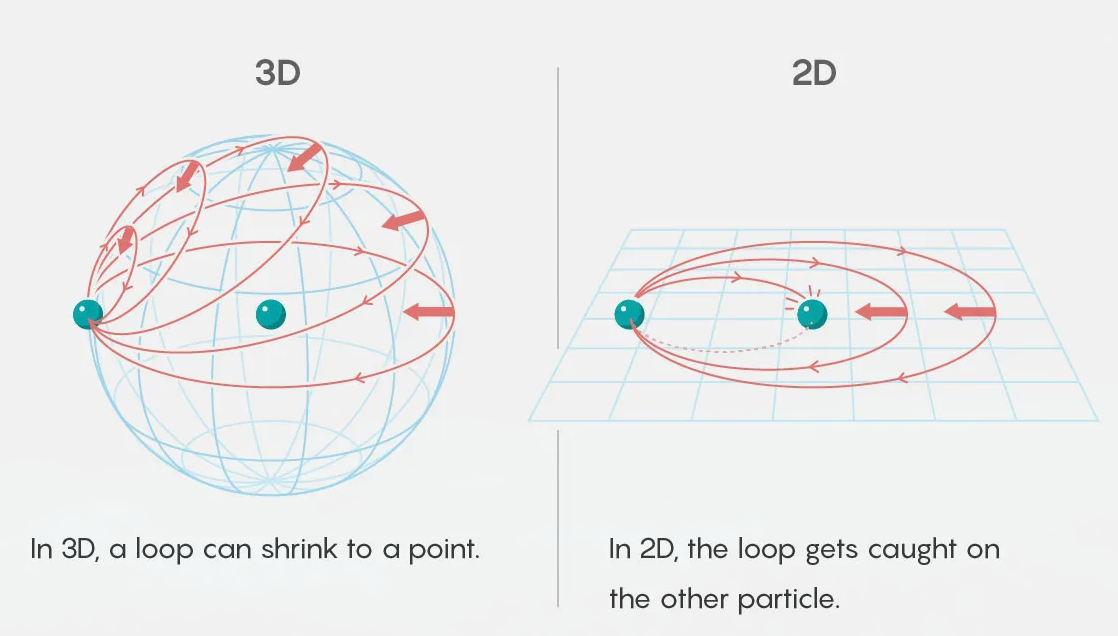
\includegraphics[width=0.8\textwidth]{figs/2d_v_3d_particle.png}
  \caption{Visualization of the difference between particle exchange in two and three dimensions. In three dimensions, the exchange loop can be shrunk to a point, making a double exchange topologically equivalent to leaving the particles unchanged. In two dimensions, the corresponding loop cannot be shrunk to a point without crossing the particle worldlines. This topological distinction allows anyons to exhibit non-trivial exchange statistics.{\color{red} $https://media.wired.com/photos/5ebf0488d58e99fafced8087/master/w_1600\%2Cc_limit/Science_Anyons-graphic-FINAL.jpg$}}
  \end{center}

  \label{fig:2d_v_3d_particle}
\end{figure}

A collection of non-Abelian anyons with fixed positions and fixed local quantum numbers can possess a non-trivial topological degeneracy. Quantum information can then be encoded in this degenerate subspace, while braiding the anyons implements unitary transformations within it. Since the resulting transformation depends only on the braid topology, and not on small local deformations of the path, this provides a possible route toward fault-tolerant quantum gates. In suitable schemes, braiding operations can be combined with additional ingredients to implement the gates needed for quantum computation.\\{\color{red}https://www.nature.com/articles/npjqi20151}\\ \\ 

One of the most promising candidates for realizing non-Abelian exchange statistics in condensed-matter systems is the Majorana zero mode (MZM), predicted to occur in certain topological superconductors. A Majorana zero mode is a zero-energy quasiparticle described by an operator that is equal to its own Hermitian conjugate. In one-dimensional topological superconductors, such modes can appear at the ends of the system. Unlike an ordinary fermionic mode, a single MZM can be viewed as ``half'' of a Dirac fermion: two Majorana operators can be combined to form one conventional fermionic operator,
\begin{equation}
    c = \frac{1}{2}(\gamma_1 + i\gamma_2)
\end{equation}
with the inverse relations
\begin{equation}
    \gamma_1 = c + c^\dagger, \qquad \gamma_2 = -i(c-c^\dagger).
\end{equation}
Here $\gamma_1$ and $\gamma_2$ are Majorana operators satisfying
\begin{equation}
    \gamma_i = \gamma_i^\dagger, \quad \{\gamma_i, \gamma_j\} = 2\delta_{ij}
\end{equation}
The non-Abelian character of MZMs is reflected in the fact that exchanging two of them produces a non-trivial unitary transformation on the degenerate ground-state manifold{\color{red}https://www.nature.com/articles/npjqi20151}.\\ 
The primary motivation for studying MZMs and their braiding properties is their combination of non-local encoding and spectral protection. When a fermionic state is formed from two spatially separated MZMs, local environmental noise cannot easily determine or flip the encoded state, because such an error would require coupling to both separated Majorana components. Therefore, local perturbations are strongly suppressed as a source of decoherence{\color{red}https://journals.aps.org/rmp/abstract/10.1103/RevModPhys.80.1083}.\\
MZMs also give rise to ground-state degeneracies. A system with $2n$ Majorana zero modes spans a $2^n$-dimensional fermionic Hilbert space associated with the occupations of $n$ non-local fermions. If the total fermion parity is fixed, the physical ground-state degeneracy is reduced to $2^{n-1}$. In either case, the useful low-energy manifold must be separated from excited states by a finite spectral gap, which protects the encoded information against thermal excitations.{\color{red}https://arxiv.org/abs/cond-mat/0010440}.\\
The remaining question is how such Majorana operators can emerge from an ordinary fermionic Hamiltonian. The Kitaev chain provides the minimal model where this mechanism can be seen explicitly, and it also gives the conceptual starting point for the Poor Man's Majorana systems studied in this thesis.





\subsection{Kitaev Chain and Poor Man's Majorana Systems}
Before discussing the Majorana models used in this thesis, we first introduce their theoretical origin: the Kitaev chain. The Kitaev chain, or Kitaev-Majorana chain, is a simplified model for a topological superconductor. First proposed by Alexei Kitaev in 2000 {\color{red}https://arxiv.org/pdf/cond-mat/0010440}, the Kitaev chain is a one-dimensional superconducting system that can host Majorana zero modes at its ends under certain conditions, illustrated in Figure~\ref{fig:kitaev}. The model is defined on a lattice of spinless fermions with nearest-neighbor hopping and superconducting pairing. 
The Hamiltonian of the Kitaev chain is
\begin{equation}
H = -\mu \sum_{j=1}^{N} \left(c_j^\dagger c_j - \frac{1}{2}\right)
- t \sum_{j=1}^{N-1} \left(c_j^\dagger c_{j+1} + c_{j+1}^\dagger c_j\right)
+ \Delta \sum_{j=1}^{N-1} \left(c_j c_{j+1} + c_{j+1}^\dagger c_j^\dagger\right),
\label{eq:kitaev_ham}
\end{equation}
Each term in Eq.~\ref{eq:kitaev_ham} has a clear physical interpretation. The first term represents the chemical potential $\mu$, which controls the filling of the fermionic states. The second term describes the hopping of fermions between neighboring sites with amplitude $t$. The third term represents $p$-wave superconducting pairing, where pairs of fermions are created or annihilated on adjacent sites with amplitude $\Delta$.\\
As shown schematically in Fig.~\ref{fig:kitaev}, the Kitaev chain has two distinct phases depending on the parameters $\mu$, $t$, and $\Delta$. In the trivial phase, the Majorana modes on the same site pair up to form conventional fermions, leaving no unpaired modes. In the topological phase, Majoranas on adjacent sites couple, leaving unpaired modes at the chain ends. These unpaired Majoranas combine into a non-local fermionic mode that can be occupied or empty without costing energy, leading to a twofold degeneracy in the ground state. This degeneracy is protected as long as local perturbations do not close the bulk gap or directly hybridize the edge modes.\\



\begin{figure}
  \centering
  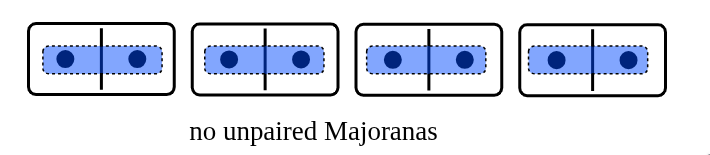
\includegraphics[width=0.45\textwidth]{figs/no_unpaired.png}
  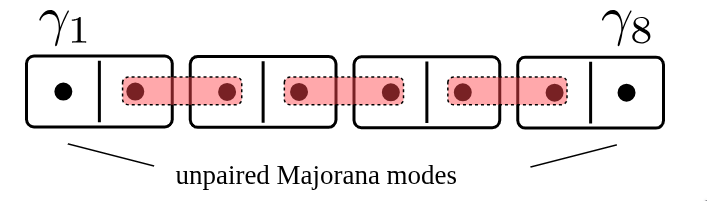
\includegraphics[width=0.45\textwidth]{figs/unpaired.png}
  \caption{Schematic representation of the Kitaev chain in its two distinct phases. Left: In the trivial phase, Majorana modes on the same site pair to form conventional fermions, leaving no unpaired modes. Right: In the topological phase, Majoranas on adjacent sites couple, leaving unpaired modes at the chain ends, which combine into a non-local fermionic mode. {\color{red}Topocondmat}}
  \label{fig:kitaev}
\end{figure}

The topological phase of the Kitaev chain is the basic model for the Majorana zero modes studied in this thesis. The goal is then to understand how similar Majorana-like physics can be engineered in more realistic systems.
\\ \\

\paragraph{Bulk Spectrum and Topological Phase\newline}

In order to determine when the Kitaev chain is topological, we need to consider the properties of the bulk spectrum. \\ 
For a translationally invariant chain, we can perform a Fourier transform to momentum space, which allows us to analyze the energy spectrum and identify the conditions for the topological phase. The Fourier transform is given by

\begin{equation}
  c_j = \frac{1}{\sqrt{N}} \sum_p e^{ipaj} c_p
\end{equation}
This transformation allows the Hamiltonian to be expressed in terms of momentum-space operators $c_p$ and $c_p^\dagger$. The resulting Hamiltonian in momentum space is
\begin{equation}
H = ∑_{ p}^{} ξ_p\left(c_p^{†} c_p - \frac{1}{2}\right) - ∑_{p}^{} t \cos p a + Δ ∑_{p}^{}\left(c_p^{†} c_{-p}^{†} e^{ipa} + c_{-p} c_p e^{-ipa}\right), 
\end{equation}

with $ξ_p = -μ - 2t \cos pa$ and $a$ being the lattice spacing. In the Bogoliubov--de Gennes formalism, the quasiparticle spectrum becomes
\begin{equation}
  E_{p,\pm} = \pm \sqrt{(\mu + 2t \cos{pa})^2 + 4\Delta^2 \sin^2{pa}}.
\end{equation}
Even though the Bogoliubov--de Gennes formalism describes a non-interacting quasiparticle problem, it still provides the basic topological picture that the interacting models in this thesis build on. In Fig.~\ref{fig:kitaev_bands}, we can see how the spectrum changes as the chemical potential $\mu$ is tuned. The presence of a gap is crucial for the stability of the Majorana modes, and the closing and reopening of this gap signals a topological phase transition.\\ \\
The quasiparticle spectrum is gapped for most parameter values, but the gap closes when
\[
|\mu| = 2|t|.
\]
This is also visible in Fig.~\ref{fig:kitaev_bands}. The gap closing marks the transition between the trivial and topological phases. When $\mu$ crosses this boundary, the ground state changes its topological character without requiring ordinary symmetry breaking {\color{red}Qtech}.\\
\begin{figure}
  \centering
    
    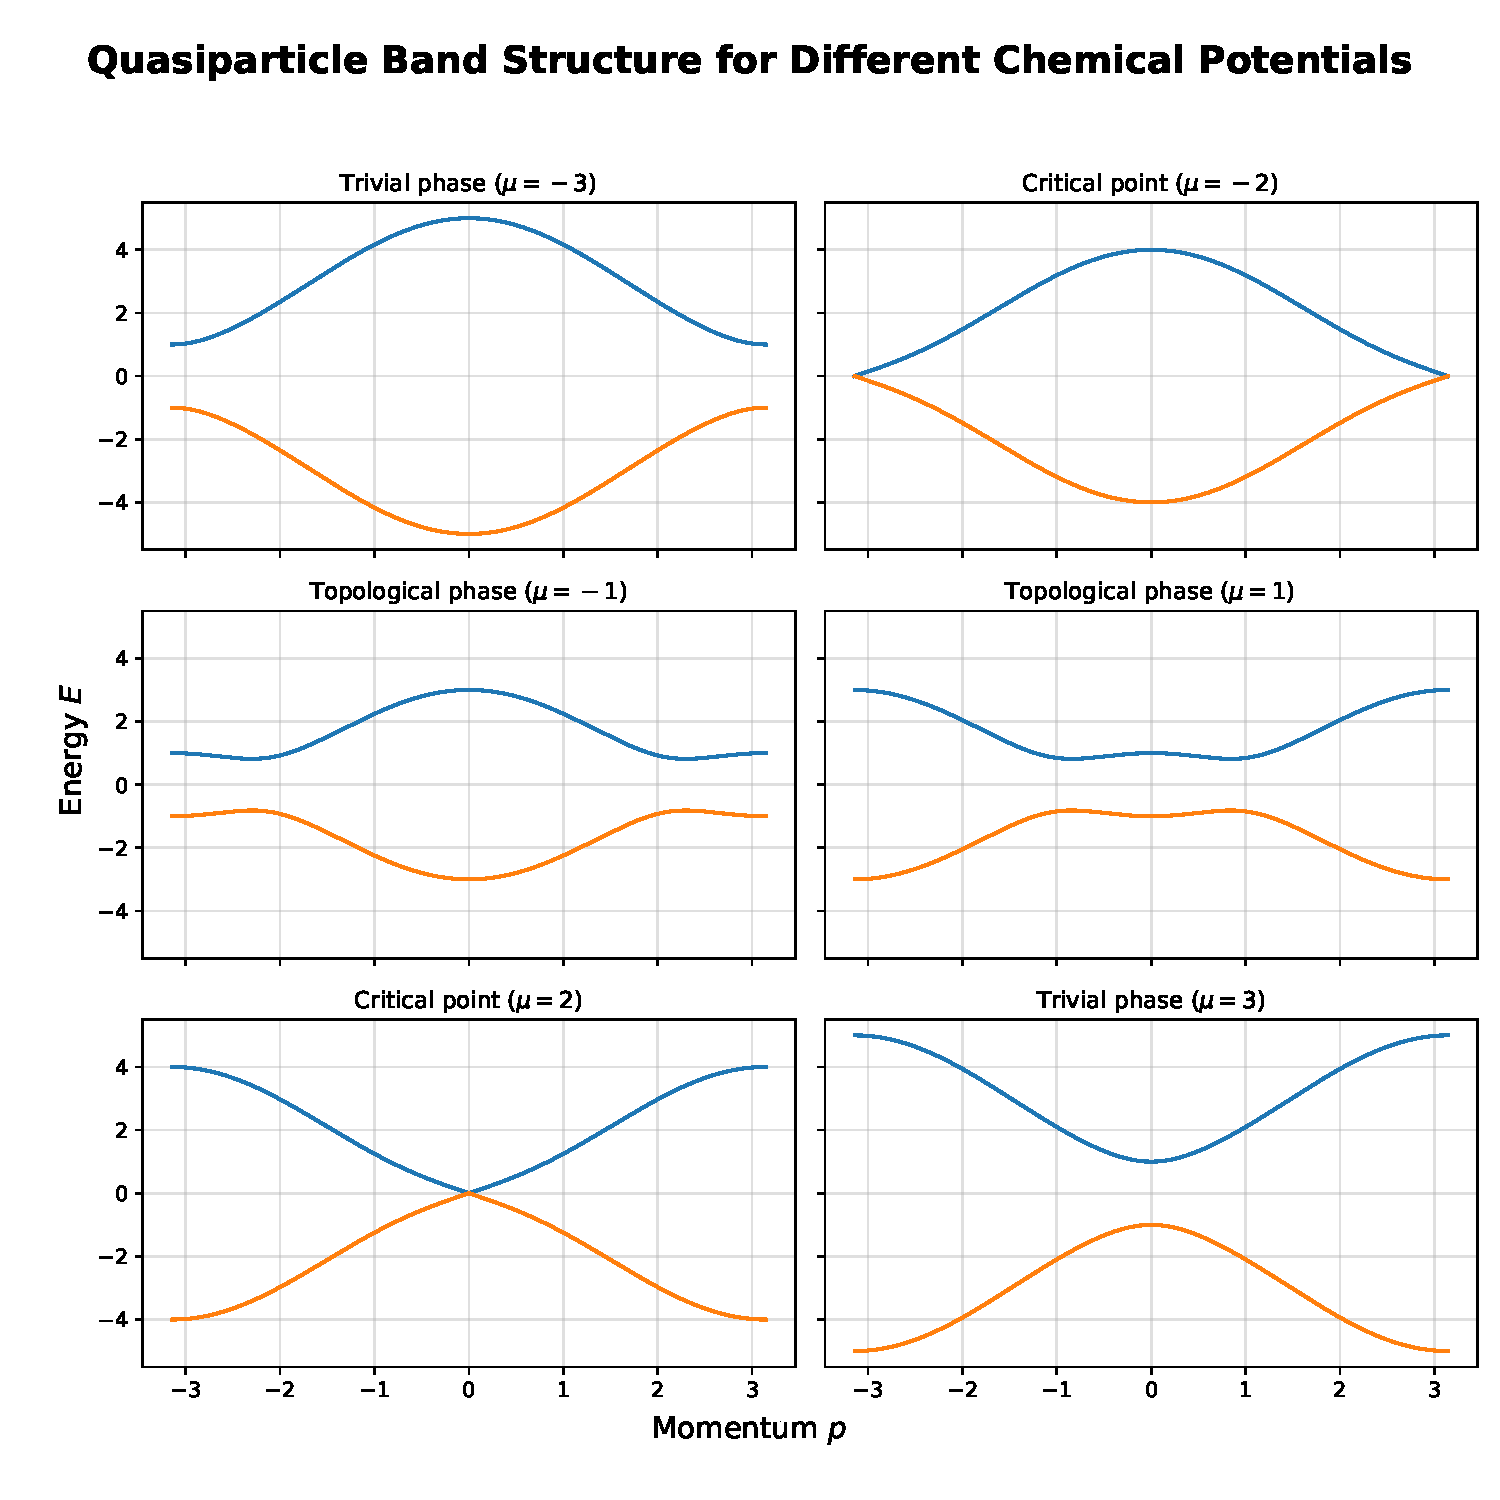
\includegraphics[width=.8\textwidth]{figs/band_structure.pdf}
    \caption{Quasiparticle energy spectrum of the Kitaev chain for different chemical potentials $\mu$. Left: In the trivial phase ($|\mu| > 2|t|$), the spectrum is fully gapped with no zero-energy modes. Right: In the topological phase ($|\mu| < 2|t|$), the gap closes and reopens, signaling the emergence of zero-energy edge modes.}
  \label{fig:kitaev_bands}
\end{figure}
\newpage

\paragraph{Majorana Representation and Zero Modes\newline}
Looking back at Fig.~\ref{fig:kitaev}, we want a representation that makes the unpaired edge modes more explicit. To do so, we express the fermionic operators in terms of Majorana operators. For each site $j$, we define two Majorana operators $\gamma_j^A$ and $\gamma_j^B$ as follows:
\begin{equation}
c_j = \frac{1}{2}(\gamma_j^A + i\gamma_j^B), \quad
c_j^\dagger = \frac{1}{2}(\gamma_j^A - i\gamma_j^B),
\label{eq:first_majorana_rep}
\end{equation}
where $\gamma_j^{A,B}$ satisfy $\{\gamma_j^\alpha, \gamma_k^\beta\} = 2\delta_{jk}\delta_{\alpha\beta}$ and $(\gamma_j^\alpha)^\dagger = \gamma_j^\alpha$. In the trivial phase, the Majorana operators pair on the same site. In the topological phase, and especially at the ideal point $t=\Delta$ and $\mu=0$, $\gamma_j^B$ couples to $\gamma_{j+1}^A$. This leaves two edge modes unpaired, $\gamma_1^A$ and $\gamma_N^B$, at the chain ends. These two unpaired Majoranas define a non-local fermionic mode,
\begin{equation}
  f = \frac{1}{2}(\gamma_1^A + i\gamma_N^B),
\end{equation}
which satisfies $\{f, f^\dagger\}=1$ and costs zero energy to occupy. This non-local fermionic mode creates the basis for the exploration of Majorana physics in this thesis, and it is the key to understanding how Majorana modes can be used for quantum computation. The occupation of this non-local mode corresponds to a twofold degeneracy in the ground state, which is protected as long as local perturbations do not close the bulk gap or directly hybridize the two edge modes. This non-local encoding of information is what gives Majorana modes their potential for fault-tolerant quantum computation, as local errors cannot easily access or change the encoded state.{\color{red}Qtech}


\paragraph{Poor Man's Majorana Systems\newline}

While the Kitaev chain is the minimal theoretical model, it assumes spinless fermions and intrinsic $p$-wave pairing. Real superconductors are usually spinful and dominated by conventional $s$-wave pairing. The Poor Man's Majorana (PMM) platform is a compact engineered system whose low-energy behavior can mimic a short Kitaev chain. The simplest version is a double quantum dot coupled through a superconducting segment. Each dot acts as a site, elastic cotunneling produces effective hopping, and crossed Andreev reflection produces an effective non-local pairing term.\\

The effective two-dot Hamiltonian can be written as
\begin{equation}
H = \sum_{i=L,R} \epsilon_i n_i
+ t (d_L^\dagger d_R + d_R^\dagger d_L)
+ \Delta (d_L^\dagger d_R^\dagger + d_R d_L)
+ U n_L n_R,
\label{eq:qdsqdh}
\end{equation}
where $d_{L/R}^\dagger$ and $d_{L/R}$ are creation and annihilation operators on the left and right dots, $n_i$ is the number operator, $\epsilon_{L,R}$ are the dot energy levels, $t$ is the elastic cotunneling amplitude, $\Delta$ is the crossed Andreev reflection amplitude, and $U$ is the interdot Coulomb interaction energy. The parameters map directly onto the Kitaev-chain language:
\begin{itemize}
    \item \textbf{Elastic cotunneling (ECT):} An electron tunnels coherently from one dot to the other through a virtual process in the superconductor. This produces the effective hopping amplitude $t$.
    \item \textbf{Crossed Andreev reflection (CAR):} A Cooper pair splits, with one electron entering each dot. This produces the non-local pairing amplitude $\Delta$.
    \item \textbf{On-site energy:} The dot energies $\epsilon_L$ and $\epsilon_R$ play the role of local chemical potentials.
\end{itemize}
At the ideal non-interacting sweet spot, $|\epsilon_L|=|\epsilon_R|=0$ and $|t|=|\Delta|$, the two-dot system develops Majorana-like states localized primarily on opposite dots. Since the system is finite and lacks a true bulk, these states are not topologically protected in the same sense as an infinite Kitaev chain. This is why they are referred to as Poor Man's Majoranas {\color{red}Qtech}.\\

For the purposes of this thesis, the PMM idea is generalized from two dots to interacting $n$-dot chains. A schematic representation is shown in Figure \ref{fig:PMM_setup}. Adding more dots introduces more tunable parameters and more possible low-energy structure, but it also makes the analytic sweet-spot problem much harder. This motivates the numerical optimization strategy discussed later in the thesis.
\begin{figure}
  \centering
  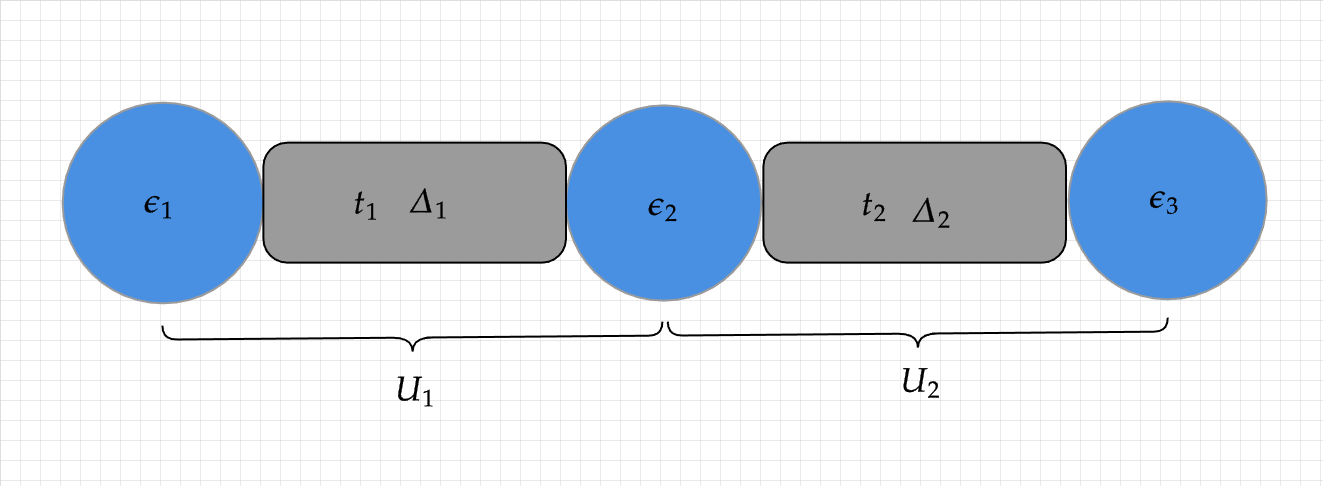
\includegraphics[width=0.8\textwidth]{figs/PMMSetup.png}
  \caption{Schematic representation of the PMM setup. The three quantum dots are represented by the blue circles, and the superconducting segments are represented by the grey rectangles. The tunable parameters of the system, such as the dot energy levels, ECT, CAR and the Coulomb interaction, are indicated by their respective labels. By tuning these parameters, we can access different regimes of the system and identify the sweet spots where Majorana-like modes emerge.}
  \label{fig:PMM_setup}
\end{figure}

\subsection{Diagnostics of Majorana-like States}
In a finite PMM system, the presence of low-energy states alone is not enough to claim Majorana physics. The states must also have the right parity structure, local indistinguishability, charge distribution, and Majorana-polarization profile. These diagnostics are especially important in interacting systems, where a low numerical energy splitting can appear for reasons that are not necessarily related to edge-localized Majorana modes.\\

\paragraph{Fermion Parity\newline}
The mean-field Hamiltonian of a superconductor does not conserve particle number, because particles can be added or removed in Cooper pairs. It does, however, conserve fermion parity. The parity operator can be written as
$$
P = (-1)^{N} = Π_n(1 - 2c_n ^{†} c_n),
$$
where $N$ is the total particle number. The eigenvalues of $P$ are $+1$ for even parity and $-1$ for odd parity. In a Majorana system, the two lowest states often differ by fermion parity, and near-degeneracy between these opposite-parity states is one of the central signatures of a Majorana-like mode {\color{red}Topocondmat}.\\

\paragraph{Energy Degeneracy and Spectral Gap \newline}
The first spectral signature is approximate degeneracy between even- and odd-parity states. In the ideal case, the ground states in the two parity sectors are exactly degenerate. In practice, a finite system will generally have a small splitting, and the goal is to make this splitting as small as possible compared with the excitation gap. The gap to higher excited states is also crucial: it protects the low-energy manifold from thermal excitations and helps justify projecting the dynamics onto a small subspace during braiding.{\color{red}Topocondmat}\\
\begin{figure}
  \centering
  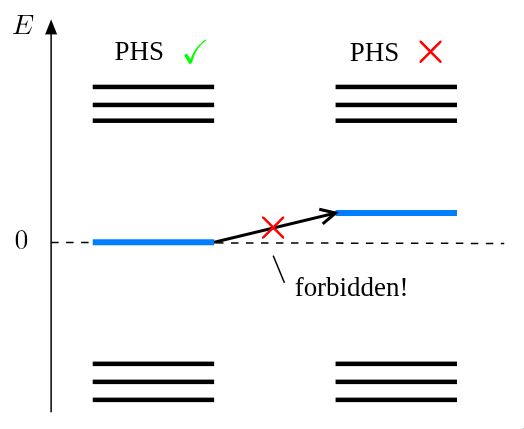
\includegraphics[width=0.5\textwidth]{figs/gs_symmetry}%
  \caption{Energy spectrum showing how the energy eigenvalues of the system must be symmetric around zero energy due to particle-hole symmetry \cite{Topocondmat}.}
  \label{fig:gs_symmetry}
\end{figure}

\paragraph{Local Distinguishability\newline}
A defining feature of spatially separated Majorana modes is that the encoded information is non-local. Local measurements should therefore not reveal whether the system is in the even or odd ground state. One way to quantify this is through the local distinguishability parameter
$$
\text{LD} = \frac{1}{N} \sum_{j=1}^{N} || \rho_j^o - \rho_j^e || = \frac{1}{N} \sum_{j=1}^{N} || \delta \rho_j ||.
$$
{\color{red}Lund1, VikMar}.
Here, $\rho_j^{o/e}$ are the reduced density matrices of site $j$ for the odd and even parity ground states, respectively, and $||\cdot||$ is the trace norm. A value close to zero indicates that the two states are locally indistinguishable, while a larger value indicates that local measurements can tell the two parity states apart.\\

\paragraph{Majorana Polarization\newline}
The Majorana polarization (MP) is used to quantify how closely the low-energy states resemble spatially localized Majorana modes. In an ideal PMM configuration, the polarization should be concentrated at the edge dots, with opposite signs on the two ends and little or no weight in the bulk. One useful definition is
$$
M_\alpha = \frac{W_\alpha^2 - Z_\alpha^2}{W_\alpha^2 + Z_\alpha^2},
$$
where
$$
W_\alpha = ∑_{\sigma} \bra{o} c_{\alpha\sigma} + c_{\alpha\sigma}^{†} \ket{e}, \quad Z_\alpha = i ∑_{\sigma} \bra{o} c_{\alpha\sigma} - c_{\alpha\sigma}^{†} \ket{e}.
$$
Here, $\alpha$ denotes the site index, $\sigma$ is the spin index, and $\ket{o}$ and $\ket{e}$ are the odd- and even-parity ground states. In an ideal sweet spot with two perfectly localized Majoranas, the edge values would satisfy $M_L=-M_R=\pm 1$ \cite{Qtech}.\\

\paragraph{Charge Expectation and Non-locality\newline}
Another diagnostic is the local charge expectation value in the even and odd states,
$$
\bra{e}n_{L(R)} \ket{e}, \quad \bra{o}n_{L(R)} \ket{o}.
$$
In the ideal case, these expectation values should be equal for the two parity states. A small charge difference means that the two states share the same local charge distribution, which is another way of saying that the parity information is stored non-locally rather than being visible on a single dot.\\

\paragraph{Optimization Motivation\newline}
For a simple two-dot system, the relevant tunable parameters are the dot energies, elastic cotunneling, crossed Andreev reflection, and interaction strength. For longer chains, the number of tunable parameters grows quickly. Since interactions and inhomogeneous parameters make it difficult to identify sweet spots analytically, the diagnostics above can be combined into a loss function and used to search numerically for promising Majorana-like regimes. The resulting loss landscape may contain many local minima, which motivates the repeated-restart and basin-hopping strategy described in the methods chapter.
\begin{figure}
\centering
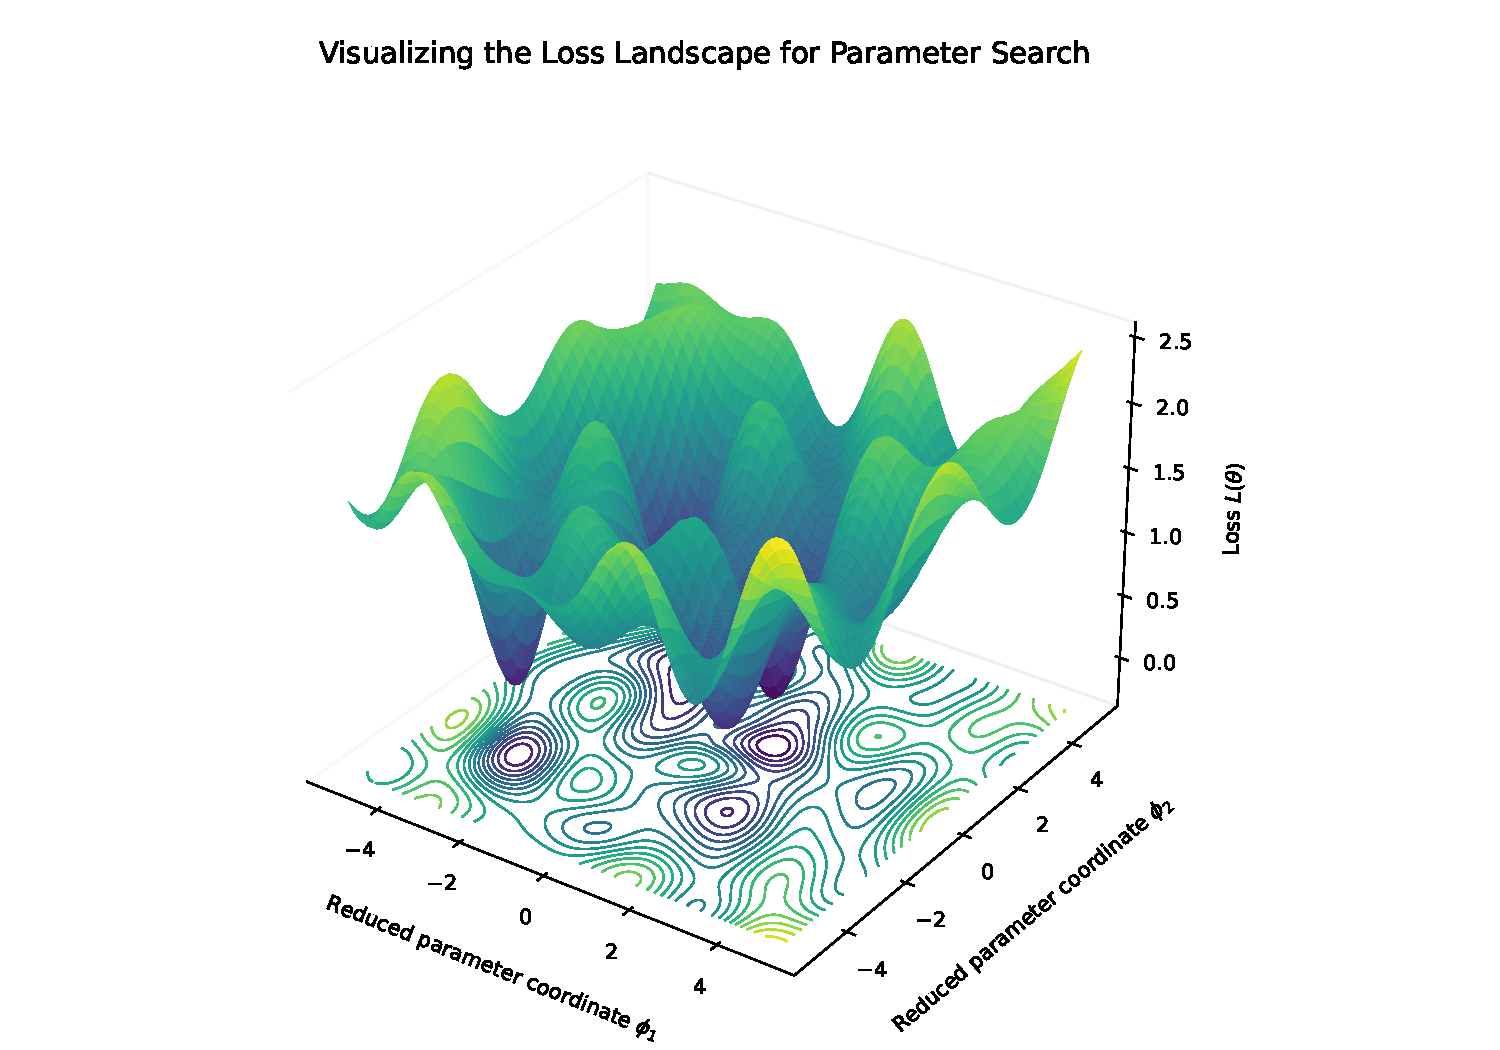
\includegraphics[width=\textwidth]{figs/3dparametersearch.pdf}
\caption{Visualization of the parameter space for an n-dot system, showing how multiple parameters and their combinations create a complex landscape with multiple local minima.}
\label{fig:paramVisualization}
\end{figure}

\subsection{Majorana Exchange and Braiding}
Braiding is the operation that makes Majorana modes useful for topological quantum computation. The basic idea is to exchange two Majorana modes adiabatically so that the quantum state transforms according to their non-Abelian statistics. Because the transformation is tied to the topology of the exchange, rather than to the exact microscopic path, braiding offers a route to gates that are less sensitive to local control errors. Braiding in the right patterns, with the right systems, can lead to the implementation of useful quantum gates.{\color{red} SOURCE}\\

\subsubsection{Quantum Gates}
In the circuit model of quantum computation, a gate is a unitary operation acting on one or more qubits. The Pauli gates are among the simplest examples:
\begin{equation}
X = \begin{pmatrix} 
0 & 1 \\
1 & 0
\end{pmatrix}, \quad
Y = \begin{pmatrix}
0 & -i \\
i & 0
\end{pmatrix}, \quad
Z = \begin{pmatrix}
1 & 0 \\
0 & -1
\end{pmatrix}.
\end{equation}
Acting on the basis states
\begin{equation}
\ket{0} = \begin{pmatrix}
1 \\
0
\end{pmatrix}, \quad
\ket{1} = \begin{pmatrix}
0 \\
1
\end{pmatrix},
\end{equation}
these gates produce
\begin{align*}
X\ket{0} &= \ket{1}, \quad X\ket{1} = \ket{0}, \\
Y\ket{0} &= i\ket{1}, \quad Y\ket{1} = -i\ket{0}, \\
Z\ket{0} &= \ket{0}, \quad Z\ket{1} = -\ket{1}.
\end{align*}
\begin{figure}
  \centering
  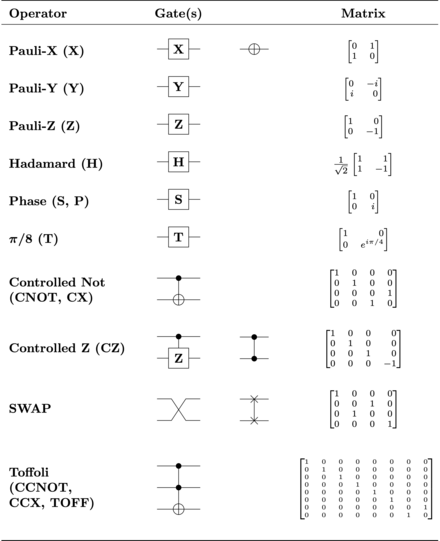
\includegraphics[width = 0.5\textwidth]{figs/Quantum_logic_gates.png}
  \label{fig:quantum_gates}
    \caption{List of common quantum gates and their matrix representations. {\color{red} Wikipedia Quantum logic gates}}
\end{figure}

\paragraph{Pauli Gates in Fermionic Language}
To connect gates to Majorana systems, it is useful to express simple qubit operations in terms of fermionic operators. For a two-site system with fermionic operators $c_1$ and $c_2$, one can write
\begin{align*}
  X &= c_1 ^{†} c_2 + c_2 ^{†} c_1, \\
  Y &= -i(c_1 ^{†} c_2 - c_2 ^{†} c_1), \\
  Z &= c_1 ^{†} c_1 - c_2 ^{†} c_2.
\end{align*}
These expressions show how qubit operations can be represented through hopping-like and occupation-like operators in a fermionic system.\\

\subsubsection{Jordan-Wigner Transformation}
The Jordan-Wigner transformation maps spin operators to fermionic creation and annihilation operators. Starting from
\begin{align*}
\sigma_j^+ &= \frac{1}{2}(\sigma_j^x + i\sigma_j^y) \equiv f_j ^{†}, \\
\sigma_j^- &= \frac{1}{2}(\sigma_j^x - i\sigma_j^y) \equiv f_j, \\
\sigma_j^z &= 2f_j ^{†} f_j - 1,
\end{align*}
the same-site fermionic relation is correct, but operators on different sites commute instead of anticommute. To fix this, one introduces a string of $\sigma^z$ operators,
\begin{equation}
  a_j^{†} = Π_{k=1}^{j-1} (-\sigma_k^z) \cdot f_j^{†}, \quad a_j = Π_{k=1}^{j-1} (-\sigma_k^z) \cdot f_j,
\end{equation}
which gives
\begin{align*}
\{a_j^{†}, a_k\} &= \delta_{jk}, \\
\{a_j^{†}, a_k^{†}\} &= 0, \\
\{a_j, a_k\} &= 0.
\end{align*}
{\color{red} SOURCE JW WIKIPEDIA}\\

\paragraph{Pauli Matrices in the Majorana Representation}
Using the Majorana representation from Eq.~\ref{eq:first_majorana_rep}, define four Majorana operators by
\begin{align*}
  c_1 &= (\gamma_0 + i \gamma_1)/2, \quad c_1 ^{†} = (\gamma_0 - i \gamma_1)/2, \\
  c_2 &= (\gamma_2 + i \gamma_3)/2, \quad c_2 ^{†} = (\gamma_2 - i \gamma_3)/2.
\end{align*}
The Pauli operators can then be expressed as Majorana bilinears. In a fixed parity subspace, these simplify to
\begin{align*}
  X &= \frac{i}{2} (\gamma_0\gamma_3 - \gamma_1\gamma_2) = i\gamma_0\gamma_3 = -i\gamma_1\gamma_2, \\
  Y &= -\frac{i}{2} (\gamma_0\gamma_2 + \gamma_1\gamma_3) = -i \gamma_0\gamma_2 = -i \gamma_1\gamma_3, \\
  Z &= \frac{i}{2} (\gamma_0\gamma_1 + \gamma_2\gamma_3) = i\gamma_0\gamma_1 = i\gamma_2\gamma_3.
\end{align*}
This is the key connection between qubit gates and Majorana couplings: turning on controlled bilinear couplings between Majoranas implements rotations in the encoded qubit space.\\

\paragraph{Majorana Exchange Gates}
The unitary operator associated with exchanging two Majoranas $\gamma_i$ and $\gamma_j$ should satisfy
\begin{align*}
B_{ij} \gamma_i B_{ij} ^{†} &= \gamma_j, \\
B_{ij} \gamma_j B_{ij} ^{†} &= -\gamma_i, \\
B_{ij} \gamma_k B_{ij} ^{†} &= \gamma_k \quad \text{for } k \neq i,j.
\end{align*}
The corresponding exchange operator can be written as
\begin{equation}
B_{ij} = \frac{i}{\sqrt{2}} (1 - \gamma_i \gamma_j), \quad B_{ij} ^{†} = \frac{1-i}{\sqrt{2}} (1 + \gamma_i \gamma_j).
\end{equation}
Squaring exchange operations gives transformations directly related to Pauli gates:
\begin{align*}
B_{12}^2 &= -i\gamma_1\gamma_2 = -X, \\
B_{03}^2 &= i\gamma_0\gamma_3 = X, \\
B_{02}^2 &= i\gamma_0\gamma_2 = -Y,\\
B_{13}^2 &= i\gamma_1\gamma_3 = -Y,\\
B_{01}^2 &= i\gamma_0\gamma_1 =  Z,\\
B_{23}^2 &= i\gamma_2\gamma_3 =  -Z.
\end{align*}

\subsection{Projected Subspaces, Kato Transport and Braid Unitaries}
\subsubsection{Kato Berry Phase}
The Berry phase is a geometric phase acquired by a quantum state during adiabatic evolution around a closed loop in parameter space. For a non-degenerate eigenstate, the state returns to itself up to a phase. This phase has a dynamical part, which depends on the time scale and the energy of the state, and a geometric part, which depends only on the path in parameter space. The geometric contribution is the Berry phase.\\

For a degenerate subspace, the situation is richer. The adiabatic evolution can mix states within the degenerate manifold, so the Berry phase becomes a matrix rather than a scalar phase. In this thesis, this non-Abelian Berry matrix is what determines the braid unitary acting on the Majorana qubit space.\\

The Kato formulation provides a convenient way to compute this adiabatic transport. Instead of tracking individual eigenvectors and their phases, one works directly with the projector $P(t)$ onto the relevant low-energy subspace. The Kato evolution satisfies
$$
\partial_{t}U_t = i \left[P, \partial_{t}P\right]U_t, \qquad
U_0 = I.
$$
The final unitary $U_T$ is the non-Abelian Berry phase associated with the path. In numerical calculations, $P(t)$ is obtained by diagonalizing the Hamiltonian at each time step and constructing the projector onto the chosen low-energy manifold.\\

\subsubsection{Effective Braiding Hamiltonian}
As a reference model, assume that the system contains four Majorana modes $\gamma_0$, $\gamma_1$, $\gamma_2$, and $\gamma_3$ involved in the braid. A useful physical picture is a Y-junction made from three PMM subsystems, where one central Majorana is coupled sequentially to different neighboring Majoranas.\\
\begin{figure}
  \centering
  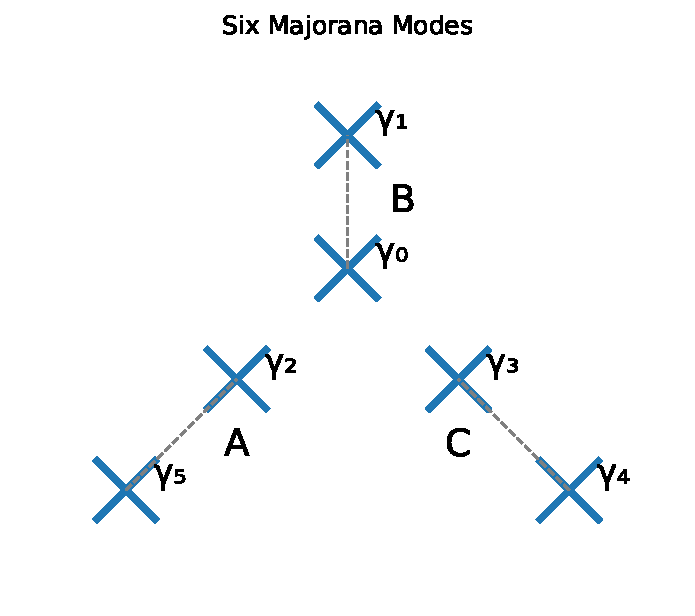
\includegraphics[width=0.5\textwidth]{figs/sixmajoranas.pdf}
  \caption{Schematic representation of a system hosting six majoranas. The illustrations shows pairs of two and two Majoranas coupling together, in a Y-junction, each pair form a subsystem that can be described by a Poor Man’s Majorana setup, A, B and C.}
  \label{fig:6_majoranas}
\end{figure}
In Fig.~\ref{fig:6_majoranas}, the four Majoranas $\gamma_0$, $\gamma_1$, $\gamma_2$, and $\gamma_3$ are the modes actively used in the braid, while $\gamma_4$ and $\gamma_5$ form a spectator pair. The ideal effective Hamiltonian can be written as
\begin{equation}
  \begin{aligned}
    H = &\Delta_{01} i\gamma_0\gamma_1 + \\
    &\Delta_{02} i\gamma_0\gamma_2 + \\
    &\Delta_{03} i\gamma_0\gamma_3,
  \end{aligned}
  \label{eq:H_eff}
\end{equation}
where $\Delta_{ij}$ is a tunable coupling between Majoranas $\gamma_i$ and $\gamma_j$. By turning these couplings on and off in a controlled sequence, the system can implement an effective exchange operation.\\

In a microscopic PMM device, the tunable quantities are not abstract Majorana bilinears, but physical hopping and pairing couplings between dots or subsystems. A junction between two PMM subsystems can be modeled by
\begin{equation}
  H_{JuncAB} = t_{AB} (d_{A} ^{†} d_{B} + d_{B} ^{†} d_{A}) + \Delta_{AB} (d_{A} ^{†} d_{B} ^{†} + d_{B} d_{A}),
  \label{eq:junctionHamiltonian}
\end{equation}
which is the same type of elastic cotunneling and crossed-Andreev pairing structure appearing in the PMM Hamiltonian. This motivates comparing two related braid constructions: one built from ideal or energy-level Majorana operators, and one built from projected microscopic local operators.\\

\subsubsection{Energy-Level and Local-Operator Braids}
The energy-level construction starts from the parity-resolved eigenstates of each optimized subsystem. Even and odd states are paired by energy, and effective Majorana operators are formed from combinations such as
$$
\gamma_1 \sim \ket{o}\bra{e} + \ket{e}\bra{o}, \qquad
\gamma_2 \sim i(\ket{o}\bra{e} - \ket{e}\bra{o}).
$$
This construction asks whether the spectrum itself supports a clean Majorana-like exchange channel.\\

The local-operator construction instead begins with microscopic endpoint operators, such as local combinations of $c^\dagger$ and $c$, and projects them into the retained low-energy subspace. This construction asks whether the same exchange channel is actually accessed by physical local couplings in the device. The distinction between these two constructions is important in this thesis, because the optimized spectrum can support an effective Majorana algebra even when the projected local operators only approximate the ideal energy-level Majoranas.

% \newpage
\chapter{Method}

This chapter describes the methods used to optimize the Majorana modes in the junction setup and to analyze their properties. We first discuss the parameter optimization process, including the model parameterization, loss function design based on Majorana criteria, and the optimization strategy. Next, we detail the post-optimization analysis of the setup, covering Hamiltonian reconstruction, parity classification, and various diagnostics. Finally, we describe the braiding protocol implemented in an effective Majorana model and how we validate the results using gate-validation checks.

\section{Numerical PMM Hamiltonian and Basis}
The numerical calculations are built from the spinless $n$-dot PMM Hamiltonian introduced in the theory chapter. This section specifies how that model is represented in the code: which Hamiltonian is diagonalized, which basis is used, how the fermionic operators are constructed, and how the model parameters are organized before optimization and braiding calculations.

\subsection{Single-Chain Hamiltonian}
For a single $n$-dot PMM chain, the Hamiltonian used in the optimization and diagnostic calculations is
\begin{equation}
H_{\mathrm{PMM}}
=
\sum_{i=1}^{n} \epsilon_i n_i
+ \sum_{i=1}^{n-1}
\left[
-t_i\left(c_i^\dagger c_{i+1}+c_{i+1}^\dagger c_i\right)
+\Delta_i\left(c_i c_{i+1}+c_{i+1}^\dagger c_i^\dagger\right)
+U_i n_i n_{i+1}
\right].
\label{eq:method_pmm_hamiltonian}
\end{equation}
Here $c_i^\dagger$ and $c_i$ create and annihilate a spinless fermion on dot $i$, and $n_i=c_i^\dagger c_i$ is the corresponding number operator. The onsite energies $\epsilon_i$ play the role of local chemical potentials, $t_i$ are elastic cotunneling amplitudes, $\Delta_i$ are crossed-Andreev pairing amplitudes, and $U_i$ are nearest-neighbor density-density interaction strengths.

\subsection{Many-Body Fock Basis}
All operators are represented in the full many-body Fock basis. For a chain with $n$ dots, a basis state is specified by the occupation pattern
\begin{equation}
\ket{n_1 n_2 \cdots n_n},
\qquad
n_i\in\{0,1\},
\end{equation}
so the Hilbert-space dimension of a single chain is $2^n$. Diagonalizing Eq.~\ref{eq:method_pmm_hamiltonian} in this basis gives the full many-body spectrum and eigenstates used to calculate the Majorana diagnostics.

For braiding calculations, several optimized chains are combined into a larger Hilbert space. If $D$ identical PMM subsystems are used, each containing $n$ dots, the total number of fermionic sites is $N_{\mathrm{tot}}=Dn$ and the full Hilbert-space dimension is $2^{N_{\mathrm{tot}}}$. In the three-arm braiding geometry used later, $D=3$, corresponding to subsystems $A$, $B$, and $C$.

\subsection{Jordan-Wigner Construction of Fermionic Operators}
\label{sec:method-jordan-wigner-construction}
Using the Jordan-Wigner construction introduced in Sec.~\ref{sec:theory-jordan-wigner}, the code builds fermionic creation and annihilation operators from local spin raising and lowering operators. For site $j$, the operators are represented schematically as
\begin{equation}
c_j^\dagger =
\left[\prod_{k<j}(-\sigma_k^z)\right]\sigma_j^+,
\qquad
c_j =
\left[\prod_{k<j}(-\sigma_k^z)\right]\sigma_j^-.
\label{eq:method_jw_operators}
\end{equation}
The same construction is used for single-chain calculations and for the enlarged three-subsystem Hilbert space.

Once the creation and annihilation operators have been constructed, the code precomputes the basic operator products needed repeatedly:
\begin{equation}
n_i=c_i^\dagger c_i,\qquad
h_{ij}=c_i^\dagger c_j+c_j^\dagger c_i,\qquad
p_{ij}=c_i^\dagger c_j^\dagger+c_j c_i,\qquad
d_{ij}=n_i n_j .
\end{equation}
These building blocks are then combined with the parameter values in Eq.~\ref{eq:method_pmm_hamiltonian} to assemble the Hamiltonian matrix. 
For the three-subsystem geometry, the Jordan-Wigner ordering is
$$
A_1, A_2, \ldots, A_n, B_1, B_2, \ldots, B_n, C_1, C_2, \ldots, C_n.
$$
Operators acting on subsystem B therefore carry a Jordan-Wigner string over all sites in subsystem A, while all operators acting on subsystem C carry a string over all sites in both A and B.

The parameter conventions used when assembling this Hamiltonian during optimization are described in Sec.~\ref{sec:method-optimization-vector}.

\section{Parameter Optimization and Loss Function}
The purpose of the optimization is to find parameter regimes where the finite PMM chain has the spectral and local signatures of Majorana-like states. The theory chapter defined the physical criteria; here they are turned into a numerical objective. For each trial parameter vector, the Hamiltonian in Eq.~\ref{eq:method_pmm_hamiltonian} is constructed, diagonalized, separated into parity sectors, and assigned a scalar loss. The optimizer then updates only the free parameters, while fixed parameters are reinserted when the physical Hamiltonian is rebuilt.

\subsection{Optimization Vector and Parameter Reconstruction}
\label{sec:method-optimization-vector}
The Hamiltonian in Eq.~\ref{eq:method_pmm_hamiltonian} is specified by the physical parameters $\{t_i,U_i,\epsilon_i,\Delta_i\}$. In the numerical implementation, each group of parameters can be fixed, homogeneous, or inhomogeneous. A fixed parameter is held at a prescribed value and is not included in the optimization vector. A homogeneous parameter has the same value on every site or bond, while an inhomogeneous parameter is allowed to vary independently from site to site or bond to bond. This makes it possible to compare restricted ansatz with more flexible parameter searches using the same Hamiltonian-building routine.

The optimizer therefore does not act directly on a full dictionary of physical parameters. Instead, it acts on a reduced real vector $\theta$ containing only the entries that are free in the chosen parameter configuration. For example, if $t_i$ is fixed and $U_i$ is fixed to a selected interaction strength, then those entries are excluded from $\theta$. If a parameter is homogeneous, only one number is included, or if it is inhomogeneous, one number is included for each site or bond.

The reduced vector is converted back into a parameter dictionary before the Hamiltonian is evaluated. Schematically,
\begin{equation}
\theta
\longrightarrow
\{t_i,U_i,\epsilon_i,\Delta_i\}
\longrightarrow
H_{\mathrm{PMM}}(\theta).
\end{equation}
During this conversion, fixed values are reinserted, homogeneous values are expanded across all sites or bonds when needed, and positive couplings such as $t_i$, $U_i$, and $\Delta_i$ are constrained to be non-negative. This separation lets the optimizer work with a compact vector while the Hamiltonian is still assembled from physical parameters.

In the optimization runs, the hopping amplitudes are fixed to $t_i=1$, while the interaction strength $U$ is fixed to the value being studied. The remaining parameters, the onsite energies $\epsilon_i$ and pairing amplitudes $\Delta_i$, are optimized. Fixing the hopping scale prevents the optimizer from lowering the loss through a trivial global rescaling of the kinetic energy, and instead forces the search to find nontrivial onsite and pairing profiles for each interaction strength. This also rules out the possibility of blowing up all other parameters in order to suppress the relative effect of interactions, which would be an unphysical way to achieve a low loss in the strongly interacting regime.

For each system size $n$ and interaction strength $U$, the lowest-loss physical parameter set is stored and later reused in the diagnostic and braiding calculations. The same parameter convention is also used when constructing the three-subsystem braiding geometry, as the optimized single-chain parameters define each subsystem, while additional inter-subsystem couplings are introduced only in the braiding-model sections below.

\subsection{Parity-Resolved Spectral Loss}
For each trial Hamiltonian, the full many-body spectrum is obtained by exact diagonalization. The eigenstates are then classified by the total fermion parity operator,
\begin{equation}
P_{\mathrm{tot}}=\prod_{i=1}^{n}(1-2n_i).
\end{equation}
This gives two ordered energy lists, one in the even sector and one in the odd sector,
\begin{equation}
\{E_k^{(e)}\},
\qquad
\{E_k^{(o)}\}.
\end{equation}
The loss function compares these parity partners level by level. For the parity-conserving Hamiltonians considered here, the even and odd sectors have equal dimension. The implementation nevertheless checks this explicitly, so that numerical or construction errors in the parity classification do not enter the loss evaluation.

The first loss contribution penalizes the energy splitting between even- and odd-parity partners,
\begin{equation}
\delta_k = \left|E_k^{(e)}-E_k^{(o)}\right|.
\end{equation}
As discussed in Sec.~\ref{sec:theory-parity-resolved-spectrum}, small even--odd splittings are one of the main spectral signatures of Majorana-like states. In the loss, these splittings are weighted more strongly at low energy. If $N_p$ parity pairs are used, the implementation defines a decreasing weight array
\begin{equation}
w_{\ell}
=
\left[
w_{\mathrm{max}}
-
\frac{\ell}{2N_p-2}
\left(
w_{\mathrm{max}}-w_{\mathrm{min}}
\right)
\right]^2,
\qquad
\ell=0,\ldots,2N_p-2,
\end{equation}
with $w_{\mathrm{max}}=3$ and $w_{\mathrm{min}}=0.1$. The degeneracy contribution is
\begin{equation}
\mathcal{L}_{\mathrm{deg}}
=
\sum_{k=0}^{N_p-1} w_k \left|E_k^{(e)}-E_k^{(o)}\right|.
\end{equation}
This term encourages the optimizer to produce an approximately parity-paired spectrum, with particular emphasis on the lowest-energy states.

The first $N_p$ entries of the weight array are used for the degeneracy term, while the remaining $N_p-1$ entries are used for the excitation-gap term. For adjacent parity pairs, the relevant gap is taken as
\begin{equation}
\Delta_k
=
\min\left(
E_{k+1}^{(e)}-E_k^{(e)},
E_{k+1}^{(o)}-E_k^{(o)}
\right).
\end{equation}
This $\Delta_k$ is the smaller spacing between adjacent levels in the two parity sectors. The corresponding weight is $w_{N_p+k}$.

Small gaps are penalized using a smooth threshold function,
\begin{equation}
\mathcal{L}_{\mathrm{gap}}
=
\sum_{k=0}^{N_p-2} w_{N_p+k}\,
\mathrm{softplus}
\left(
\Delta_{\mathrm{target}}-\Delta_k
\right),
\end{equation}
where $\Delta_{\mathrm{target}}$ is the desired minimum gap scale, and the softplus function is defined as $\mathrm{softplus}(x) = \log(1 + e^x)$\cite{NIPS2000_44968aec}.


\subsection{Charge and Majorana-Polarization Terms}
The local part of the loss turns the charge and Majorana-polarization diagnostics from Secs.~\ref{sec:theory-local-distinguishability} and \ref{sec:theory-majorana-polarization} into numerical penalties. The charge penalty measures how differently the even and odd partners occupy each site,
\begin{equation}
\mathcal{L}_{Q}
=
\sum_{k}\sum_{j}
\left|
\bra{e_k}n_j\ket{e_k}
-
\bra{o_k}n_j\ket{o_k}
\right|.
\end{equation}
This is the implementation form of the site-resolved charge-difference diagnostic.

The Majorana-polarization diagnostic itself was defined in Sec.~\ref{sec:theory-majorana-polarization}. In the optimizer, the corresponding penalty is implemented directly from the parity-changing matrix elements of the two local Majorana components $\gamma_{j,1}=c_j^\dagger+c_j$ and $\gamma_{j,2}=i(c_j^\dagger-c_j)$. For parity pair $k$ and site $j$, the code forms
\begin{equation}
\widetilde{M}_{k,j}
=
\left(
\bra{o_k}\gamma_{j,1}\ket{e_k}
\right)^2
+
\left(
\bra{o_k}\gamma_{j,2}\ket{e_k}
\right)^2 .
\end{equation}
The target profile is concentrated on the two ends of the chain with opposite sign,
\begin{equation}
\widetilde{M}^{\mathrm{tar}}_{k,1}=1,
\qquad
\widetilde{M}^{\mathrm{tar}}_{k,n}=-1,
\qquad
\widetilde{M}^{\mathrm{tar}}_{k,j}=0
\quad
(1<j<n).
\end{equation}
The sign of this target pattern is allowed to flip, since exchanging the labels of the two Majorana components changes the overall sign but not the physical localization pattern. The implemented Majorana-polarization penalty is therefore
\begin{equation}
\mathcal{L}_{\mathrm{MP}}
=
\min_{\sigma=\pm1}
\left|
\sum_{k,j}
\left(
\widetilde{M}_{k,j}
-
\sigma \widetilde{M}^{\mathrm{tar}}_{k,j}
\right)^2
\right|.
\end{equation}

\subsection{Total Normalized Loss}
The full loss is a sum of the spectral and local contributions. The implemented total loss is
\begin{equation}
\mathcal{L}
=
\frac{
\mathcal{L}_{\mathrm{deg}}
+
\mathcal{L}_{\mathrm{gap}}
+
\mathcal{L}_{Q}
+
\mathcal{L}_{\mathrm{MP}}
}{
\overline{|E|}+\eta
},
\end{equation}
where $\overline{|E|}$ is the mean absolute energy scale of the spectrum and $\eta$ is a small numerical offset. The spectral weights are already included in $\mathcal{L}_{\mathrm{deg}}$ and $\mathcal{L}_{\mathrm{gap}}$.

The normalization by $\overline{|E|}$ makes the spectral part of the loss less sensitive to the overall energy scale of a trial Hamiltonian. However, this normalization is not invariant under a uniform energy shift $H\mapsto H+\alpha\mathbb{1}$, since such a shift changes the absolute energies but leaves gaps and eigenvectors unchanged. In the parametrization used here there is no independent identity-shift parameter, so the optimizer does not explore such shifts directly.

A further limitation is that the same denominator also rescales the charge and Majorana-polarization penalties. These terms are dimensionless eigenvector diagnostics rather than energy penalties, so dividing them by an energy scale can make their contribution smaller when the spectrum becomes larger, even if the local Majorana quality does not improve. This possible bias is partly mitigated by fixing the hopping scale to $t=1$ and fixing $U$ during each optimization run, but the scalar loss should still be interpreted together with the separate spectral and local diagnostics.



\subsection{Search Strategy}
The resulting loss landscape is non-convex, especially once interactions are included. The numerical search therefore combines local gradient-based optimization with a basin-hopping procedure. The local optimizer is Adam, implemented with PyTorch automatic differentiation \cite{paszke2017automatic,kingma2014adam}.

At each Adam step, the reduced vector $\theta$ is converted into physical parameters, the Hamiltonian is constructed and diagonalized, and PyTorch automatic differentiation computes the gradient of the loss with respect to $\theta$.

The Adam update can be written as
\begin{equation}
\theta_k
=
\theta_{k-1}
-
\eta_{\mathrm{Adam}}
\frac{\hat{m}_k}{\sqrt{\hat{v}_k}+\varepsilon_{\mathrm{Adam}}},
\end{equation}
where $\eta_{\mathrm{Adam}}$ is the learning rate, and $\hat{m}_k$ and $\hat{v}_k$ are the bias-corrected moving averages of the gradient and squared gradient, respectively \cite{kingma2014adam}. In the implementation, Adam is called with learning rate $\eta_{\mathrm{Adam}}=0.05$, while the remaining Adam parameters are left at the PyTorch defaults, $\beta_1=0.9$, $\beta_2=0.999$, and $\varepsilon_{\mathrm{Adam}}=10^{-8}$. The parameters $\beta_1$ and $\beta_2$ set the moving averages that enter $\hat{m}_k$ and $\hat{v}_k$.

The numerical implementation of the Adam and basin-hopping search starts from a current parameter vector $\theta_{\mathrm{current}}$. A basin-hop is generated by drawing a trial vector
\begin{equation}
\theta_{\mathrm{trial}}
=
\theta_{\mathrm{current}}+0.25\,\xi,
\end{equation}
where the components of $\xi$ are normally distributed with zero mean and unit variance. Around this trial vector, we perform $6$ restarted Adam runs, each with an additional random perturbation,
\begin{equation}
\theta_{\mathrm{trial}}+\delta^{(r)},
\qquad
\delta_i^{(r)}\sim \mathrm{Unif}(-0.8,0.8).
\end{equation}
The scale $0.8$ was kept fixed as a practical perturbation scale, so that each basin-hop proposal is tested by several local Adam searches rather than a single trajectory. Each restarted run uses $300$ Adam iterations. The lowest-loss result from these restarts is used as the candidate for that basin-hopping step.

If the candidate has lower loss than the current vector, it is accepted. A candidate with higher loss is accepted with probability
\begin{equation}
p
=
\exp\left[
-\left(
\mathcal{L}_{\mathrm{cand}}-\mathcal{L}_{\mathrm{current}}
\right)
\right].
\end{equation}
This allows the search to occasionally leave a local basin instead of always moving downhill. The full basin-hopping search uses $30$ such steps for each pair $(n,U)$.

These search hyperparameters were not optimized systematically. They were kept fixed as practical settings chosen to balance exploration of the loss landscape against computational cost. For each pair $(n,U)$, the best configuration found by this procedure is stored together with its loss, parameter configuration, and reconstructed physical parameters.


\section{Post-Optimization Diagnostics}
The optimization procedure returns candidate parameter sets ranked by a scalar loss. Since this loss combines several criteria, a low value does not by itself show which Majorana signatures are actually present. For each pair $(n,U)$, the lowest-loss parameter set is therefore used to rebuild and diagonalize $H_{\mathrm{PMM}}(\theta_{\mathrm{opt}})$, after which the parity, charge, and Majorana-polarization diagnostics introduced in the theory chapter and used in the loss function above are evaluated separately.

For plotting and comparison, the parity-resolved spectrum is shifted so that the lowest state in either parity sector has energy zero. The reported spectral quantities are the splitting of the lowest even--odd pair,
\begin{equation}
\delta_0 =
\left|
E_0^{(e)}-E_0^{(o)}
\right|.
\label{eq:method_ground_state_splitting}
\end{equation}
The corresponding gap from this lowest pair to the nearest excited state is
\begin{equation}
\Delta_{\mathrm{gap}}
=
\min\left(E_1^{(e)},E_1^{(o)}\right)
-
\max\left(E_0^{(e)},E_0^{(o)}\right),
\label{eq:method_low_energy_gap}
\end{equation}
using the shifted energies. The local charge diagnostic is evaluated for the same lowest parity pair. The site-resolved charge difference is
\begin{equation}
q_i =
\left|
\bra{e_0}n_i\ket{e_0}
-
\bra{o_0}n_i\ket{o_0}
\right|.
\end{equation}
The summed charge difference reported in the results is
\begin{equation}
Q_0=\sum_{i=1}^{n} q_i .
\label{eq:method_charge_difference}
\end{equation}
In the diagnostic figures, the individual $q_i$ values are plotted together with the Majorana-polarization profile so that charge visibility and spatial localization can be compared site by site. From the lowest-pair Majorana-polarization profile $M_i$, the reported edge and bulk summaries are
\begin{equation}
\overline{|M_{\mathrm{edge}}|}
=
\frac{1}{2}
\left(
|M_1|+|M_n|
\right),
\label{eq:method_edge_polarization}
\end{equation}
and
\begin{equation}
\max |M_{\mathrm{bulk}}|
=
\max_{2\leq i\leq n-1}|M_i|.
\label{eq:method_bulk_polarization}
\end{equation}
For two-dot systems there are no interior sites, so the bulk contribution is set to zero.

The post-optimization diagnostics determine which optimized chains are used in the braiding calculations. Since the later sector-resolved braiding analysis tests projected manifolds beyond the lowest parity pair, the selected configurations are not judged only by the ground-state splitting, but also by the excitation gap, charge difference, and Majorana-polarization profile across the relevant low-energy structure.

\section{Effective Majorana Operator Construction}
\label{sec:method-effective-majorana-construction}
% 3.4 Effective Majorana Operator Construction
%   - energy-level Majoranas from even/odd pairs
%   - number of parity pairs included
%   - projected plus/minus components
%   - embedding into three-subsystem Hilbert space with JW strings
%   - normalization and algebra checks
The braiding calculations require explicit matrix representations of the Majorana operators associated with the optimized PMM chains. The theory chapter described why these operators should connect even and odd parity states. Here the focus is narrower: how the operators are constructed from the optimized eigenstates, embedded into the three-subsystem Hilbert space, projected to a chosen low-energy space, and checked before they are used in the braid.

\subsection{Energy-Level Majoranas from Parity Pairs}
For each optimized subsystem, the Hamiltonian is diagonalized and the eigenstates are separated into even and odd parity sectors. The states are then paired by their order in energy and inserted into the energy-level construction of Eq.~\ref{eq:majorana_construction}. In the implementation, the selected number of parity pairs is denoted by $m$, so the effective Majorana operators are built as
\begin{equation}
\gamma_{+}^{(m)}
=
\sum_{j=0}^{m-1}\gamma_{+,j},
\qquad
\gamma_{-}^{(m)}
=
\sum_{j=0}^{m-1}\gamma_{-,j}.
\label{eq:method_energy_level_majoranas}
\end{equation}
Here $\gamma_{\pm,j}$ denotes the contribution from the $j$th even--odd pair. In the code, $m$ is controlled separately from the total projection dimension: the projection dimension determines how much of the full three-subsystem Hilbert space is retained, while $m$ determines how many subsystem parity pairs are used to build the Majorana operator itself.

\subsection{Embedding Into the Three-Subsystem Hilbert Space}
Using the Jordan--Wigner ordering specified in Sec.~\ref{sec:method-jordan-wigner-construction}, subsystem operators are embedded into the full three-subsystem Hilbert space as
\begin{equation}
\gamma_A \mapsto \gamma_A\otimes I_B\otimes I_C,
\end{equation}
\begin{equation}
\gamma_B \mapsto JW_A\otimes \gamma_B\otimes I_C,
\end{equation}
and
\begin{equation}
\gamma_C \mapsto JW_{AB}\otimes \gamma_C,
\end{equation}
where $JW_A$ is the Jordan-Wigner string over subsystem $A$, and $JW_{AB}$ is the corresponding string over subsystems $A$ and $B$. The strings preserve the fermionic anticommutation relations between subsystems.

\subsection{Projection to the Retained Space}
The full three-subsystem Hamiltonian is diagonalized, and a projection basis $V$ is formed from a selected set of eigenvectors. In the low-energy benchmark, $V$ contains the eigenvectors of the retained lowest-energy manifold. In the sector-resolved scans, a separate basis $V_i$ is instead formed from all eigenvectors belonging to energy sector $i$. Here, sector $i$ denotes the $i$-th degenerate energy manifold, meaning the set of eigenvectors with the same energy within numerical tolerance. Any full-space operator $O$ is then represented in the selected space by
\begin{equation}
O_P = V^\dagger O V .
\label{eq:method_operator_projection}
\end{equation}
This projection is applied to the embedded Majorana operators before they are used in the projected braid models. The same projection basis is also used for all other operators in a given calculation, so that the energy-level Majoranas, local operators, static Hamiltonian, and driven braid terms act in the same retained space.

\subsection{Projected Local Components}
In addition to the energy-level construction above, the code constructs projected local Majorana components from the microscopic endpoint operators introduced in Eq.~\ref{eq:local_gamma_ops}. For a chosen projection basis $V$, the generic projected components are
\begin{equation}
\Gamma_{+,P}=V^\dagger(c^\dagger+c)V,
\qquad
\Gamma_{-,P}=V^\dagger i(c^\dagger-c)V .
\end{equation}
These projected local components provide a more microscopic reference for the Majorana operator at a chosen end of a subsystem. The direct projected local-operator model uses the normalized minus component $\Gamma_{-,P}$. When this operator is compared with the corresponding energy-level Majorana, only an overall sign is allowed,
\begin{equation}
s_{\mathrm{opt}}
=
\underset{s\in\{-1,+1\}}{\operatorname{argmin}}
\left\|
\Gamma_{-,P}-s\gamma_{-}^{P}
\right\|_F .
\end{equation}
This comparison fixes the arbitrary overall sign of the Majorana operator. It does not fit a general linear combination of \(\gamma_{+,P}\) and \(\gamma_{-,P}\).

For higher-dimensional energy sectors, a single overall sign became insufficient. Degenerate sectors contain several independent blocks associated with different combinations of subsystem energy-level labels. A label operator is therefore constructed from the paired eigenstates of each subsystem and projected into the selected sector. Diagonalizing this projected label operator decomposes the sector into labelled blocks. Within each block $r$, the projected local operator is fitted independently to the two available energy-level Majorana components,
\begin{equation}
\Gamma_{-,P}^{(r)}
\approx
a_r\gamma_{+,P}^{(r)}
+
b_r\gamma_{-,P}^{(r)} .
\label{eq:method_block_matched_majorana}
\end{equation}
The coefficients $a_r$ and $b_r$ are continuous least-squares coefficients and are allowed to differ between blocks. The fitted blocks are then reassembled into a block-matched local operator on the full selected sector. This construction tests whether the local operator can be represented by the energy-level Majorana pair after the independent degenerate blocks have been identified. The detailed construction of the label operator and the resulting block structure is presented and explained in the appendix \ref{app:block_label_method}.

\subsection{Normalization and Algebra Checks}
After projection into the retained subspace, the Majorana operators used in the braid are checked numerically. This includes the projected energy-level Majoranas and, when used, the projected local or block-matched operators. The diagnostics test Hermiticity, normalization,
\begin{equation}
\gamma_i^2 \approx I,
\end{equation}
and mutual anticommutation,
\begin{equation}
\{\gamma_i,\gamma_j\}\approx 0
\qquad (i\neq j).
\end{equation}
These algebra checks quantify how well the projected operators retain the Majorana structure in the chosen subspace.


\section{Braiding Models and Pulse Protocol}

The braiding calculations use the optimized PMM chains as building blocks for a three-subsystem junction. The purpose of this section is to define the Hamiltonians that are driven during the braid and the common pulse sequence used for all model variants. The following section then describes how the resulting time-dependent evolution is calculated and compared with the target exchange gate.

\subsection{Three-Subsystem Geometry}
The junction consists of three optimized PMM subsystems, labelled $A$, $B$, and $C$. For each subsystem, energy-level Majorana operators are constructed from the even--odd parity pairs as described in Sec.~\ref{sec:method-effective-majorana-construction}. In the braid notation used below, the two energy-level Majoranas from subsystem $A$ are denoted by $\gamma_0$ and $\gamma_1$. The Majoranas associated with subsystems $B$ and $C$ are denoted by $\gamma_2$ and $\gamma_3$ when they are used as the exchanged pair.


In this notation, the intended exchange is generated by moving the coupling of $\gamma_0$ from $\gamma_1$ to $\gamma_2$, then to $\gamma_3$, and finally back to $\gamma_1$.

All braiding models are built in the projected Hilbert space introduced in Sec.~\ref{sec:method-effective-majorana-construction}.

The driven braid terms are supplemented by the projected static Hamiltonian of the uncoupled subsystem background,
\begin{equation}
H_{\mathrm{static}}
=
V^\dagger\left(H_B+H_C\right)V.
\end{equation}
This term keeps the internal optimized-chain structure of subsystems $B$ and $C$ while the time-dependent junction couplings are varied. Since it is included in the same way for the model comparisons, the differences between the braid results come from the choice of driven coupling operators rather than from a different static background.

\subsection{Energy-Level Reference Model}
The reference braid model uses four energy-level Majorana operators and hand-chosen bilinear couplings. In the projected space, the time-dependent Hamiltonian is
\begin{equation}
H_{\mathrm{ref}}(t)
=
\lambda_1(t)\, i\gamma_0\gamma_1
+
\lambda_2(t)\, i\gamma_0\gamma_2
+
\lambda_3(t)\, i\gamma_0\gamma_3 .
\label{eq:method_ideal_braid_hamiltonian}
\end{equation}
This model is used as a reference calculation. Since the couplings are written directly as Majorana bilinears, it isolates the braid protocol itself from the additional complications of microscopic junction operators and imperfect projected Majoranas.

\subsection{Projected Microscopic Junction Model}
The projected microscopic junction model starts from the physical endpoint
couplings between the optimized PMM subsystems. We use the junction operator
introduced in Eq.~\ref{eq:junctionHamiltonian}, with an analogous operator for
the $A$--$C$ junction, and project these full-space operators into the retained
low-energy space,
\begin{equation}
T_{AB}=V^\dagger H^{\mathrm{junc}}_{AB}V,
\qquad
T_{AC}=V^\dagger H^{\mathrm{junc}}_{AC}V .
\label{eq:method_projected_junctions}
\end{equation}

These two terms can help identify which low-energy Majorana channel is selected by the physical endpoint coupling. We can decompose the projected junction operators $T_{AB}$ and $T_{AC}$, into the basis of Majorana bilinears,
\begin{equation}
  c_{\alpha}^{AB} = \frac{1}{d} \Tr\left[(i\gamma_{A1}\gamma_{B\alpha})^{\dagger} T_{AB}\right],
    \qquad
    c_{\beta}^{AC} = \frac{1}{d} \Tr\left[(i\gamma_{A1}\gamma_{C\beta})^{\dagger} T_{AC}\right],
\end{equation}
testing for both $\alpha,\beta \in \{1,2\}$, where $d$ is the dimension of the projected space. The normalized trace is the Hilbert--Schmidt overlap between the projected junction operator and a Majorana bilinear\cite{hazewinkelEncyclopaediaMathematics2002}. The $\gamma_{S,i}$ operators are the projected energy-level Majoranas from the subsystems $S=A,B,C$, constructed from the parity-pair operators of Eq.~\ref{eq:majorana_construction} as summarized in Eq.~\ref{eq:method_energy_level_majoranas}. The maximum absolute value of the coefficients $c_{\alpha}^{AB}$ and $c_{\beta}^{AC}$ identifies which low-energy Majorana channel is selected by the physical endpoint coupling.


The projected microscopic braid Hamiltonian is then
\begin{equation}
H_{\mathrm{junc}}(t)
=
\lambda_1(t)\,T_A
+
\lambda_2(t)\,T_{AB}
+
\lambda_3(t)\,T_{AC},
\label{eq:brajunc}
\end{equation}
where $T_A=i\gamma_0\gamma_1$ is the initial coupling inside subsystem $A$.
This model keeps the full projected hopping-and-pairing structure of the
microscopic junctions.

\subsection{Projected Local-Operator Model}
The projected local-operator model uses the channel identified by the projected
microscopic junction decomposition, but constructs the exchanged operators from
local endpoint Majorana components instead of from the full junction
Hamiltonian. The endpoint components are those defined in
Eq.~\ref{eq:local_gamma_ops}. After projection and normalization, the component
selected by the junction analysis defines the local Majorana operator
$\Gamma_S^P$ used in the braid.

The corresponding local-operator braid uses the same bilinear form as
Eq.~\ref{eq:local_braid_ham}. In the method notation, this corresponds to the
identifications $\gamma_{A1}\rightarrow\gamma_0$,
$\gamma_{A2}\rightarrow\gamma_1$, $\lambda_A\rightarrow\lambda_1$,
$\lambda_{AB}\rightarrow\lambda_2$, and
$\lambda_{AC}\rightarrow\lambda_3$.
This construction tests whether the same exchange channel selected by the full
projected junction is also obtained from projected local endpoint Majorana
operators.


\subsection{Block-Matched Local-Operator Model}
The sector-resolved scans also use a block-matched local-operator model. It has the same bilinear form as Eq.~\ref{eq:local_braid_ham}, but replaces the direct projected local operators by the block-matched operators defined in Eq.~\ref{eq:method_block_matched_majorana}. The labelled blocks are fitted independently and then reassembled before the braid Hamiltonian is constructed. This model tests whether resolving the internal degeneracy structure of a sector improves the braid generated from the local channel.

\subsection{Pulse Sequence}
The same pulse sequence is used for each braid model. To avoid confusing the braid amplitudes with the superconducting pairing parameters $\Delta_i$, the time-dependent braid couplings are denoted by $\lambda_i(t)$. The coupling envelope is a smooth pulse constructed from two sigmoid functions,
\begin{equation}
\lambda(t;T_p)
=
\lambda_{\min}
+
(\lambda_{\max}-\lambda_{\min})
\frac{1}{1+\exp[-sP_+(t;T_p)]}
\frac{1}{1+\exp[sP_-(t;T_p)]},
\label{eq:method_lambda_pulse}
\end{equation}
where
\begin{equation}
P_+(t;T_p) = t-T_p+w/2,
\qquad
P_-(t;T_p) = t-T_p-w/2.
\end{equation}
Here $T_p$ is the pulse center, $w$ is the pulse width, and $s$ controls the steepness of the rise and fall. The three braid couplings are then chosen as
\begin{equation}
\lambda_1(t)
=
\lambda(t;0)+\lambda(t;T)-\lambda_{\min},
\qquad
\lambda_2(t)
=
\lambda(t;T/3),
\qquad
\lambda_3(t)
=
\lambda(t;2T/3).
\label{eq:method_braid_pulses}
\end{equation}
Thus the $A$-arm coupling is active at the beginning and end of the cycle, while the $A$--$B$ and $A$--$C$ couplings are activated in sequence during the middle of the protocol. In the numerical calculations used here, the total braid time is set to $T=1$, with $\lambda_{\max}=1$, $\lambda_{\min}=0$, pulse width $w=T/3$, and steepness $s=20/w$.

At each time step, the Hamiltonian for the chosen model is assembled from the same three time-dependent coefficients. The instantaneous spectrum is monitored along the path, and the isolated low-energy band is then transported using the Kato procedure described in the next section.

\section{Kato Transport and Braid Validation}

After a braid Hamiltonian has been defined, the remaining task is to compute the unitary generated by the adiabatic path and to check whether it implements the desired Majorana exchange. The calculation is performed in the projected Hilbert space, but the transported subspace can be smaller than the full projection space. This section describes the transported bands used in the calculations, how the Kato evolution is computed, and which diagnostics are used to compare the resulting unitary with the target braid.

\subsection{Transported Bands}
In the low-energy benchmark, the transported subspace is the isolated four-dimensional lowest-energy manifold. Its gap to the remaining projected states is monitored throughout the braid path.

In the sector-resolved scans, each energy sector is projected and tested independently. Activating the braid Hamiltonian splits the initially degenerate sector into a lower and an upper band of equal dimension. The Kato calculation transports the lower band, so that for a sector projection of dimension $d_{P_i}$ the transported dimension is fixed to
\begin{equation}
d_{T_i}=\frac{d_{P_i}}{2}.
\label{eq:method_sector_transport_dimension}
\end{equation}
The spectral gap between these two bands is monitored along the path. The existence of this isolated lower band makes the transport well defined, while the final target comparison determines whether the transported unitary actually performs the intended exchange.

\subsection{Numerical Kato Transport}
The braid path is discretized into time points $t_0,\ldots,t_N$. At each time step, the Hamiltonian is diagonalized and the projector onto the transported band is constructed,
\begin{equation}
P(t_\ell)
=
\sum_{a=1}^{d_T}
\ket{\psi_a(t_\ell)}\bra{\psi_a(t_\ell)} .
\end{equation}
The Kato generator is approximated from consecutive projectors,
\begin{equation}
K(t_\ell)
=
P(t_\ell)\dot{P}(t_\ell)
-
\dot{P}(t_\ell)P(t_\ell),
\qquad
\dot{P}(t_\ell)
\approx
\frac{P(t_{\ell+1})-P(t_\ell)}{\Delta t}.
\end{equation}
The transport unitary is updated as
\begin{equation}
U_K(t_{\ell+1})
=
\exp[-\Delta t\,K(t_\ell)]U_K(t_\ell),
\qquad
U_K(t_0)=I .
\label{eq:method_kato_update}
\end{equation}
This gives the geometric transport of the selected subspace along the braid path. The instantaneous energies and pulse amplitudes are stored at the same time, so that the quality of the transported band can be checked together with the final braid unitary.

\subsection{Target Exchange Gate}
The target unitary for exchanging $\gamma_2$ and $\gamma_3$ is taken to be
\begin{equation}
U_{\mathrm{target}}
=
\exp\left(
-\frac{\pi}{4}\gamma_2\gamma_3
\right).
\label{eq:method_target_exchange_gate}
\end{equation}
This convention corresponds to the exchange action
\begin{equation}
\gamma_2\mapsto -\gamma_3,
\qquad
\gamma_3\mapsto \gamma_2,
\end{equation}
up to the overall sign convention chosen for the Majorana operators. This is the Heisenberg action $U_K^\dagger\gamma_i U_K$ used in the numerical checks, which is the inverse conjugation convention to the one written in Sec.~\ref{sec:theory-majorana-exchange-gates}. Since a global phase of the transported unitary is physically irrelevant, comparisons with the target gate are made after aligning the overall phase. In practice, the reported gate error is a Frobenius-norm distance between the transported unitary and the phase-aligned target unitary, restricted to the initial transported basis.

For the sector-resolved scans, the agreement with the target is also summarized by the normalized overlap
\begin{equation}
\mathcal{O}
=
\frac{1}{d_T}
\left|
\operatorname{Tr}\left(U_{\mathrm{target}}^{\dagger}U_K\right)
\right|,
\qquad
D_{\mathcal{O}}=|1-\mathcal{O}|,
\label{eq:method_overlap_deviation}
\end{equation}
where \(d_T\) is the dimension of the transported subspace. A perfect match up to a global phase gives \(\mathcal{O}=1\), so the plotted quantity \(D_{\mathcal{O}}\) vanishes for a perfect target match and increases as the transported unitary deviates from the target.

\subsection{Operator-Action Checks}
The first validation step checks the induced action on the Majorana operators directly. For each model, the transported unitary is applied as
\begin{equation}
\gamma_i'
=
U_K^\dagger \gamma_i U_K.
\end{equation}
The resulting operators are compared with the expected single-exchange map,
\begin{equation}
\gamma_2' \approx -\gamma_3,
\qquad
\gamma_3' \approx \gamma_2,
\qquad
\gamma_0' \approx \gamma_0,
\qquad
\gamma_1' \approx \gamma_1.
\end{equation}
The mismatch is measured as the normalized Frobenius norm of each operator-map residual. For the exchanged Majoranas,
\begin{equation}
\epsilon_{\gamma_2}
=
\frac{
\left\|U_K^\dagger \gamma_2 U_K+\gamma_3\right\|_F
}{\sqrt{d}},
\qquad
\epsilon_{\gamma_3}
=
\frac{
\left\|U_K^\dagger \gamma_3 U_K-\gamma_2\right\|_F
}{\sqrt{d}} .
\end{equation}
The spectator Majoranas are checked in the same way,
\begin{equation}
\epsilon_{\gamma_0}
=
\frac{
\left\|U_K^\dagger \gamma_0 U_K-\gamma_0\right\|_F
}{\sqrt{d}},
\qquad
\epsilon_{\gamma_1}
=
\frac{
\left\|U_K^\dagger \gamma_1 U_K-\gamma_1\right\|_F
}{\sqrt{d}} .
\end{equation}
Here $d$ is the matrix dimension in the comparison space.
These quantities report the braid error directly in the Majorana-operator language used to define the target exchange.
In the projected calculations, the same operator-action check is evaluated with the target Majoranas appropriate to the construction being tested. For the energy-level construction, $\gamma_2$ and $\gamma_3$ are the Majorana operators constructed from even--odd parity pairs, as described in Sec.~\ref{sec:method-effective-majorana-construction}. For the projected-local and block-matched constructions, the corresponding target operators are instead built from the projected local endpoint Majorana components.

The mismatch between the energy-level target and the projected-local target is also recorded. A small mismatch indicates that the two constructions define the same effective exchange channel in the retained subspace, while a larger mismatch means that the target definition itself contributes to the reported braid error.

\subsection{Parity-Resolved Gate Checks}
The transported unitary is also analyzed in a parity basis. The total parity operator is projected into the initial transported space and diagonalized, separating the unitary into odd- and even-parity blocks. The off-block leakage is defined from the norm of the odd-to-even and even-to-odd blocks,
\begin{equation}
\mathcal{L}_{\mathrm{parity}}
=
\|U_{oe}\|
+
\|U_{eo}\|.
\end{equation}
A small value indicates that the braid approximately preserves fermion parity inside the transported manifold. This is required by fermion-parity conservation and therefore serves as a numerical check.

After the parity blocks have been separated, each block is compared with the corresponding block of the target exchange gate in Eq.~\ref{eq:method_target_exchange_gate}. This produces separate odd- and even-sector target-gate errors. Reporting the parity blocks separately is useful because the same Majorana exchange can appear with different matrix representations in the two parity sectors, while still describing the same physical braid.

% \newpage
% \section{Method}
This chapter describes the methods used to optimize the Majorana modes in the junction setup and to analyze their properties. We first discuss the parameter optimization process, including the model parameterization, loss function design based on Majorana criteria, and the optimization strategy. Next, we detail the post-optimization analysis of the setup, covering Hamiltonian reconstruction, parity classification, and various diagnostics. Finally, we describe the braiding protocol implemented in an effective Majorana model and how we validate the results using gate-validation checks.
\subsection{Parameter Optimization}
A key part of this thesis is the numerical search for parameter regimes in which an interacting $n$-dot PMM system exhibits Majorana-like low-energy states. For the non-interacting two-dot problem, the sweet-spot conditions are known analytically, but once Coulomb interactions, longer chains, and constraints on higher excited states are included, the problem quickly becomes too complicated to solve analytically. We therefore treat the search for suitable parameters as an optimization problem, where the Hamiltonian is evaluated repeatedly and compared against a set of Majorana criteria. \\ \\
The purpose of the optimization is not to claim a unique exact sweet spot for a given device. Instead, it is to identify parameter regions that repeatedly produce near-degenerate, well-localized, and spectrally protected Majorana-like states, and to study how these regions change with the number of dots and with the interaction strength. In the calculations presented here, the Coulomb repulsion $U$ is fixed to selected values, while the remaining free parameters are optimized within that interaction regime.
\subsubsection{Model parameterization}
The model parameterization is simply based on the n-dot PMM Hamiltonian:
\begin{equation}
H = \sum_{i=1}^{n} \epsilon_i n_i + \sum_{i=1}^{n-1} \left[ -t_i \left(c_i^{\dagger} c_{i+1} + c_{i+1}^{\dagger} c_i\right) + \Delta_i \left(c_i c_{i+1} + c_{i+1}^{\dagger} c_i^{\dagger}\right) + U n_i n_{i+1} \right]
\end{equation}

For an $n$-dot system, this Hamiltonian contains $n$ on-site energies $\epsilon_i$, $n-1$ hopping amplitudes $t_i$, $n-1$ pairing amplitudes $\Delta_i$, and nearest-neighbor Coulomb terms. The optimization is carried out on a reduced parameter vector containing only the free parameters. Depending on the chosen ansatz, a parameter can either be treated as homogeneous, inhomogeneous, or fixed to a prescribed value. This makes it possible to compare different levels of model complexity while keeping the numerical procedure the same. \\ \\
In the calculations used throughout this thesis, the starting point is chosen close to the known non-interacting sweet spot, with $t_i \approx \Delta_i$ and on-site energies near the corresponding sweet-spot values. The interaction strength $U$ is then fixed, and the remaining parameters are allowed to adjust so that the optimizer searches for the best Majorana-like configuration within that interaction regime.
\subsubsection{Loss function and Majorana criteria}
The loss function is designed to optimize the parameters of the n-dot PMM Hamiltonian such that the resulting system exhibits properties consistent with Majorana modes. The loss function is based on several criteria that are commonly associated with stable and protected Majorana modes:\\ \\
\textbf{Energy degeneracy}: Energy degeneracy is highly weighted in the loss function, especially the degeneracy of the ground state. The weight of the energy degeneracy is based on which energy level we are looking at. For example, the degeneracy of the ground state is more important than the degeneracy of the first excited state, and so on. This is because the ground-state degeneracy is a key signature of Majorana modes, while degeneracies in higher energy levels may not be as robust or relevant for topological protection. The array of weights linearly decreases from some weight $\omega_\text{max}$ for the ground-state degeneracy to a smaller weight $\omega_\text{min}$ for the degeneracy of the highest energy level considered in the loss function. This way, we can prioritize the optimization towards achieving a degenerate ground state while still considering the overall energy spectrum.\\
\textbf{Degeneracy Gaps}: The loss function also includes terms that penalize small energy gaps between energy levels. This is not as highly weighted as the energy degeneracy, but it is still important to ensure that there are sufficiently large energy gaps to protect the Majorana modes from thermal excitations and other perturbations. The weighting of the energy gaps is based on the same idea as the energy degeneracy, where the weight linearly decreases from some weight $\omega_\text{max}$ for the gap between the ground state and the first excited state, to a smaller weight $\omega_\text{min}$ for the gap between the highest energy levels considered in the loss function. We want clearly separated energy levels while performing a braiding protocol. Better energy gaps help to ensure that the system remains in the desired energy subspace during the braiding process, which is crucial for maintaining the topological protection of the Majorana modes.\\
\textbf{Charge difference}: The function also includes a term that penalizes charge differences between the degenerate states. This is because, when Majorana modes are present, the degenerate states should have the same charge. A significant charge difference between the degenerate states would indicate that they are not true Majorana modes. \\
\textbf{Majorana Polarization}: On the edge dots of the PMM system, the Majorana polarization should equal $\pm 1$, while the inner dots should always be zero. The loss function calculates the Majorana polarization for each dot and includes terms that penalize deviations from these ideal values. This criterion is important because it reflects the spatial localization of the Majorana modes, which is a key feature for their stability and potential use in quantum computing applications. By optimizing the parameters to achieve the desired Majorana polarization profile, we can enhance the likelihood of realizing robust Majorana modes in the system.\\ \\
If all of the above criteria are satisfied, the system is likely to host Majorana modes with desirable properties. In practice, the different penalty terms are combined into a single weighted loss and normalized by the mean energy scale of the spectrum, so that different parameter sets can be compared on a more equal footing.

\subsubsection{Optimization strategy}\label{sec:optimization_strategy}
The numerical search is carried out in two stages. First, a local gradient-based optimization is performed using the Adam algorithm. The optimizer acts on the reduced parameter vector, while after each update the vector is mapped back to the physical parameter set. In this step, fixed parameters are reinserted and constraints such as positive couplings are enforced. The local optimization therefore explores only physically allowed Hamiltonians, while still benefiting from automatic differentiation of the loss function. \\ \\
Because the loss landscape contains many local minima, a single local run is usually not sufficient. We therefore supplement the local optimizer with repeated restarts and a basin-hopping procedure. Starting from a trial parameter set, several locally optimized runs are performed from randomly perturbed initial conditions in its neighborhood, and the lowest-loss result is retained as the representative of that basin. This improves the robustness of the search and reduces the risk that the final result depends too strongly on a single initialization. \\ \\
To move between basins, a random step is added to the current parameter vector before the local refinement is repeated. The new candidate is accepted whenever it improves the loss, and can also be accepted with a Metropolis probability when it is slightly worse. In this way, the search can occasionally leave a shallow local minimum and continue exploring other regions of parameter space. For each choice of $n$ and fixed $U$, the parameter set with the lowest final loss is kept for the subsequent spectral analysis and braiding calculations.

\subsection{Post-Optimization Analysis of the Setup}
\subsubsection{Hamiltonian reconstruction and parity classification}
Once an optimized parameter set has been found, the raw optimization vector is converted back into physical parameters and the full many-body Hamiltonian is reconstructed. This step is important because the optimizer itself only works with a reduced parameter vector, whereas the physical interpretation requires the complete set of hopping, pairing, on-site-energy, and interaction parameters. In practice, fixed parameters are reinserted, homogeneous parameters are expanded where needed, and the Hamiltonian is rebuilt in the same basis used during optimization. For selected configurations, the parameter values can also be exported and reloaded in a separate analysis setup, where the Hamiltonian is reconstructed numerically and, when useful, symbolically. \\ \\
The reconstructed Hamiltonian is then diagonalized to obtain its full spectrum and eigenstates. To identify the low-energy structure relevant for Majorana physics, the eigenstates are classified according to the total fermion parity operator,
\[
P_{\mathrm{tot}} = \prod_{i=1}^{n} (1 - 2n_i).
\]
This separates the spectrum into even- and odd-parity sectors, which makes it possible to compare candidate degenerate partners level by level. The parity-resolved spectrum is used to inspect the ground-state splitting, the excitation gap above the low-energy manifold, and the overall pairing of even and odd states. This classification step also defines the low-energy basis that is used later when extracting effective Majorana operators and constructing the braiding protocol.
\subsubsection{Spectral and local diagnostics}
The optimization condenses several physical criteria into a single scalar loss, but that loss alone does not explain why a parameter set is good. For this reason, each promising configuration is analyzed using a set of complementary diagnostics. At the spectral level, we inspect the parity-resolved energy levels, the total even-odd splitting, and the charge difference between candidate degenerate partners. In addition, the optimized parameters are visualized together with the spectrum to relate spectral features directly to the physical setup. \\ \\
At the operator level, we compute observables that probe how Majorana-like the low-energy states actually are. These include the Majorana polarization profile across the chain, the local electron occupancy in even and odd states, the matrix elements of local Majorana operators between parity partners, and the hopping and pairing expectation values on each bond. In a separate analysis pass, we also evaluate transition matrices
\[
T_{ss'}^{(O)} = \langle s \vert O \vert s' \rangle
\]
for relevant operators such as local charge operators, local Majorana operators, and nearest-neighbor hopping and pairing terms. These diagnostics help distinguish configurations that merely achieve a low numerical loss from configurations that exhibit a clear low-energy Majorana interpretation. Only after this analysis step do we select configurations for the braiding calculations described in the following sections.

\subsection{Braiding in an Effective Majorana Model}
\subsubsection{Pulse protocol}
Before applying the braiding procedure to the optimized microscopic setup, we first test it in an idealized effective model containing four Majorana operators $γ_0$, $γ_1$, $γ_2$, and $γ_3$. The purpose of this simplified model is to isolate the braiding protocol itself from the complications of the full interacting Hamiltonian. In this setting, the time-dependent Hamiltonian is written as
\[
H(t) = \Delta_1(t)\, i γ_0 γ_1 + \Delta_2(t)\, i γ_0 γ_2 + \Delta_3(t)\, i γ_0 γ_3,
\]
where the couplings $\Delta_1(t)$, $\Delta_2(t)$, and $\Delta_3(t)$ are turned on and off sequentially through smooth pulses. The pulses are chosen as broadened step-like functions with controllable width and steepness, so that the exchange path remains continuous in parameter space.

The braiding cycle is implemented by keeping one coupling active at the beginning and end of the protocol, while the two remaining couplings are activated at intermediate times. In this way, the dominant Majorana pairing is moved through the network in a prescribed order. At each time step, the instantaneous Hamiltonian is diagonalized and its spectrum is monitored to verify that the ground-state manifold remains approximately degenerate and separated from higher excited states throughout the cycle.

\subsubsection{Kato Berry-phase calculation}
To determine which gate is implemented by the braiding cycle, we compute the non-Abelian Berry phase of the instantaneous low-energy subspace using the Kato formulation of adiabatic transport. Starting from the degenerate ground-state manifold at $t=0$, we construct the projector
\[
P(t) = \sum_{a \in \mathrm{GS}} \ket{\psi_a(t)}\bra{\psi_a(t)},
\]
and numerically propagate the associated Kato evolution operator along the discretized path in time. In practice, this is done by diagonalizing the Hamiltonian at each time step, constructing the projector onto the low-energy manifold, and updating the transport operator from the change in the projector between successive steps.

This procedure yields a unitary operator acting on the degenerate subspace at the end of the loop. The resulting unitary can then be compared with the expected Majorana exchange operator. In the effective model, this provides a clean reference for what the ideal braid should do before the same protocol is applied to a more realistic projected Hamiltonian.

\subsection{Braiding with Optimized Majorana Modes}
\subsubsection{Extraction of Majorana operators}
After identifying optimized parameter sets, we construct effective Majorana operators directly from the low-energy even- and odd-parity eigenstates of each subsystem. For each subsystem, the even and odd states are paired according to their energy proximity, and operator combinations of the form
\[
\gamma_1 \sim \ket{o}\bra{e} + \ket{e}\bra{o}, \qquad
\gamma_2 \sim i(\ket{o}\bra{e} - \ket{e}\bra{o})
\]
are formed. By summing over a chosen number of low-energy parity pairs, we obtain effective Majorana operators that act within the relevant low-energy sector.

These subsystem operators are then embedded into the full multi-arm Hilbert space using Jordan-Wigner strings, so that the resulting Majorana operators satisfy the correct fermionic anticommutation structure across the entire device. In this way, the idealized Majorana degrees of freedom used in the toy model are replaced by operators extracted from the optimized microscopic Hamiltonian.

\subsubsection{Projected microscopic junction Hamiltonian}
To move beyond the idealized braid Hamiltonian, we construct junction operators that couple neighboring subsystems through microscopic hopping and pairing terms. These operators are first defined in the full Hilbert space and are then projected onto the low-energy manifold spanned by the relevant optimized states. The projected operators,
\[
T_{AB} = P^\dagger H^{\mathrm{junc}}_{AB} P,
\qquad
T_{AC} = P^\dagger H^{\mathrm{junc}}_{AC} P,
\]
replace the hand-chosen Majorana bilinears of the toy model.

The time-dependent braiding Hamiltonian is then built by driving these projected junction operators with the same pulse sequence used in the effective model. This keeps the geometry of the braid fixed while allowing us to test whether the microscopic optimized setup reproduces the desired exchange dynamics in its low-energy sector.

\subsubsection{Gate-validation checks}
The final step is to test whether the projected microscopic braid behaves like the intended Majorana exchange. Several consistency checks are performed along the braiding path. First, we verify basic structural properties such as Hermiticity, parity conservation, ground-state splitting, and the excitation gap above the low-energy manifold. Next, we test the algebra of the extracted Majorana operators by checking Hermiticity, normalization, and mutual anticommutation.

After the Kato evolution has been computed, the resulting unitary is compared with the expected exchange action on the Majorana operators. In particular, we test whether a single exchange maps $γ_2 \to -γ_3$ and $γ_3 \to γ_2$, whether a double exchange produces the expected sign change, and whether repeated exchanges return the system to its initial operator structure. We also project the braid unitary into parity sectors and compare the resulting blocks with the target gate. Together, these checks determine whether the optimized setup supports a braid that is not only spectrally well-defined, but also implements the intended topological operation.

% \newpage
\chapter{Results}
This chapter presents the main numerical results of the thesis. The first part analyzes the optimized PMM chains obtained from the basin-hopping optimization procedure. The optimized parameters are compared across system sizes and interaction strengths, and the resulting Hamiltonians are evaluated using the spectral and local Majorana diagnostics introduced in the previous chapters.

The second part focuses on braiding. Based on the post-optimization diagnostics, the most promising optimized configuration is selected as the building block for a three-subsystem braiding geometry. The braid analysis begins with a controlled ground-state benchmark, comparing the energy-level Majorana reference model, the projected microscopic junction model, and the projected local-operator model. The projected microscopic junction is used to identify which low-energy Majorana channel is selected by physical endpoint couplings. The selected projected local Majorana operators, denoted by $\Gamma^P$, are then used in the final and most extensive part.


The final part extends the braid analysis to perform braiding in all identified energy sectors of the full three-subsystem system. This tests whether the optimized PMM chains can support Majorana-like exchange beyond the lowest projected manifold and how braids constructed from local microscopic operators behave across different sectors. The sector scans reported here compare each construction with its own target; a common-target comparison is required to determine whether the local constructions reproduce the energy-level exchange channel.



\section{Optimized PMM Chains}

This section presents the parameter configurations obtained from the basin-hopping optimization procedure and compares how they depend on chain length and interaction strength. The optimization was performed for chain lengths $n=2,3,$ and $4$, and for fixed interaction strengths $U=0,0.1,0.5,1.0,2.0,$ and $5.0$. In all cases, the hopping amplitudes were fixed to $t_i=1$, while the onsite energies $\epsilon_i$ and pairing amplitudes $\Delta_i$ were optimized inhomogeneously.

% Fixing the hopping scale makes the optimized parameters easier to compare across system sizes and interaction strengths. It also prevents the optimizer from reducing the relative importance of interactions through a trivial global rescaling of the hopping and pairing amplitudes. The purpose of this section is therefore to identify the lowest-loss parameter sets and to extract the main trends in the optimized onsite and pairing profiles before applying the post-optimization diagnostics.

\subsection{Lowest-loss configurations}
Table~\ref{tab:best_optimized_configs} displays the lowest-loss configuration found for each combination of chain length $n$ and fixed interaction strength $U$. Since the hopping amplitudes were fixed to $t_i=1$ in these runs, the table lists only the optimized pairing amplitudes and onsite energies. Empty entries correspond to parameters that are absent for shorter chains.

% \begin{landscape}
\begin{table}[p]
  \centering
  \begin{tabular}{cccccccccc}
    \hline
    $n$ & $U$ & Loss & $\Delta_1$ & $\Delta_2$ & $\Delta_3$ & $\epsilon_1$ & $\epsilon_2$ & $\epsilon_3$ & $\epsilon_4$ \\
    \hline
    2 & 0.0 & 5.657e-03 & 1.000 & -- & -- & -0.001 & 0.002 & -- & -- \\
    2 & 0.1 & 2.617e-01 & 1.047 & -- & -- & -0.050 & -0.047 & -- & -- \\
    2 & 0.5 & 1.083e+00 & 1.249 & -- & -- & -0.255 & -0.249 & -- & -- \\
    2 & 1.0 & 1.940e+00 & 1.498 & -- & -- & -0.499 & -0.496 & -- & -- \\
    2 & 2.0 & 3.203e+00 & 2.000 & -- & -- & -1.006 & -1.004 & -- & -- \\
    2 & 5.0 & 4.004e+00 & 3.499 & -- & -- & -2.508 & -2.506 & -- & -- \\
    \hline
    3 & 0.0 & 3.442e-01 & 1.010 & 1.348 & -- & 0.019 & 1.774 & -0.466 & -- \\
    3 & 0.1 & 5.603e-01 & 1.001 & 1.002 & -- & -0.101 & -0.607 & -0.003 & -- \\
    3 & 0.5 & 9.359e-01 & 1.004 & 1.012 & -- & -0.046 & -0.889 & -0.454 & -- \\
    3 & 1.0 & 1.452e+00 & 1.025 & 1.130 & -- & -0.195 & -1.530 & -0.802 & -- \\
    3 & 2.0 & 2.326e+00 & 1.584 & 0.978 & -- & -1.511 & -3.077 & -0.484 & -- \\
    3 & 5.0 & 3.142e+00 & 0.846 & 1.746 & -- & -4.814 & 1.009 & -0.184 & -- \\
    \hline
    4 & 0.0 & 3.161e-01 & 2.698 & 5.332 & 1.004 & -0.059 & -4.252 & 0.236 & -0.003 \\
    4 & 0.1 & 4.840e-01 & 1.790 & 5.002 & 1.013 & 0.156 & 2.376 & -1.966 & -0.050 \\
    4 & 0.5 & 1.006e+00 & 1.212 & 3.490 & 1.206 & -0.246 & -0.499 & -0.503 & -0.250 \\
    4 & 1.0 & 5.670e-01 & 2.238 & 18.807 & 1.072 & -0.500 & -1.028 & -1.025 & -0.496 \\
    4 & 2.0 & 1.824e+00 & 1.492 & 5.537 & 1.588 & -0.869 & 3.526 & -6.508 & -1.220 \\
    4 & 5.0 & 2.600e+00 & 3.389 & 9.513 & 3.336 & -2.645 & 5.032 & -15.431 & -2.293 \\
    \hline
  \end{tabular}
  \caption{Lowest-loss optimized configurations extracted from the optimization procedure for each combination of system size $n$ and fixed interaction strength $U$.}
  \label{tab:best_optimized_configs}
\end{table}
% \end{landscape}



The two-dot results provide a useful reference point. In the non-interacting case, the optimizer approximately reproduces the sweet spot, with $\Delta_1 \approx t_1=1$ and onsite energies close to zero. As the interaction strength is increased, the optimized pairing amplitude grows above the fixed hopping scale, while the onsite energies move approximately toward $\epsilon_i \approx -U/2$. 
%This indicates that the optimizer deforms the known two-dot solution in a smooth and physically interpretable way.

At the same time, the loss increases substantially with interaction strength. The interacting $n=2$ cases show that the relation between $\epsilon$ and $U$ remains close to $\epsilon_i \approx -U/2$, while the pairing amplitude $\Delta$ grows above the fixed hopping scale. This suggests that the parameter search becomes more constrained as the interaction strength increases. 

% At the same time, the loss increases substantially with interaction strength. This suggests that the interacting two-dot system becomes progressively less compatible with the full set of optimization criteria, even though the optimized parameters continue to follow the expected interacting trend. The table therefore motivates the more detailed spectral and local diagnostics presented below, rather than by itself establishing whether the optimized states have useful Majorana character.

For the three-dot system, the weak- and intermediate-interaction configurations remain close to the homogeneous pairing limit, with $\Delta_1\approx\Delta_2\approx 1$ for $U=0.1$ and $U=0.5$. The onsite energies, however, become inhomogeneous, with the middle dot often shifted more strongly than the edge dots. This suggests that the optimizer uses the additional site to reshape the effective potential profile while keeping the pairing amplitudes near the hopping scale.

The four-dot results show a more complex optimization landscape. Several of the lowest-loss configurations have strongly enhanced central pairing amplitudes, while the outer pairing amplitudes remain closer to unity. The onsite energies also become increasingly inhomogeneous, especially at larger interaction strengths. 
% These trends indicate that longer PMM chains do not simply reproduce the two-dot sweet spot, but instead favor structured parameter profiles that depend sensitively on both $n$ and $U$.

One recurring feature in the longer chains is that interior onsite energies are often shifted more strongly than the edge onsite energies. A possible interpretation is that this interior detuning helps separate the Majorana-like modes toward the edges. The parity-resolved spectrum, charge diagnostics, and Majorana-polarization profiles below test whether the resulting configurations have the desired properties.

\subsection{Representative optimized spectra}
The representative spectra in Figs.~\ref{fig:2dot_schematicfirst}
and~\ref{fig:2dot_schematicsecond} illustrate how interactions affect the
optimized two-dot system. In the non-interacting case, both parity pairs are
nearly degenerate, consistent with the expected two-dot sweet spot. When a weak
interaction is introduced at $U=0.1$, the lowest parity pair remains close to
degenerate, while the excited pair begins to show a visible splitting. At
$U=2.0$, this excited-state splitting becomes much larger. This means that although the ground-state pair can retain a low-energy Majorana-like signature, the system does not maintain clean parity-pair degeneracy across the full finite spectrum when interactions are included.

\begin{figure}[!htbp]
  \centering
  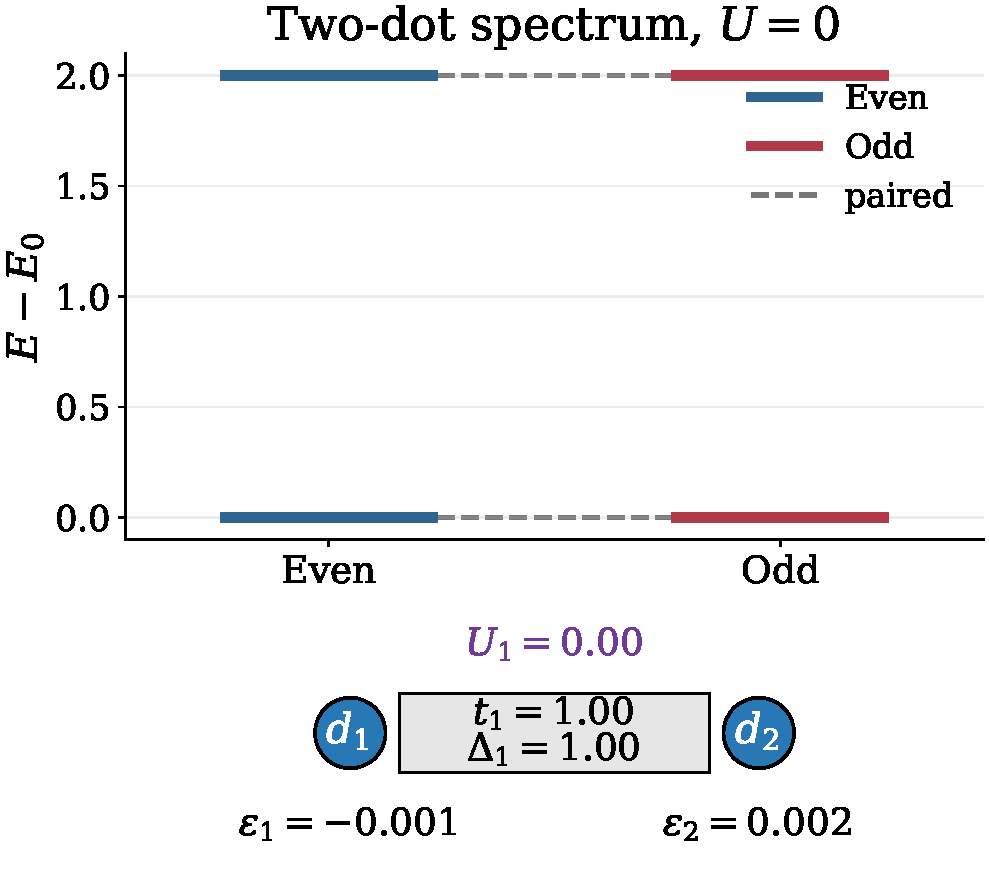
\includegraphics[width=0.49\textwidth]{figs/2DotU0.pdf}
  \hfill
  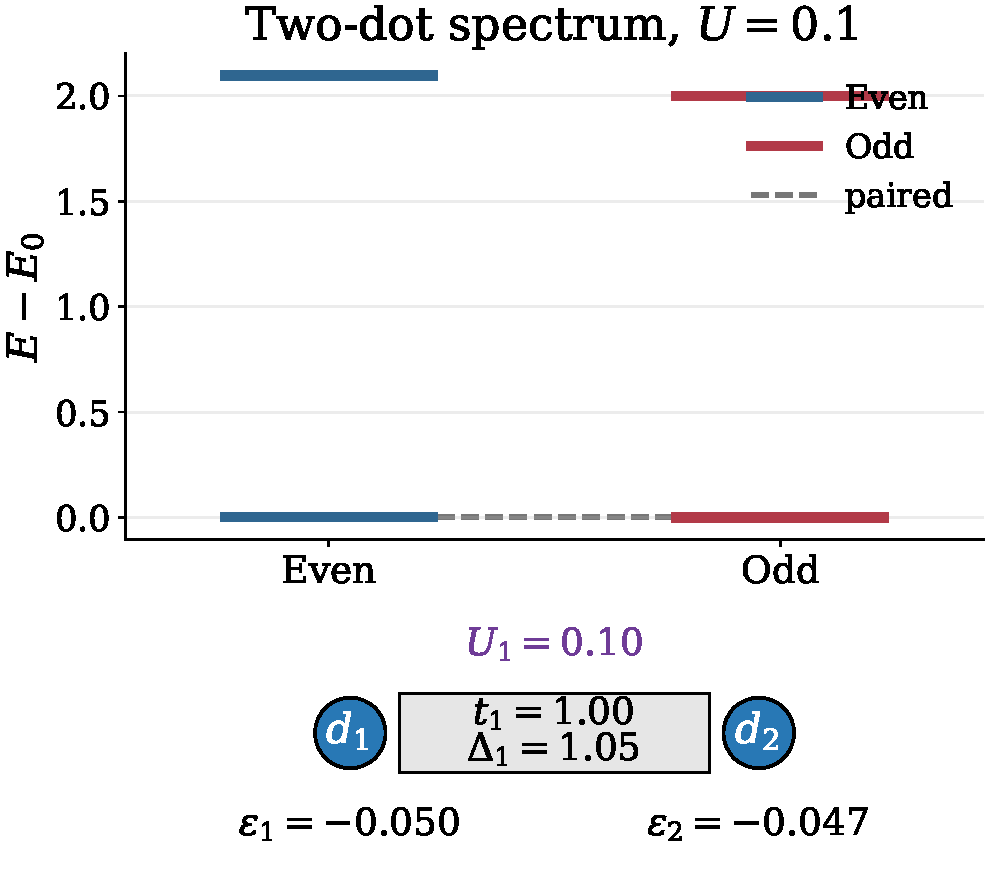
\includegraphics[width=0.49\textwidth]{figs/2DotU01.pdf}
  \caption{Parity-resolved spectra after optimization for the two-dot system at $U=0$ and $U=0.1$. Energies are shifted by the ground-state energy in each panel, and the optimized parameters are shown schematically below each spectrum.}
  \label{fig:2dot_schematicfirst}
\end{figure}

\begin{figure}[!htbp]
  \centering
  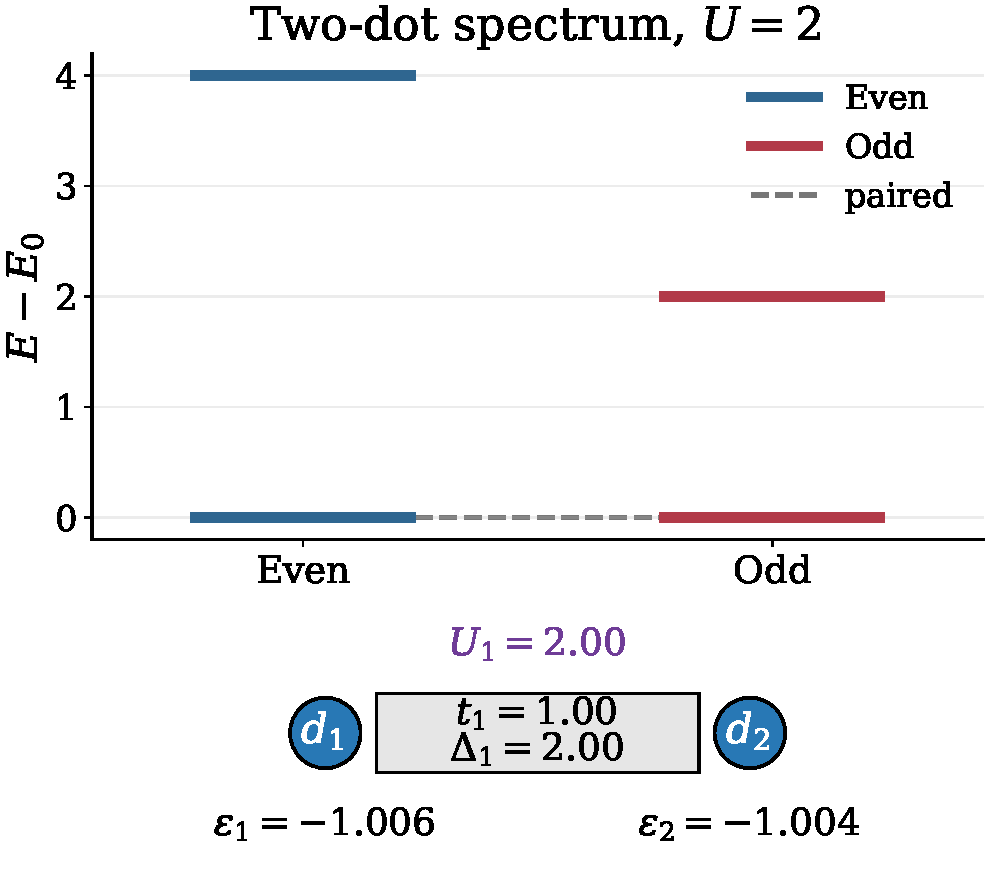
\includegraphics[width=0.74\textwidth]{figs/2DotU2.pdf}
  \caption{Parity-resolved spectrum after optimization for the two-dot system at $U=2.0$. Energies are shifted by the ground-state energy, and the optimized parameters are shown schematically below the spectrum.}
  \label{fig:2dot_schematicsecond}
\end{figure}
\newpage

The optimized three-dot system at $U=0.1$ provides a more promising
 configuration. As shown in Fig.~\ref{fig:3DotU01}, the
parity-resolved spectrum remains nearly paired, while the Majorana-polarization
profile has the expected edge-localized structure. The polarization is large
and opposite in sign on the two outer dots, and it is strongly suppressed on
the middle dot. This combination of spectral pairing and spatial Majorana
character motivates using this configuration as the main candidate for the
braiding calculations below. Comparing the three-dot and two-dot configurations at $U=0.1$ also illustrates how the additional site can help stabilize Majorana-like features in the presence of interactions. The excited-state degeneracy is better preserved in the three-dot case than in the two-dot case, even though both configurations have similar ground-state splitting and similar optimized parameters. The additional site therefore provides more freedom to optimize the excited states, which is important for maintaining a clean low-energy manifold that can support braiding.

\begin{figure}[!htbp]
  \centering
  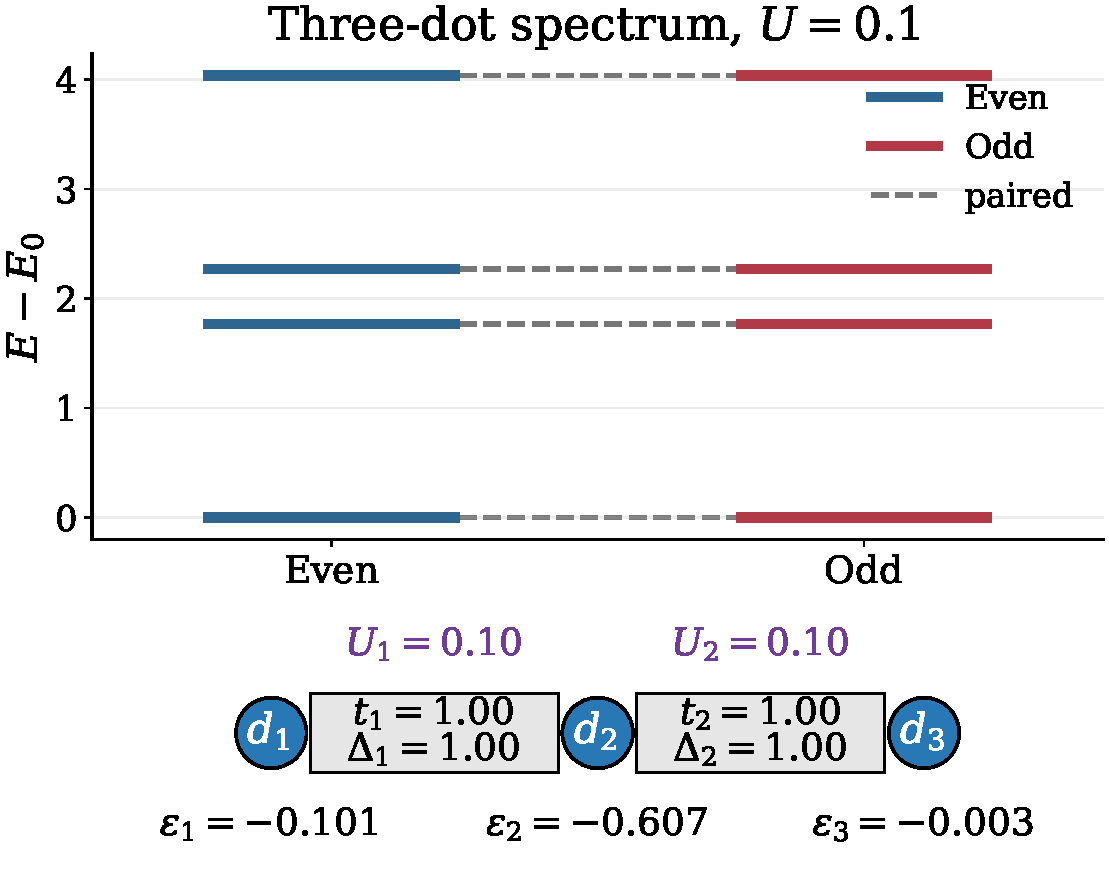
\includegraphics[width=0.55\textwidth]{figs/3DotU01.pdf}
  \hfill
  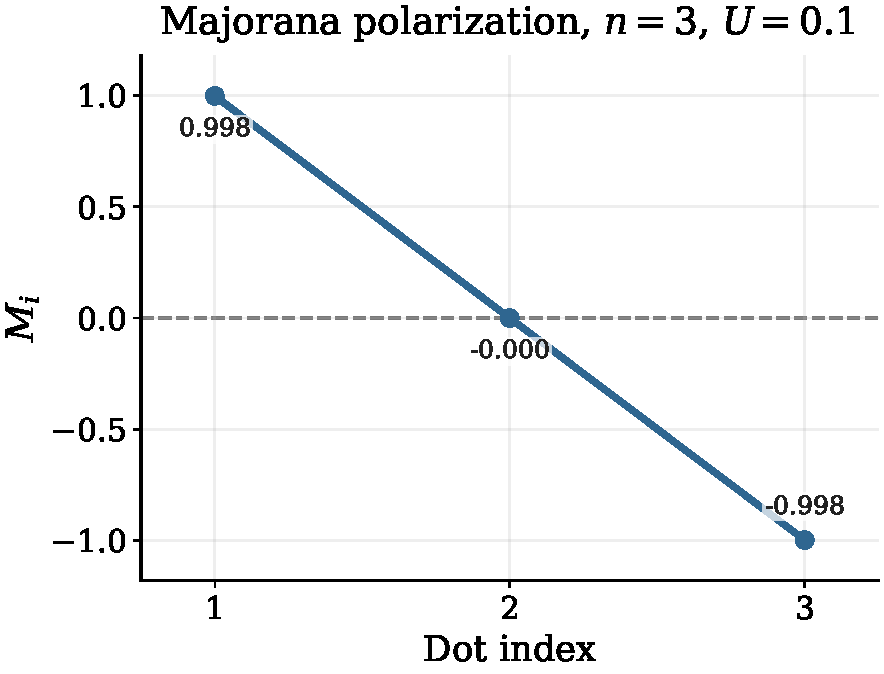
\includegraphics[width=0.41\textwidth]{figs/3DotMP01.pdf}
  \caption{Parity-resolved spectrum and Majorana-polarization profile for the optimized three-dot system at $U=0.1$. The left panel shows the optimized spectrum and parameters, while the right panel shows the Majorana polarization of the lowest even-odd pair.}
  \label{fig:3DotU01}
\end{figure}
\newpage

\section{Post-Optimization Diagnostics}
% The optimized parameter values alone do not determine whether a configuration is useful for Majorana braiding. 
After optimization, the candidate Hamiltonians must therefore be tested through spectral and local diagnostics. The parity-resolved spectra and low-energy gaps show whether the optimizer has produced an isolated nearly degenerate low-energy manifold, while the charge difference and Majorana-polarization profile test whether this manifold has the expected non-local and edge-localized Majorana character.

\subsection{Parity-resolved spectra and low-energy gaps}
\begin{figure}
  \centering
  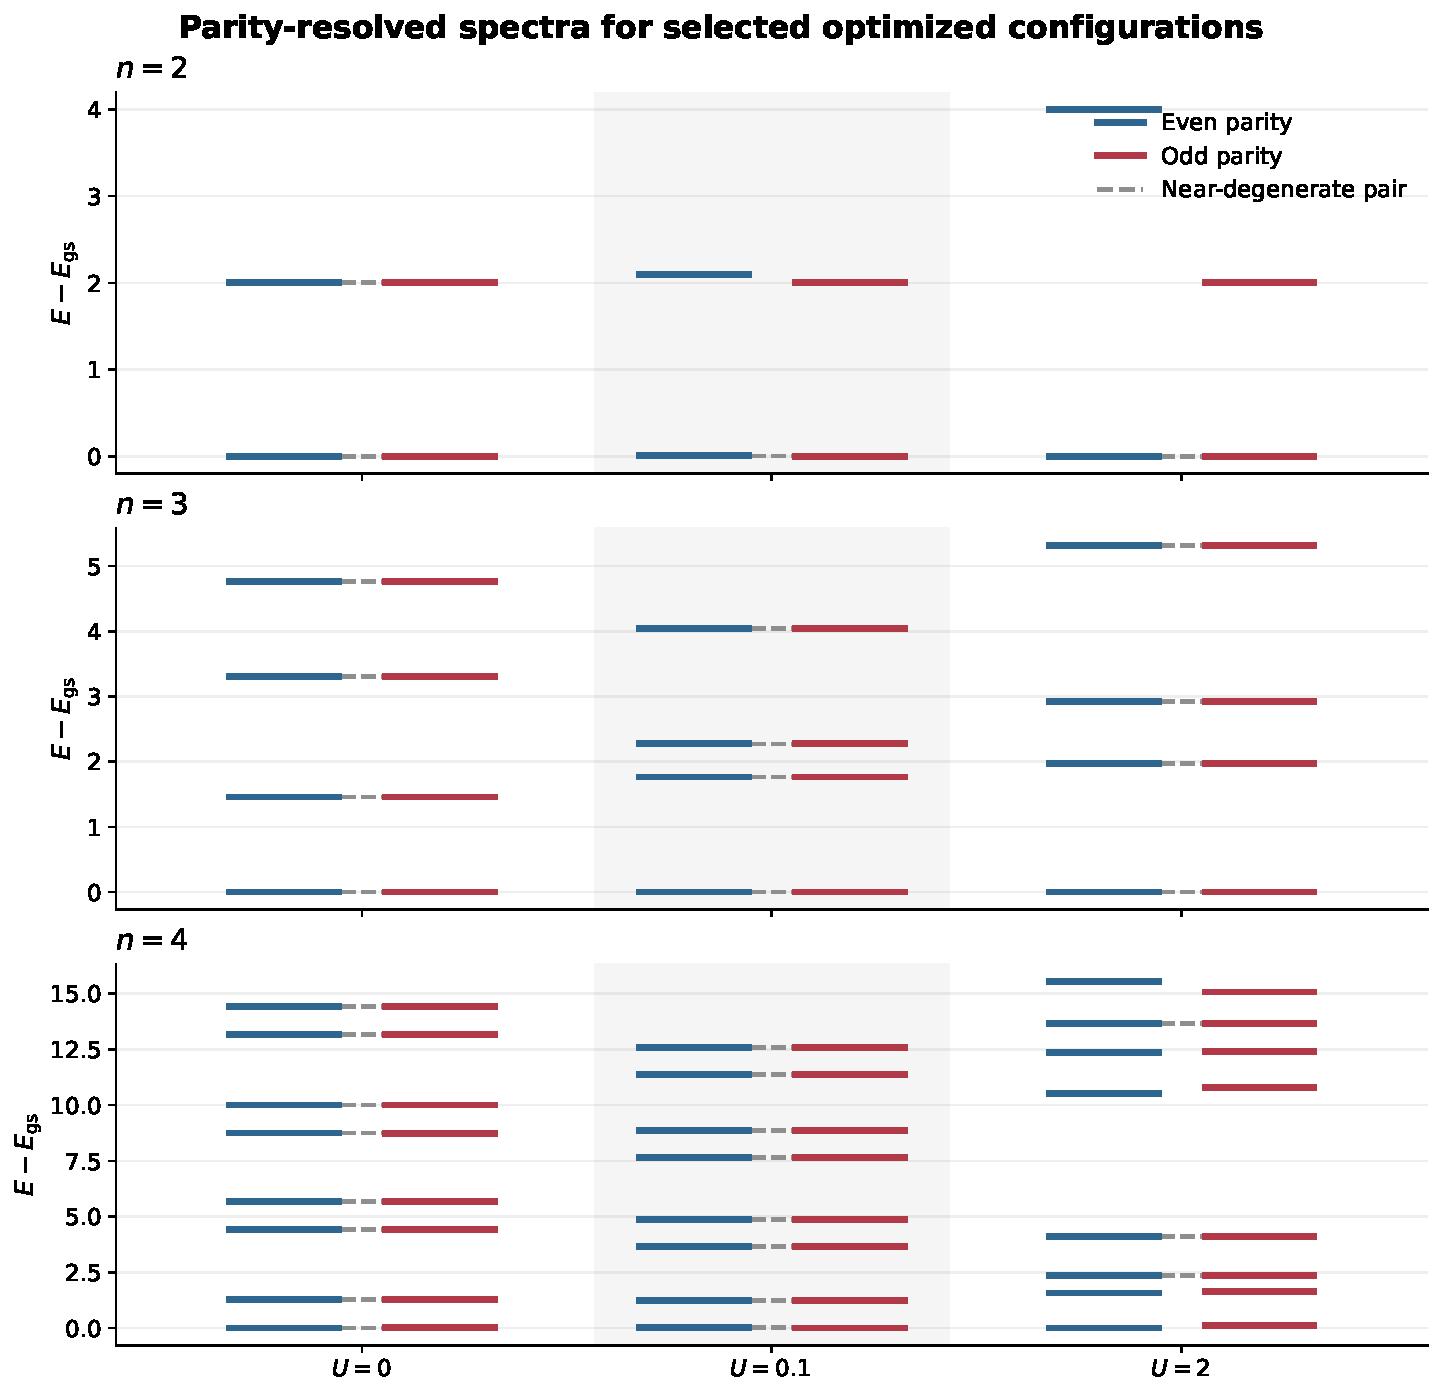
\includegraphics[width=\textwidth]{figs/parity_summary_u0_u01_u2.pdf}
  \caption{Parity-resolved spectra for the best optimized configurations at selected interaction strengths. Each panel corresponds to a different system size $n$, and energies are shifted so that the ground state is at zero.}
  \label{fig:parity_summary}
\end{figure}

Figure~\ref{fig:parity_summary} compares the parity-resolved spectra for $n=2,3,$ and $4$ at selected interaction strengths. A useful Majorana-like configuration should have a nearly degenerate lowest even-odd pair, together with a finite gap separating this pair from higher excited states. The dashed connectors in the figure indicate parity pairs that remain close in energy after optimization.

The non-interacting cases give the cleanest spectra, as expected. For the two-dot system, the parity pairing is nearly ideal at $U=0.0$, but the excited-state splitting becomes visible already at weak interaction and increases further at stronger interaction. 
% This shows that the interacting two-dot system can retain a low-energy degeneracy while losing clean parity pairing across the full finite spectrum.

The three-dot system is more stable across all interaction strengths shown, compared to both the two-dot and four-dot systems. For $U=0.0$, $U=0.1$, and $U=2.0$, the spectrum remains paired up to the numerical threshold, with relatively large gaps separating distinct energy sectors. The four-dot system shows a promising structure in the non-interacting and weakly interacting cases, while for the stronger interaction $U=2.0$ the energy degeneracy falls apart. Most importantly, the ground-state energies are no longer degenerate, so there is no longer a clear low-energy manifold that can support braiding. The three-dot system therefore appears to be the most robust candidate for maintaining a clean low-energy manifold across different interaction strengths, but the local diagnostics and Majorana character must also be checked before choosing it for braiding.

\subsection{Local diagnostics and Majorana character}
As discussed in the method chapter, Majorana-like states cannot be identified from spectral degeneracy alone. The parity-resolved spectra and low-energy gaps test whether the optimized Hamiltonian contains an isolated, nearly degenerate low-energy manifold. This subsection examines the complementary local diagnostics: the Majorana-polarization profile and the local charge difference between the lowest even-odd parity partners.

A convincing Majorana-like configuration should have opposite Majorana polarization on the two ends of the chain, with strongly suppressed polarization in the interior, as quantified by Eqs.~\ref{eq:method_edge_polarization} and~\ref{eq:method_bulk_polarization}. In addition, the even and odd parity partners should be locally difficult to distinguish. This is tested by the charge-difference diagnostic in Eq.~\ref{eq:method_charge_difference}, where smaller values indicate that the parity information is less visible to local charge measurements.

\begin{figure}[htbp]
  \centering
  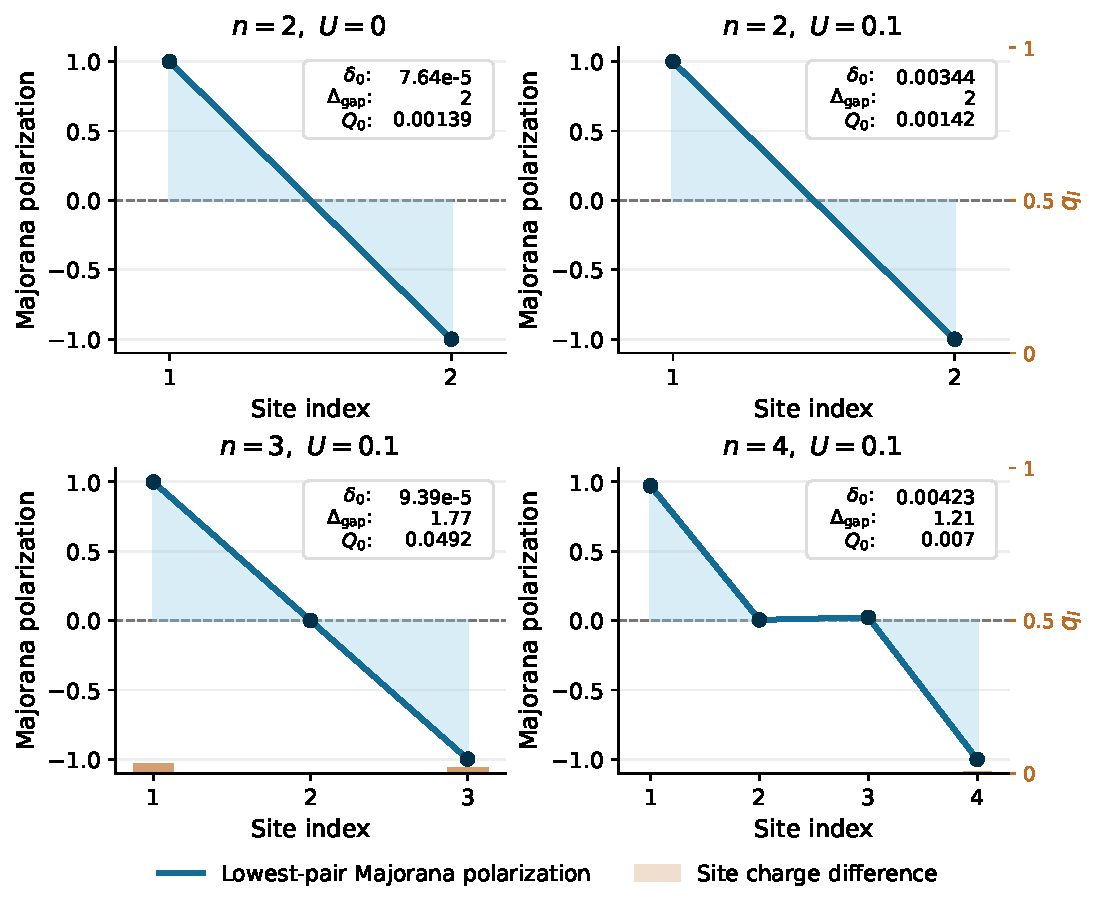
\includegraphics[width=0.95\textwidth]{figs/majorana_character_summary.pdf}
  \caption{Local diagnostics for representative optimized configurations. The blue curve shows the Majorana-polarization profile of the lowest even-odd pair, while the orange bars, read against the $0$--$1$ right axis, show the local charge difference $q_i=|\langle e | n_i | e \rangle - \langle o | n_i | o \rangle|$ on each site. The inset in each panel reports the ground-state splitting $\delta_0$, the low-energy gap $\Delta_{\mathrm{gap}}$, and the total charge difference $Q_0$.}
  \label{fig:majorana_character_summary}
\end{figure}
\newpage

\begin{table}
  \centering
  \begin{tabular}{c c c c c c c}
\hline
$n$ & $U$ & $\delta_0$ & $\Delta_{\mathrm{gap}}$ & $Q_0$ & $\overline{|M_{\mathrm{edge}}|}$ & $\max |M_{\mathrm{bulk}}|$ \\
\hline
2 & 0 & 7.64e-05 & 2 & 0.00139 & 1 & 0 \\
2 & 0.1 & 0.00344 & 2 & 0.00142 & 1 & 0 \\
3 & 0.1 & 9.39e-05 & 1.77 & 0.0492 & 0.998 & 0.000202 \\
4 & 0.1 & 0.00423 & 1.21 & 0.007 & 0.986 & 0.0233 \\
\hline
\end{tabular}

  \caption{Summary of local diagnostics for the representative configurations shown in Fig.~\ref{fig:majorana_character_summary}. Here $\delta_0$ is the splitting of the lowest even-odd pair, $\Delta_{\mathrm{gap}}$ is the gap separating this pair from the next excited states, $Q_0$ is the total charge difference between the parity partners, $\overline{|M_{\mathrm{edge}}|}$ is the mean absolute Majorana polarization on the first and last sites, and $\max |M_{\mathrm{bulk}}|$ is the largest absolute polarization on the interior sites.}
  \label{tab:majorana_character_summary}
\end{table}

Figure~\ref{fig:majorana_character_summary} compares the spatial profiles directly, while Table~\ref{tab:majorana_character_summary} summarizes the corresponding scalar diagnostics. For the two-dot system, the edge polarization is essentially ideal, with $\overline{|M_{\mathrm{edge}}|}\approx 1$ and no bulk contribution by construction. The total charge difference is also very small, $Q_0\approx 1.4\times 10^{-3}$, both at $U=0$ and at $U=0.1$. These two-dot cases are useful references, but because they have no interior sites they do not test suppression of Majorana weight in the bulk.

The three-dot configuration at $U=0.1$ gives the clearest interacting Majorana-polarization pattern. The ground-state splitting is only $\delta_0=9.39\times 10^{-5}$, the excitation gap remains large, $\Delta_{\mathrm{gap}}=1.77$, and the bulk polarization is almost completely suppressed, with $\max |M_{\mathrm{bulk}}|=2.02\times 10^{-4}$. Its charge difference, however, is larger than in the two-dot and four-dot reference cases, with $Q_0=0.0492$. This shows that the three-dot state is not ideal in every diagnostic, even though its spectral and polarization properties are the strongest.

The four-dot configuration at $U=0.1$ shows the opposite tradeoff. It has a smaller charge difference, $Q_0=0.0070$, and comparably strong edge polarization, $\overline{|M_{\mathrm{edge}}|}\approx 0.986$. However, the ground-state splitting increases to $\delta_0=4.23\times 10^{-3}$ and the bulk polarization rises to $\max |M_{\mathrm{bulk}}|=2.33\times 10^{-2}$.

Together, these diagnostics show that different system sizes optimize different aspects of the Majorana criteria. The four-dot case performs better in terms of local charge indistinguishability, while the three-dot case performs better in terms of spectral near-degeneracy and suppression of bulk Majorana weight. Since the braiding analysis requires a low-energy subspace that is both nearly degenerate and spatially well localized, the interacting three-dot system remains the most convincing candidate for the rest of the thesis.

\section{Selection of Braiding Candidate}
The braiding calculations are performed using the optimized three-dot configuration at $U=0.1$. This choice is based on the combined post-optimization diagnostics above. Although the four-dot configuration has a smaller local charge difference, the three-dot configuration has the most favorable combination of small ground-state splitting, large excitation gap, clear edge-localized Majorana-polarization profile, and strongly suppressed bulk polarization. Since the braiding analysis relies on a nearly degenerate and spatially localized low-energy subspace, the three-dot system is chosen as the main microscopic building block.

The optimized parameters used for each three-dot subsystem are
\begin{equation}
\Delta_1=1.001,\qquad
\Delta_2=1.002,\qquad
\epsilon_1=-0.101,\qquad
\epsilon_2=-0.607,\qquad
\epsilon_3=-0.003,
\end{equation}
with fixed hopping amplitudes $t_i=1$ and fixed interaction strength $U=0.1$.
 
In the braiding geometry, three identical copies of this optimized three-dot chain are combined. Each subsystem has Hilbert-space dimension $2^3=8$, giving a total microscopic Hilbert space of dimension $2^9=512$. This system is large enough to test braiding beyond the lowest projected manifold, while still being small enough for exact diagonalization and systematic sector-resolved scans. The selected configuration therefore provides a useful setting for studying how interactions affect braiding across the many-body spectrum.

\section{Braiding in the Ground-State Sector}
The optimized three-dot chain is now used as the building block for the braiding calculations. Before studying higher energy sectors, we first establish a controlled ground-state benchmark. The goal is to separate three related questions: whether the energy-level Majorana operators generate the expected exchange, whether projected microscopic junction couplings select the same exchange channel, and whether this channel is also visible through projected local endpoint operators.

The energy-level reference model generates the braid directly from tunable Majorana bilinears built from the four Majorana operators defined in Eq.~\ref{eq:four_majoranas}. This provides the clean baseline for the exchange protocol. In the projected microscopic junction model, these direct bilinears are replaced by projected junction operators constructed from the hopping and crossed-Andreev pairing Hamiltonian introduced in Eq.~\ref{eq:junctionHamiltonian}. After projection into the retained low-energy subspace, this gives the effective couplings \(T_{AB}\) and \(T_{AC}\) defined in Eq.~\ref{eq:method_projected_junctions}, which are used in the driven braid Hamiltonian of Eq.~\ref{eq:brajunc}. Finally, the projected local-operator model uses endpoint Majorana components instead of the full junction Hamiltonian, testing whether the same low-energy exchange channel is accessed by local microscopic operators.



\subsection{Energy-Level Majorana Reference}
\begin{figure}[htbp]
  \centering
  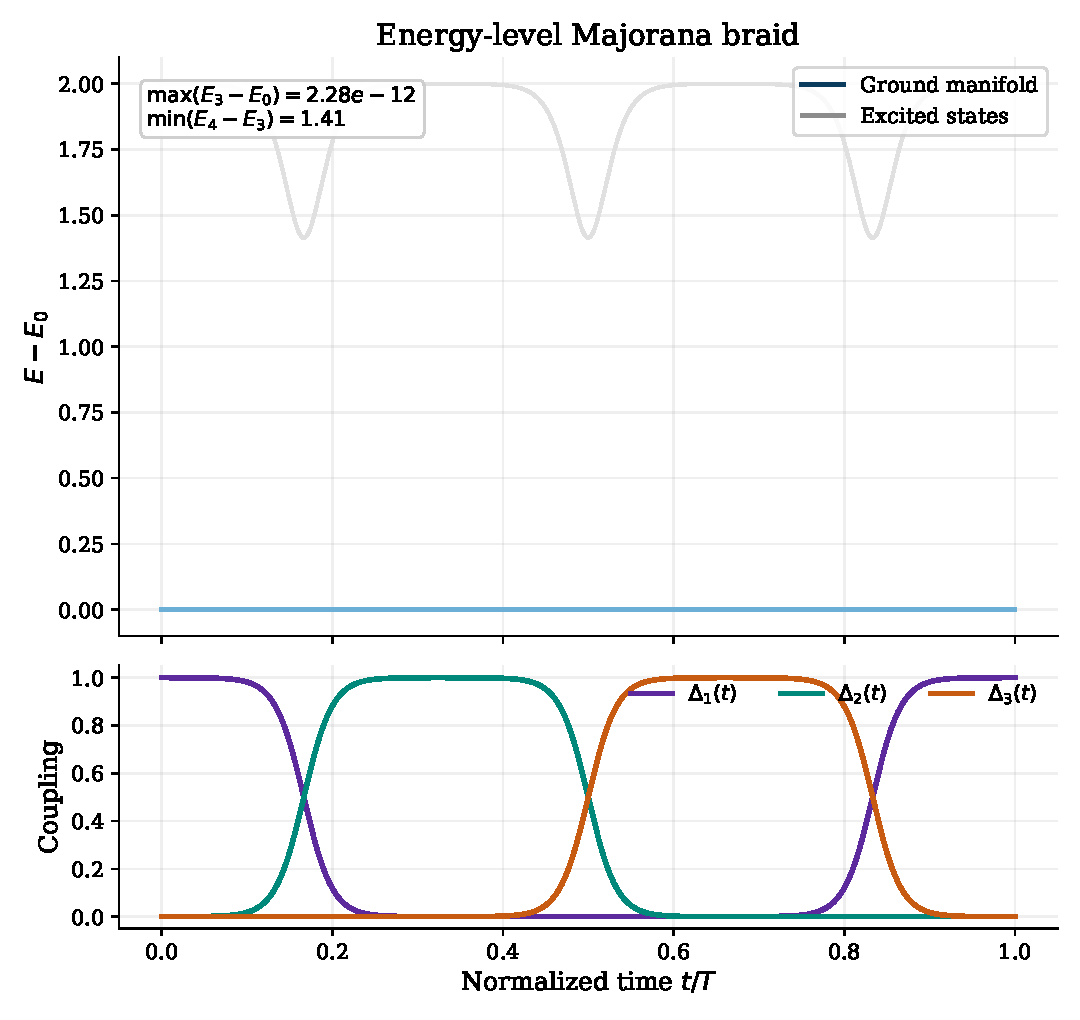
\includegraphics[width=0.9\textwidth]{figs/braiding_ideal_protocol.pdf}
  \caption{Energy-level Majorana braiding protocol. The top panel shows the instantaneous spectrum of the effective Hamiltonian during the braid, with all energies shifted so that the lowest state remains at zero. The bottom panel shows the three smooth pulse couplings that move the dominant Majorana coupling through the network.}
  \label{fig:braiding_ideal_protocol}
\end{figure}

Figure~\ref{fig:braiding_ideal_protocol} shows the reference braid generated by four active Majorana operators in the projected low-energy space. The three couplings are turned on sequentially, so that the dominant coupling is first between $\gamma_0$ and $\gamma_1$, then between $\gamma_0$ and $\gamma_2$, and finally between $\gamma_0$ and $\gamma_3$ before returning to the initial configuration. Throughout this cycle, the transported low-energy manifold remains essentially four-fold degenerate. The largest instantaneous splitting within this manifold is only $\max(E_3-E_0)=2.28\times 10^{-12}$, while the minimum gap to the excited states remains open at $\min(E_4-E_3)=1.414$.

Using Kato transport, the resulting unitary reproduces the expected single-exchange action on the Majorana operators. The largest error in the transformations $\gamma_2\rightarrow-\gamma_3$ and $\gamma_3\rightarrow\gamma_2$ is $3.34\times 10^{-6}$. In the parity-resolved gate blocks, the odd and even $2\times2$ blocks agree with the target exchange gate to within $6.53\times 10^{-8}$, while the off-block leakage is only $1.02\times 10^{-11}$. The effective model therefore provides a clean benchmark for the more microscopic projected calculations.

\newpage
\subsection{Projected Microscopic Junction Braid}
In this subsection we replace the direct Majorana-bilinear couplings from the previous subsection with the projected microscopic junction operators defined in Eq.~\ref{eq:method_projected_junctions}. The goal is to test whether it is possible to reproduce the same low-energy exchange channel using the junction Hamiltonian of Eq.~\ref{eq:junctionHamiltonian} instead of direct Majorana bilinears. This subsection identifies two separate findings. The first is which Majorana operators are actually being exchanged in the microscopic model. The second is whether this junction-based exchange can reproduce the target exchange channel of the energy-level reference model. 
\begin{figure}[htbp]
  \centering
  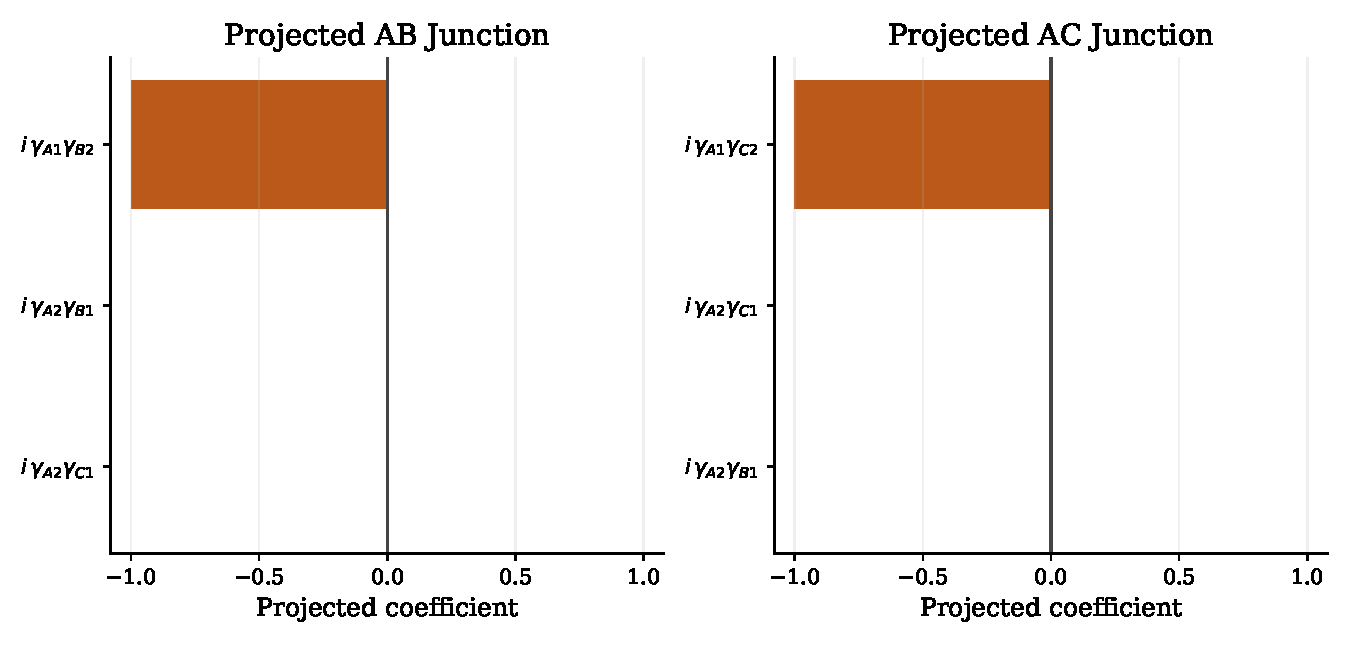
\includegraphics[width=0.95\textwidth]{figs/braiding_junction_decomposition.pdf}
  \caption{Dominant Majorana-bilinear components of the projected microscopic junction operators. The AB junction is almost entirely $i\gamma_{A1}\gamma_{B2}$, while the AC junction is almost entirely $i\gamma_{A1}\gamma_{C2}$. All subleading bilinears are strongly suppressed.}
  \label{fig:braiding_junction_decomposition}
\end{figure}

\Cref{fig:braiding_junction_decomposition} shows the decomposition of the projected junction terms $T_{AB}$ and $T_{AC}$ in the energy-level Majorana-bilinear basis. The AB junction is dominated by the bilinear $i\gamma_{A1}\gamma_{B2}$, while the AC junction is dominated by $i\gamma_{A1}\gamma_{C2}$. This identifies $\gamma_{B2}$ and $\gamma_{C2}$ as the Majoranas that participate in the microscopic braid, while $\gamma_{A1}$ acts as the shared Majorana through which the exchange is mediated. The remaining bilinear components are strongly suppressed, indicating that the junction Hamiltonian effectively selects a single low-energy exchange channel.  

\begin{figure}[htbp]
  \centering
  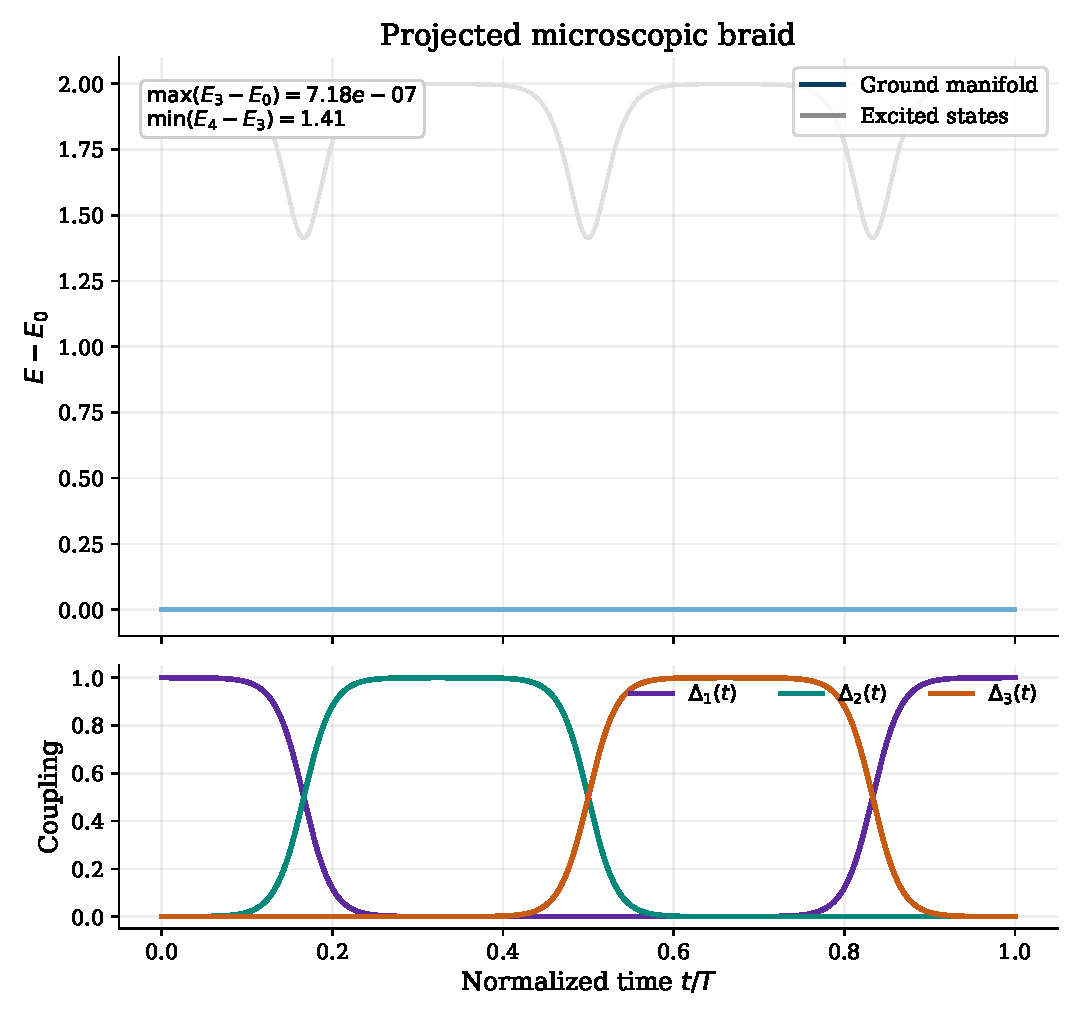
\includegraphics[width=0.9\textwidth]{figs/braiding_projected_protocol.pdf}
  \caption{Braiding protocol after replacing the direct reference couplings by projected microscopic junction operators. The spectral evolution remains almost identical to the energy-level benchmark, with a well-isolated low-energy manifold throughout the cycle.}
  \label{fig:braiding_junctionprotocol}
\end{figure}
\Cref{fig:braiding_junctionprotocol} shows the resulting braid after replacing the energy-level Majorana bilinears with the projected microscopic junction operators. The spectral evolution remains almost identical to the effective-model benchmark, with a well-isolated low-energy manifold throughout the cycle. The maximum splitting inside this manifold increases only to $\max(E_3-E_0)=7.18\times 10^{-7}$, while the minimum gap remains large, $\min(E_4-E_3)=1.413$.

\newpage
\subsection{Projected Local-Operator Braid}
The junction decomposition above identifies $\gamma_{B2}$ and $\gamma_{C2}$ as the active exchange channels. The next question is whether the same channels are obtained from local endpoint Majorana operators. For this, we use the projected local component
\[
\Gamma_{S,-}^{P}
=
\mathcal{N}_S V^\dagger \chi_{S,-}V,
\qquad
\chi_{S,-}=i(c_S^\dagger-c_S),
\]
corresponding to the \(\Gamma_-^P\) component introduced in Eq.~\ref{eq:local_gamma_ops}. The local-operator braid is then generated with the Hamiltonian of Eq.~\ref{eq:local_braid_ham}, using the same pulse sequence as in the energy-level and projected microscopic junction models.

\begin{table}[htbp]
  \centering
  \begin{tabular}{lcc}
\hline
Projected local operator & Dominant energy-level Majorana & Coefficient \\
\hline
$\Gamma_{B,\mathrm{L},-}^{P}$ & $\gamma_{B2}$ & -1.000 \\
$\Gamma_{B,\mathrm{R},-}^{P}$ & $\gamma_{B2}$ & 1.000 \\
$\Gamma_{C,\mathrm{L},-}^{P}$ & $\gamma_{C2}$ & -1.000 \\
$\Gamma_{C,\mathrm{R},-}^{P}$ & $\gamma_{C2}$ & 1.000 \\
\hline
\multicolumn{3}{l}{Endpoint consistency checks} \\
\hline
$B$ endpoints, $\chi_-$ component & opposite orientation & 8.969e-14 \\
$C$ endpoints, $\chi_-$ component & opposite orientation & 5.787e-14 \\
\hline
\end{tabular}

  \caption{Projected local endpoint operators used in the local-operator braid. The minus components project onto the same low-energy Majorana channels selected by the microscopic junction decomposition, $\gamma_{B2}$ and $\gamma_{C2}$, up to endpoint orientation.}
  \label{tab:braiding_local_projection}
\end{table}

\Cref{tab:braiding_local_projection} shows that the projected local minus components on the relevant endpoint sites select the same low-energy channels as the projected junction calculation. The left and right endpoint projections in subsystem $B$ both reduce to $\gamma_{B2}$, but with opposite orientation, and the same happens for subsystem $C$ and $\gamma_{C2}$. This sign only fixes the endpoint convention for the projected operator; the factor of $i$ is already contained in the definition of the minus component $\chi_-=i(c^\dagger-c)$.

\begin{figure}[htbp]
  \centering
  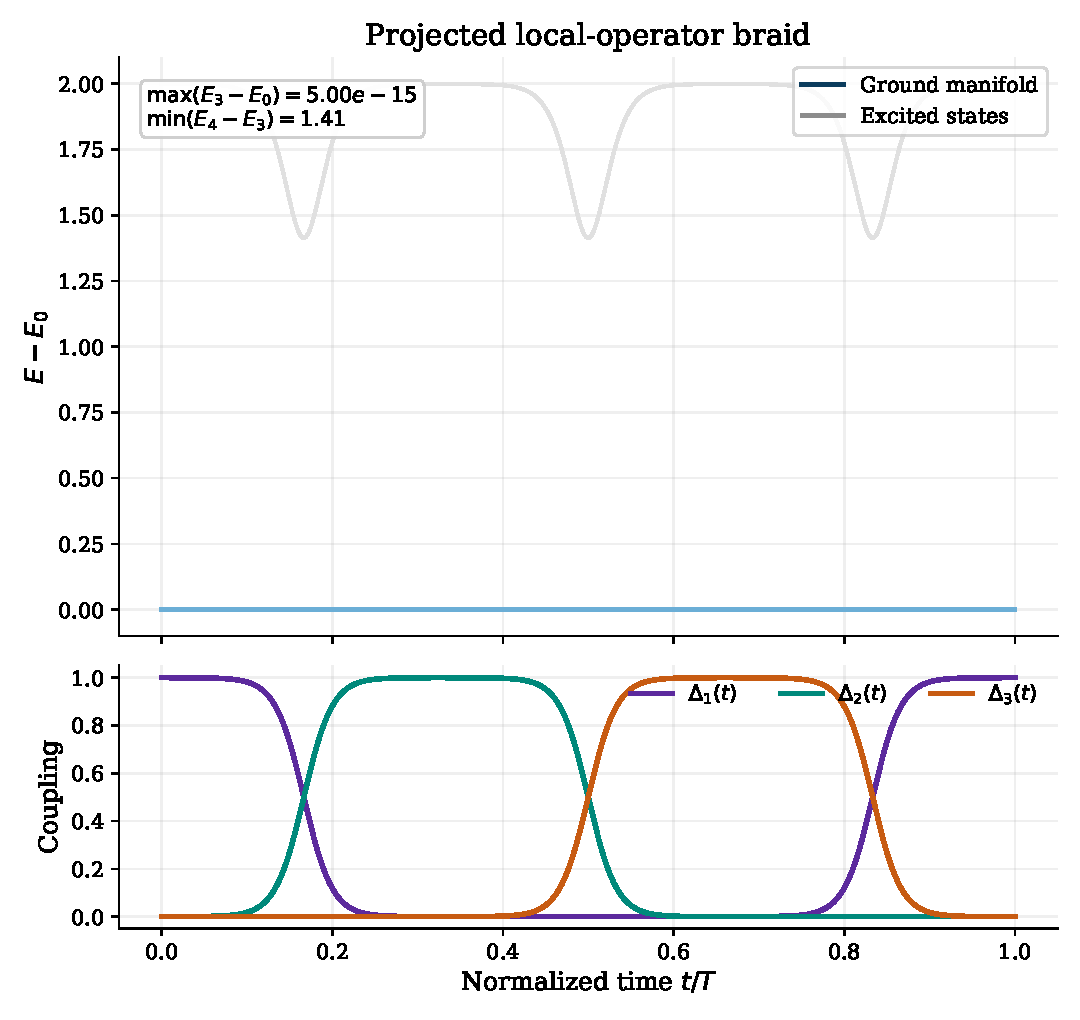
\includegraphics[width=0.9\textwidth]{figs/braiding_local_operator_protocol.pdf}
  \caption{Projected local-operator braiding protocol. The driven couplings follow the same pulse sequence as in the energy-level and projected microscopic junction models, but the exchanged operators are constructed from projected local endpoint Majorana components.}
  \label{fig:braiding_local_operator_protocol}
\end{figure}

\Cref{fig:braiding_local_operator_protocol} shows that the projected local-operator braid has the same stable low-energy structure as the two previous ground-sector braids. The transported four-dimensional manifold remains essentially degenerate, with $\max(E_3-E_0)=5.00\times10^{-15}$, while the gap to the excited states remains open at $\min(E_4-E_3)=1.414$.

\begin{table}[htbp]
  \centering
  \setlength{\tabcolsep}{5pt}
  \begin{tabular}{lcccccc}
\hline
Model & Split & Gap & 1x err. & Leakage & Odd err. & Even err. \\
\hline
Energy-level & 2.275e-12 & 1.414 & 3.343e-06 & 1.016e-11 & 6.527e-08 & 6.527e-08 \\
Projected junction & 7.175e-07 & 1.413 & 3.343e-06 & 8.727e-16 & 6.531e-08 & 6.531e-08 \\
Projected local & 4.996e-15 & 1.414 & 3.343e-06 & 7.542e-16 & 6.530e-08 & 6.530e-08 \\
\hline
\end{tabular}

  \caption{Comparison of the main braid diagnostics for the energy-level Majorana reference model, the projected microscopic junction model, and the projected local-operator model. Here ``Split'' denotes $\max(E_3-E_0)$, ``Gap'' denotes $\min(E_4-E_3)$, ``1x err.'' is the largest deviation in the expected single-exchange Majorana map, ``Leakage'' is the off-block norm in the parity basis, and the last two columns compare the odd and even parity blocks with the target exchange gate.}
  \label{tab:braiding_checks_comparison}
\end{table}

\Cref{tab:braiding_checks_comparison} shows that all three ground-sector braid constructions give essentially the same result. The maximum single-exchange error is $3.34\times10^{-6}$ in each case, the parity leakage remains below $10^{-11}$, and the odd- and even-parity blocks agree with the target exchange gate to approximately $6.5\times10^{-8}$. In the ground-state sector, the projected local endpoint operators therefore access the same exchange channel as the energy-level and microscopic junction constructions.

\newpage
\section{Braiding in Multiple Energy Sectors}
To explore whether braiding is possible beyond the lowest projected manifold, we first identify distinct energy sectors in the three-dot, three-subsystem system. This is done by combining the three single-subsystem Hamiltonians into one full-system Hamiltonian,
\begin{equation}
  H = H_A \otimes I_B \otimes I_C
  + I_A \otimes H_B \otimes I_C
  + I_A \otimes I_B \otimes H_C .
\end{equation}
This Hamiltonian captures the entire $2^9 \times 2^9$ Hilbert space of the Y-junction system. The three subsystems, $A$, $B$, and $C$, are initially decoupled and identical.

The full-system spectrum can then be grouped into distinct energy sectors. Each sector consists of states that are degenerate in energy, within the numerical tolerance, and separated by a gap from neighboring sectors, as shown in \cref{fig:full_hamil_elevels}.

\begin{figure}[htbp]
  \centering
  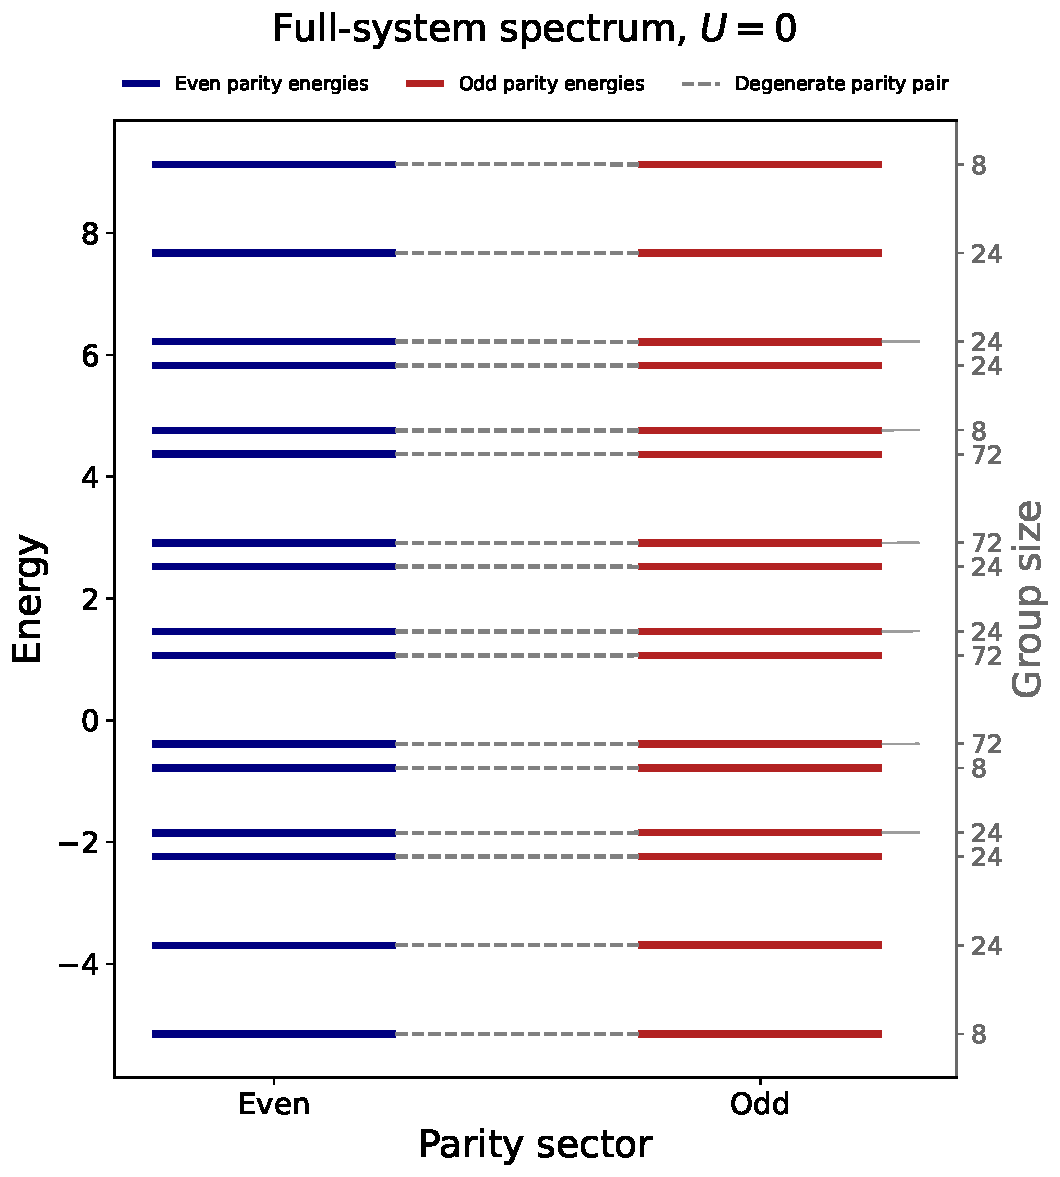
\includegraphics[width=0.9\textwidth]{figs/full_system_spectrum_U_0p0.pdf}
  \caption{Full-system Hamiltonian energy spectrum. The spectrum is split into even and odd eigenenergies. The dashed lines represent the degeneracy link between the even and odd sectors. The left-hand y-axis shows the energy levels, while the right-hand y-axis shows how many states reside in each energy sector. This figure was created for a single non-interacting system. Similar plots for the interacting model can be found in Appendix~\ref{app:energy_sectors}.}
  \label{fig:full_hamil_elevels}
\end{figure}

After the sectors have been identified, the same braid protocol can be applied sector by sector. For sector $i$, we form a sector basis $V_i$ from the eigenvectors belonging to that sector, and operators are represented in the selected space as $V_i^\dagger O V_i$, as described in \cref{eq:method_operator_projection}. This makes it possible to test whether each braid construction produces its intended exchange behavior beyond the lowest projected manifold.

The sector bases have different dimensions. For example, the ground-state sector contains $8$ states inside the full $512$-dimensional Hilbert space, while the first excited sector contains $24$ states. When the braid couplings are activated, the selected sector splits into a lower and an upper band of equal dimension, separated by a gap, as shown in \cref{fig:level_split}. This split provides a well-defined lower band for Kato transport, but does not by itself establish that the resulting unitary performs a successful Majorana exchange. The target-overlap deviation \(D_{\mathcal{O}}=|1-\mathcal{O}|\), defined in \cref{eq:method_overlap_deviation}, provides that separate test.

For the sector-resolved scans, the transported dimension was therefore fixed to half of the selected sector dimension, as defined in \cref{eq:method_sector_transport_dimension}. In each sector, the Kato calculation transports the lower band and measures whether its final unitary reproduces the intended exchange. The scans below are self-target comparisons: each braid construction is compared with its own target operator. Agreement between the projected local and energy-level exchange channels requires the separate common-target comparison discussed in the method section.

\begin{figure}[htbp]
  \centering
  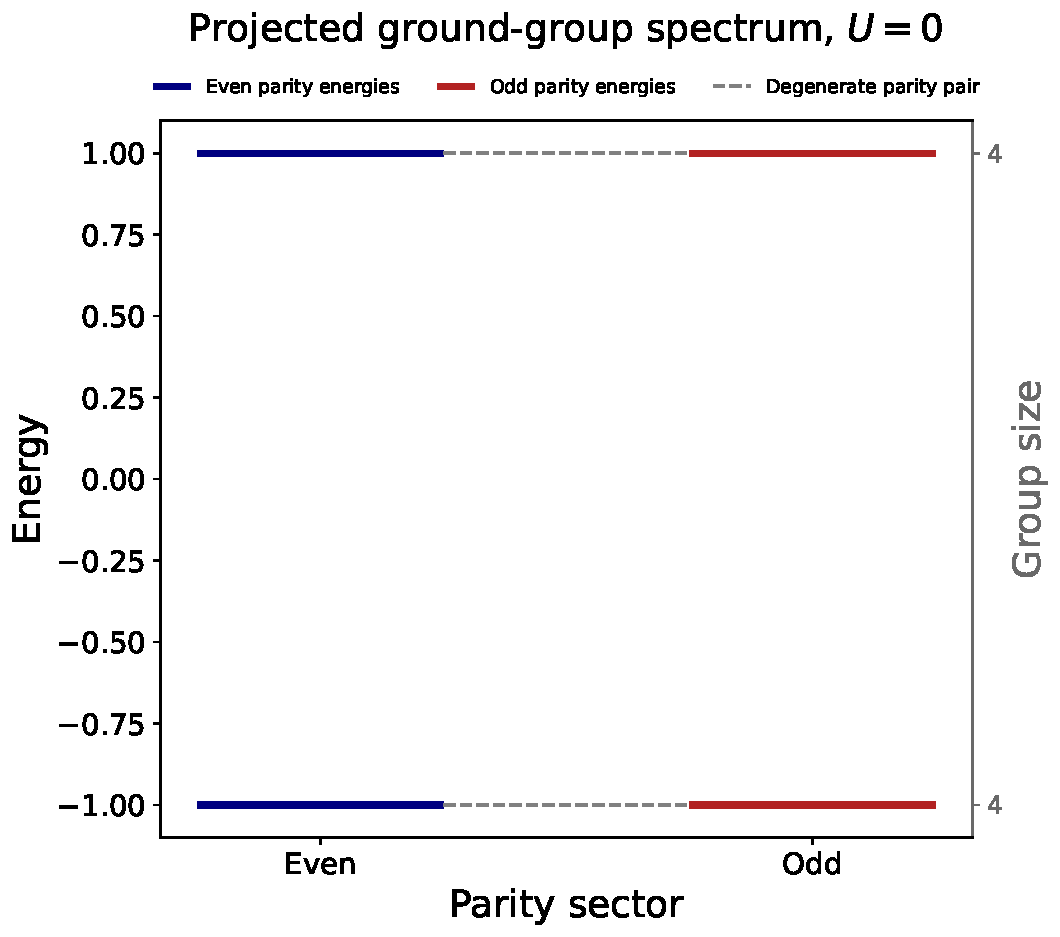
\includegraphics[width=0.9\textwidth]{figs/projected_ground_group_spectrum_U_0p0.pdf}
  \caption{Splitting of an initially degenerate energy sector into two distinct bands when the braid Hamiltonian is initialized. This representative example is the ground-state sector of the projected local-operator braid in the non-interacting system.}
  \label{fig:level_split}
\end{figure}



The first scan provides an energy-level Majorana baseline, starting with the ground-state sector and then moving through the higher energy sectors while simultaneously checking different interaction strengths. In this construction, the Majorana operators are built directly from paired even and odd eigenstates of each optimized subsystem. The non-interacting case provides the cleanest reference, while the interacting cases test whether the energy-level exchange channel extracted from the optimized spectra remains stable across sectors.
\begin{figure}[htbp]
  \centering
  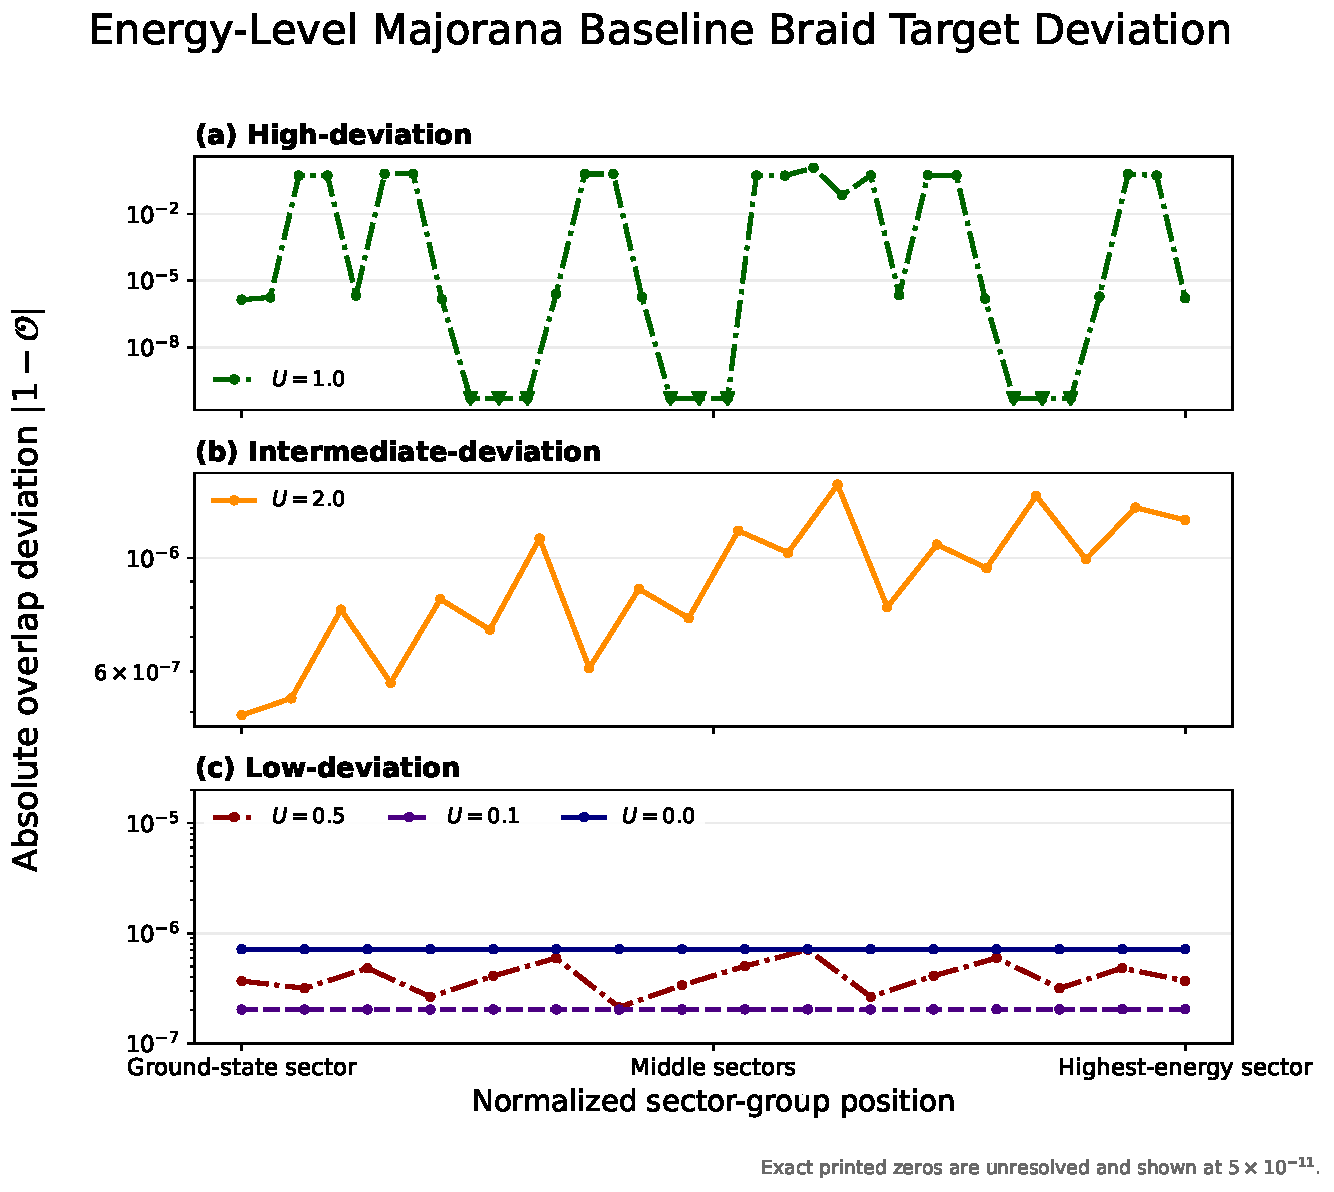
\includegraphics[width=0.9\textwidth]{figs/ideal_operator_interaction_regimes.pdf}
  \caption{Self-target braid errors for the energy-level Majorana baseline across different energy sectors and interaction strengths $U=0.0$, $U=0.1$, $U=0.5$, $U=1.0$, and $U=2.0$, plotted as the overlap deviation \(D_{\mathcal{O}}=|1-\mathcal{O}|\). The figure is split into three deviation regimes: a) $U=1.0$, b) $U=2.0$, and c) $U=0.0$, $U=0.1$, and $U=0.5$. The energy-level construction supports accurate braiding across all sectors for the non-interacting and weakly interacting configurations, while the $U=1.0$ configuration shows strong sector-dependent failures.}
  \label{fig:ideal_operator_interaction_regimes}
\end{figure}
\newpage
\Cref{fig:ideal_operator_interaction_regimes} displays the energy-level Majorana baseline. Here the $\gamma$ operators are created directly from the paired eigenstates by the construction $\gamma=\ket{e}\bra{o}+\mathrm{h.c.}$ before being projected into each sector and placed in the braid Hamiltonian. The high-deviation panel shows that the $U=1.0$ configuration is strongly sector dependent, as some sectors remain accurate, while others have errors of order $10^{-1}$. The $U=2.0$ results are much more stable across sectors and generally lie around $10^{-6}$. For $U=0.0$, $U=0.1$, and $U=0.5$, the errors remain below the $10^{-6}$ threshold across all sectors. The unusually poor and irregular $U=1.0$ result, despite the stronger $U=2.0$ configuration performing better in this baseline, shows that interaction strength alone does not necessarily explain the ordering of the selected configurations.



Since the low-energy junction decomposition identifies $\gamma_{B2}$ and $\gamma_{C2}$ as the active exchange channels, the projected local-operator model uses the minus endpoint components in subsystems $B$ and $C$,
\begin{equation}
  \Gamma_{S,-}^{(i)}
  =
  \mathcal{N}_{S,i}V_i^\dagger \chi_{S,-}V_i,
  \qquad
  \chi_{S,-}=i(c_S^\dagger-c_S),
  \qquad
  S=B,C.
\end{equation}
When these local operators are compared with $\gamma_{B2}$ and $\gamma_{C2}$, only an overall plus or minus sign is allowed.

\begin{figure}[htbp]
  \centering
  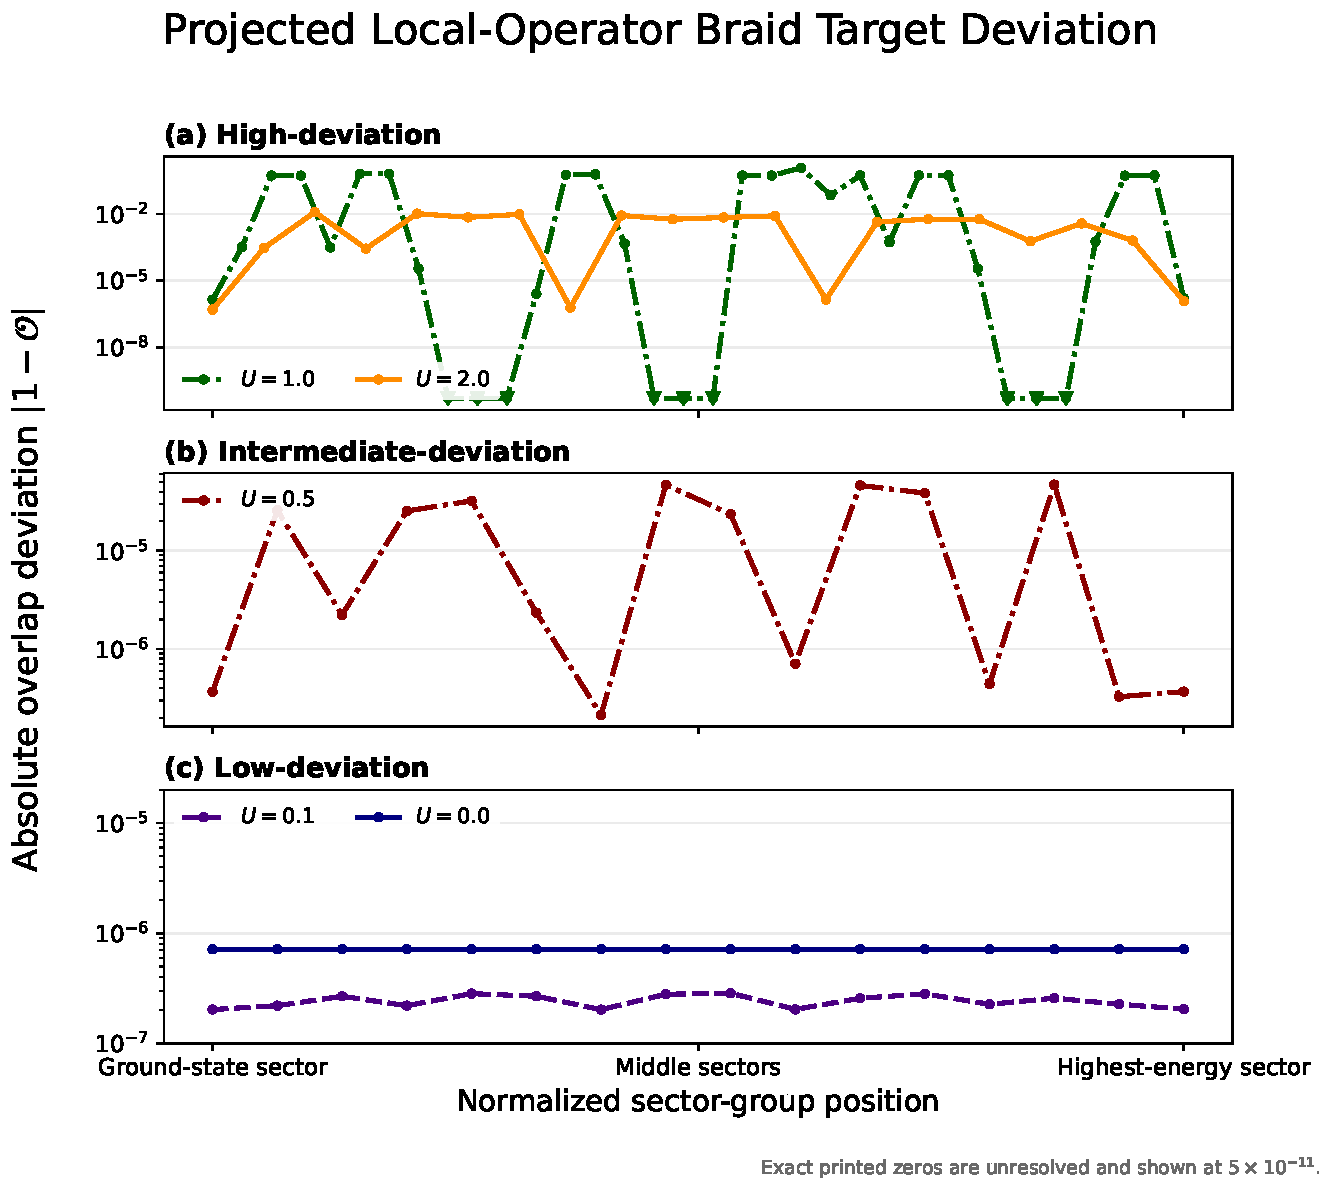
\includegraphics[width=0.9\textwidth]{figs/projected_operator_interaction_regimes.pdf}
  \caption{Self-target braid errors for the projected local-operator model across different energy sectors and interaction strengths $U=0.0$, $U=0.1$, $U=0.5$, $U=1.0$, and $U=2.0$, plotted as the overlap deviation \(D_{\mathcal{O}}=|1-\mathcal{O}|\). The figure is split into three deviation regimes: a) $U=1.0$ and $U=2.0$, b) $U=0.5$, and c) $U=0.0$ and $U=0.1$. The selected weak-interaction configurations have low deviations across all sectors, while the selected stronger-interaction configurations contain sectors with larger self-target errors.}
  \label{fig:projected_operator_interaction_regimes}
\end{figure}
\Cref{fig:projected_operator_interaction_regimes} shows how the self-target braid errors vary among the projected local-operator configurations. The high-deviation panel shows that the selected $U=1.0$ and $U=2.0$ configurations contain sectors with errors as large as order $10^{-1}$ and $10^{-2}$, respectively. Compared with the energy-level Majorana baseline in \cref{fig:ideal_operator_interaction_regimes}, the $U=0.5$ configuration is also more sensitive to sector choice in the projected local-operator model, with errors reaching approximately $10^{-5}$. For $U=0.0$ and $U=0.1$, the errors remain below $10^{-6}$ across all tested sectors. However, because each interaction strength uses a separately optimized parameter set, this trend does not isolate interaction strength as the sole cause.


During the scans, many higher-dimensional energy sectors were found to contain several internal blocks. For example, a $24$-dimensional sector can contain three independent $8\times8$ blocks, as illustrated in \cref{fig:24x24maj}. This matters because a projected local operator does not necessarily have one global orientation across the full sector. In some sectors, the local operator can be fitted to the energy-level Majorana operator with one overall sign across all blocks. In others, different blocks select different relative signs.

To account for this structure, we use the block-matched local-operator model described in \cref{eq:method_block_matched_majorana} and \cref{app:block_label_method}. Each sector scan first fits the projected local operators independently within the labelled blocks. The fitted blocks are then reassembled into one operator on the full sector and used in the braid Hamiltonian.
\begin{figure}[htbp]
  \centering
  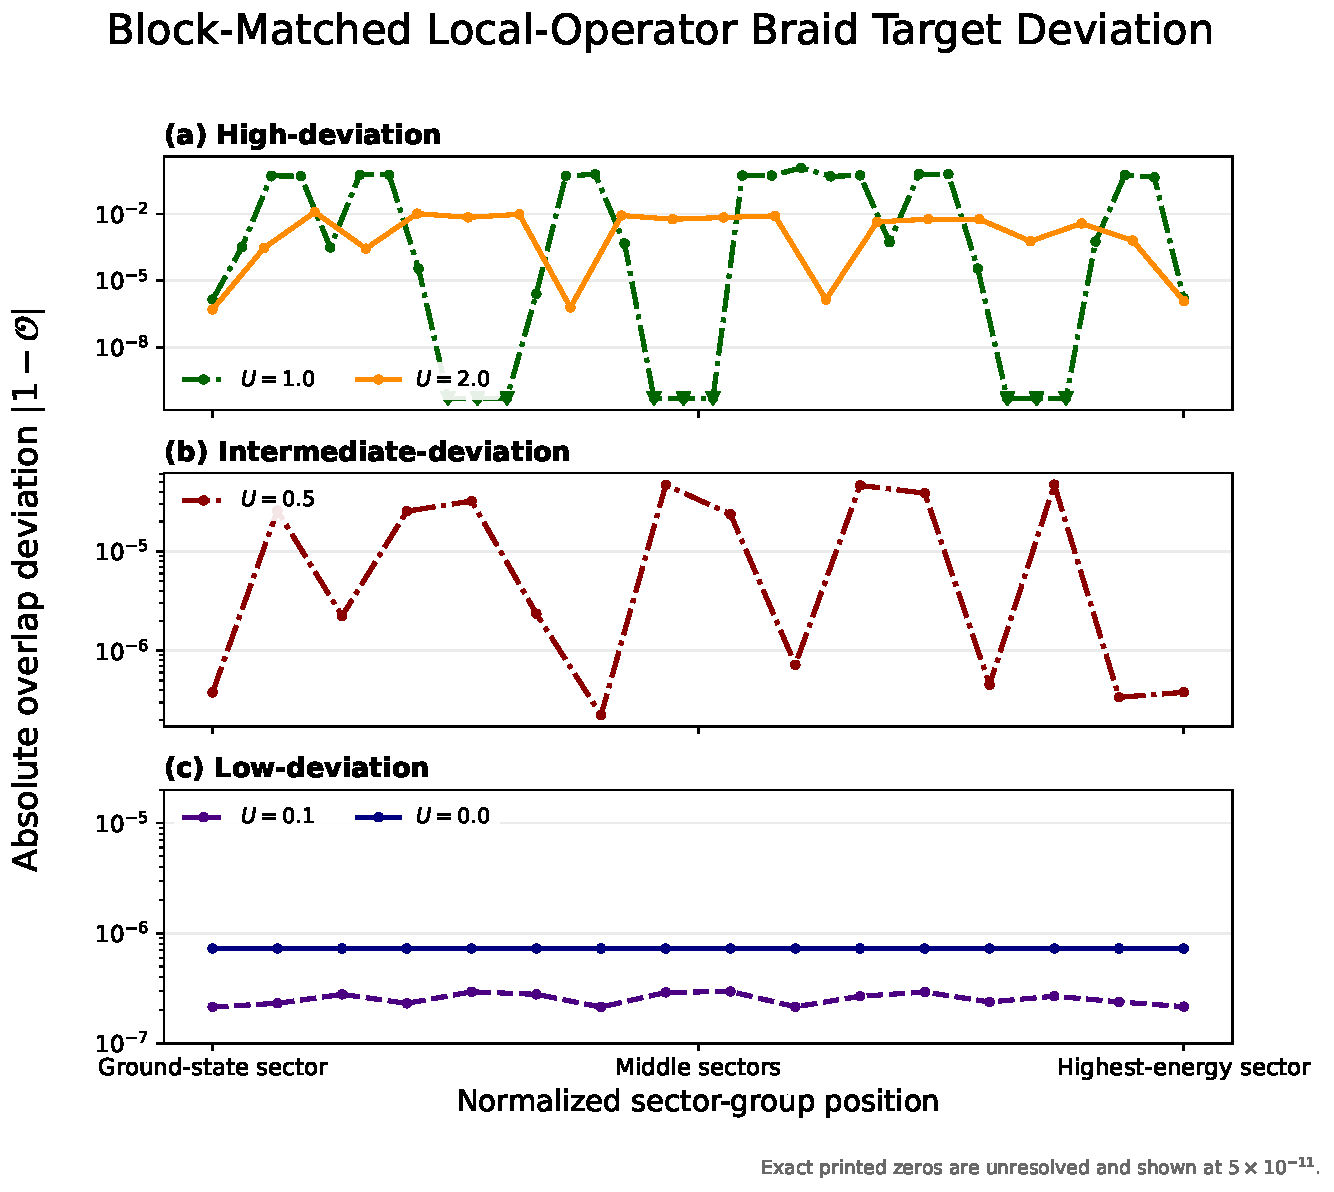
\includegraphics[width=0.9\textwidth]{figs/matched_operator_interaction_regimes.pdf}
  \caption{Self-target braid errors for the block-matched local-operator model, plotted as the overlap deviation \(D_{\mathcal{O}}=|1-\mathcal{O}|\). The same three deviation regimes as in \cref{fig:projected_operator_interaction_regimes} remain visible: a) $U=1.0$ and $U=2.0$, b) $U=0.5$, and c) $U=0.0$ and $U=0.1$.}
  \label{fig:matched_operator_interaction_regimes}
\end{figure}

\Cref{fig:matched_operator_interaction_regimes} shows that the block-matched construction retains the same overall self-target error regimes as the direct projected local-operator model. The $U=0.0$ and $U=0.1$ configurations remain accurate across the tested sectors, while the deviations increase at $U=0.5$ and become larger and more sector dependent for $U=1.0$ and $U=2.0$. Resolving and independently fitting the internal blocks therefore does not by itself remove the sensitivity observed in the local-operator construction.

The resulting blockwise coefficients are reported in \cref{tab:matched_operator_coefficients}. The numerical fitting errors remain between approximately $10^{-15}$ and $10^{-13}$ across all tested interaction strengths, showing that the block-matched operators reproduce the projected local operators essentially exactly. The first-component coefficients are strongly suppressed, so the local endpoint operators remain aligned with the intended second Majorana component rather than rotating into a different energy-level Majorana direction. For $U=0.0$ and $U=0.1$, the fitted second-component coefficients are close to $\pm1$ across all blocks. Small deviations become visible at $U=0.5$, while $U=1.0$ and $U=2.0$ show larger block-dependent variations in magnitude.

The coefficient table also reveals that different blocks within the same sector can select different relative exchange orientations. Since the first-component coefficients vanish at the saved precision, the blockwise braid is controlled mainly by the sign of the product $b_{B,r}b_{C,r}$, as explained in \cref{app:matched_operator_coefficients}. A sector containing both signs does not implement one uniform exchange orientation relative to the energy-level convention. Instead, its fitted target is a direct sum of block-dependent exchange orientations. The individual signs depend on the chosen Majorana sign convention, but their blockwise pattern records how the projected local channels are oriented relative to the fixed energy-level construction.

\begin{figure}[htbp]
  \centering
  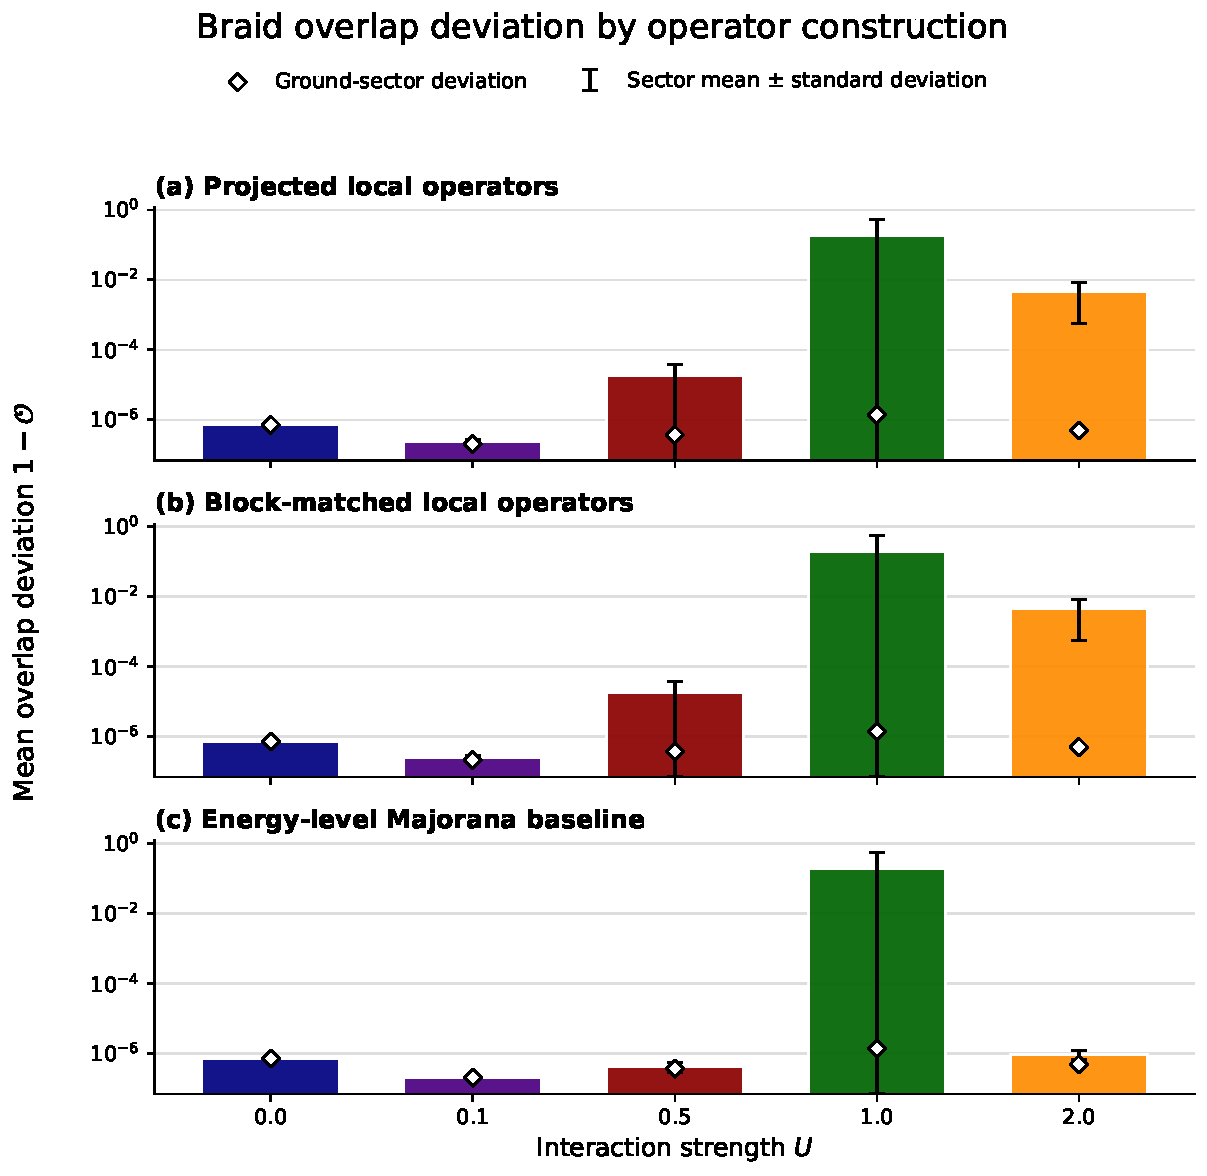
\includegraphics[width=0.9\textwidth]{figs/step_projection_mean_comparison.pdf}
  \caption{Mean self-target braid error across the tested sectors for a) the projected local-operator model, b) the block-matched local-operator model, and c) the energy-level Majorana baseline, using the overlap deviation \(D_{\mathcal{O}}=|1-\mathcal{O}|\). The ground-sector error is marked by a white diamond, and the standard deviation across sectors is shown by a black bar.}
  \label{fig:mean_braid_errors}
\end{figure}
\Cref{fig:mean_braid_errors} summarizes the sector-resolved self-target errors for the projected local-operator model, the block-matched local-operator model, and the energy-level Majorana baseline. For each interaction strength, the bar shows the unweighted mean across the identified sectors, the white diamond marks the ground-sector error, and the black bar shows the sector-to-sector standard deviation. Within these respective target comparisons, the $U=0.1$ and $U=0.0$ configurations have the lowest mean deviations. At $U=0.5$, the local-operator constructions show a noticeable increase in their mean errors, while the energy-level Majorana baseline remains accurate. The worst and most sector-dependent performance occurs at $U=1.0$, while $U=2.0$ is accurate in the energy-level baseline but less accurate in both local-operator constructions.

\newpage
\section{Summary of Main Findings}

The optimization study shows that the PMM chains recover the expected limits while also producing nontrivial interacting configurations. For the non-interacting two-dot system, the optimizer reproduces the known sweet spot, with nearly degenerate parity pairs and edge-localized Majorana polarization. For longer chains, the optimized parameters become increasingly inhomogeneous. In particular, the interior onsite energies are often shifted more strongly than the edge onsite energies. This interior detuning is correlated with favorable edge-localization diagnostics.

The post-optimization diagnostics identify the three-dot system at $U=0.1$ as the strongest interacting braiding candidate. This configuration combines a small ground-state splitting, a large excitation gap, strong opposite-sign edge Majorana polarization, and strongly suppressed bulk polarization. The four-dot system gives a smaller charge difference in the representative weakly interacting case, but it also shows larger ground-state splitting and stronger bulk polarization. Among the tested configurations, the three-dot system therefore provides the best overall compromise between spectral degeneracy and spatial localization. It also decreases the computational cost of the sector-resolved braiding calculations compared with the four-dot system.

The low-energy braiding calculations support this choice. After projection to the lowest manifold, the optimized three-dot building block reproduces the energy-level Majorana operator exchange with high accuracy. The projected microscopic junction operators are dominated by the intended Majorana bilinears, and the energy-level Majorana reference model, the projected microscopic junction model, and the projected local-operator model give nearly identical braid diagnostics in the lowest projected space. This shows that the optimized interacting PMM system can realize the expected Majorana exchange within the controlled low-energy projected model.

Within their respective target comparisons, the sector-resolved scans show low self-target braid errors across all identified energy sectors for the non-interacting and weakly interacting configurations. The energy-level Majorana baseline remains stable for $U=0.0$, $U=0.1$, $U=0.5$, and $U=2.0$, while the selected $U=1.0$ configuration shows large variations between sectors. The direct and block-matched local-operator models are more sensitive in their self-target errors, as these errors increase already at $U=0.5$, and both $U=1.0$ and $U=2.0$ contain less accurate sectors.

The block-matching analysis shows that the projected local operators can be represented essentially exactly within the energy-level Majorana basis. Within each block, the local endpoint operator remains aligned with the intended second Majorana component, while its magnitude and sign can vary between blocks. The relative signs of the two exchanged operators determine whether a block follows the same or opposite exchange orientation relative to the fixed energy-level convention. A sector containing both orientations therefore does not implement one uniform logical exchange across all its internal blocks. Despite resolving this structure, block matching does not substantially change the self-target braid deviations relative to the direct projected local-operator model.

The especially poor and irregular $U=1.0$ result should therefore be treated as a property of the selected optimized configuration, not as evidence that $U=t=1$ is generally worse for braiding than $U=2t$.

For configurations that support a stable exchange channel, the self-target braid accuracy is relatively insensitive to the chosen energy sector. However, the strongly sector-dependent $U=1.0$ result shows that this behavior is not guaranteed and depends on the selected optimized configuration. The differing sector dependence of the energy-level and local constructions leaves a common-target comparison as an important next check before drawing conclusions about how accurately a projected local channel accesses the energy-level exchange.

% \section{Results and Physical Interpretation}
This chapter presents the main numerical results of the thesis and discusses their physical meaning. I first report the outcome of the parameter optimization, then analyze the spectral and local signatures of the optimized configurations, and finally study whether the resulting low-energy states support the intended braiding behavior. The emphasis is not only on which parameter sets minimize the loss function, but also on whether those configurations can be interpreted as physically meaningful Majorana-like regimes.

\subsection{Parameter Optimization Results}
To obtain an overview of the optimization landscape, I first compare the lowest-loss configuration found for each combination of system size $n$ and fixed interaction strength $U$. This separates the global trends of the optimization procedure from the more detailed diagnostics of individual configurations. For the two-dot system, the optimizer reproduces the known non-interacting sweet spot at $U=0$, while increasing interaction strength gradually shifts the optimal on-site energies and pairing amplitudes away from that limit. For three and four dots, the optimization landscape becomes more complex, and the best solutions show stronger inhomogeneity in both the onsite energies and the pairing amplitudes.


\subsubsection{Dependence on interaction strength and system size}
Table \ref{tab:best_optimized_configs} summarizes the lowest-loss configuration found for each combination of system size $n$ and fixed interaction strength $U$. Since the hopping amplitudes were fixed to $t_i = 1$ in these runs, only the optimized pairing amplitudes and on-site energies are listed. Empty entries indicate parameters that do not exist for that system size.

\begin{table}[htbp]
  \centering
  \scriptsize
  \setlength{\tabcolsep}{4pt}
  \resizebox{\textwidth}{!}{
  \begin{tabular}{cccccccccc}
    \hline
    $n$ & $U$ & Loss & $\Delta_1$ & $\Delta_2$ & $\Delta_3$ & $\epsilon_1$ & $\epsilon_2$ & $\epsilon_3$ & $\epsilon_4$ \\
    \hline
    2 & 0.0 & 5.657e-03 & 1.000 & -- & -- & -0.001 & 0.002 & -- & -- \\
    2 & 0.1 & 2.617e-01 & 1.047 & -- & -- & -0.050 & -0.047 & -- & -- \\
    2 & 0.5 & 1.083e+00 & 1.249 & -- & -- & -0.255 & -0.249 & -- & -- \\
    2 & 1.0 & 1.940e+00 & 1.498 & -- & -- & -0.499 & -0.496 & -- & -- \\
    2 & 2.0 & 3.203e+00 & 2.000 & -- & -- & -1.006 & -1.004 & -- & -- \\
    2 & 5.0 & 4.004e+00 & 3.499 & -- & -- & -2.508 & -2.506 & -- & -- \\
    \hline
    3 & 0.0 & 3.442e-01 & 1.010 & 1.348 & -- & 0.019 & 1.774 & -0.466 & -- \\
    3 & 0.1 & 5.603e-01 & 1.001 & 1.002 & -- & -0.101 & -0.607 & -0.003 & -- \\
    3 & 0.5 & 9.359e-01 & 1.004 & 1.012 & -- & -0.046 & -0.889 & -0.454 & -- \\
    3 & 1.0 & 1.452e+00 & 1.025 & 1.130 & -- & -0.195 & -1.530 & -0.802 & -- \\
    3 & 2.0 & 2.326e+00 & 1.584 & 0.978 & -- & -1.511 & -3.077 & -0.484 & -- \\
    3 & 5.0 & 3.142e+00 & 0.846 & 1.746 & -- & -4.814 & 1.009 & -0.184 & -- \\
    \hline
    4 & 0.0 & 3.161e-01 & 2.698 & 5.332 & 1.004 & -0.059 & -4.252 & 0.236 & -0.003 \\
    4 & 0.1 & 4.840e-01 & 1.790 & 5.002 & 1.013 & 0.156 & 2.376 & -1.966 & -0.050 \\
    4 & 0.5 & 1.006e+00 & 1.212 & 3.490 & 1.206 & -0.246 & -0.499 & -0.503 & -0.250 \\
    4 & 1.0 & 5.670e-01 & 2.238 & 18.807 & 1.072 & -0.500 & -1.028 & -1.025 & -0.496 \\
    4 & 2.0 & 1.824e+00 & 1.492 & 5.537 & 1.588 & -0.869 & 3.526 & -6.508 & -1.220 \\
    4 & 5.0 & 2.600e+00 & 3.389 & 9.513 & 3.336 & -2.645 & 5.032 & -15.431 & -2.293 \\
    \hline
  \end{tabular}}
  \caption{Lowest-loss optimized configurations extracted from \texttt{configuration.json} for each combination of system size $n$ and fixed interaction strength $U$.}
  \label{tab:best_optimized_configs}
\end{table}
The reason for a fixed $t_i = 1$ is that if we do not lock the hopping amplitudes, the optimizer can simply increase $t_i$ in order to replicate a non-interacting sweet spot even at strong interactions, which is not the intended behavior. By fixing $t_i$, we force the optimizer to find nontrivial parameter profiles that satisfy the Majorana-based loss criteria without relying on trivial rescaling.
Several trends are immediately visible. For the two-dot system, the optimizer reproduces the expected non-interacting sweet spot at $U=0$, where $\Delta_1 \approx t_1$ and the on-site energies remain very close to zero. As the interaction strength is increased, the loss grows steadily, the optimized pairing amplitude increases above the fixed hopping, and the on-site energies move approximately toward $\epsilon_i \approx -U/2$. This indicates that the optimizer is deforming the well-known two-dot sweet spot in a smooth and physically interpretable way.

\subsubsection{Trends in the optimized parameters}
For the three-dot system, the best configurations at weak and intermediate interaction strengths still remain relatively close to the homogeneous limit, with $\Delta_1 \approx \Delta_2 \approx 1$ for $U=0.1$ and $U=0.5$. At the same time, the middle-site energy becomes substantially more negative than the edge-site energies, suggesting that the optimization favors a differentiated central region even when the pairing amplitudes remain nearly uniform. At larger interaction strengths, both the loss and the parameter asymmetry increase, indicating that the system is moving away from the simplest weak-coupling Majorana picture.

The four-dot system shows the clearest sign that the optimization landscape becomes more complicated as the chain length increases. In several of the best configurations, the optimizer strongly enhances the central pairing amplitudes while leaving the outer pairing amplitudes much smaller. This is especially visible for $U=0$, $U=0.1$, and $U=1.0$, where the middle bond is favored much more strongly than the edge bonds. The optimized on-site energies also become highly inhomogeneous, particularly at stronger interactions. Taken together, these results suggest that for longer PMM chains the optimizer does not simply preserve the two-dot sweet-spot structure, but instead searches for more nontrivial inhomogeneous parameter profiles that still satisfy the Majorana-based loss criteria.

\subsection{Post-Optimization Diagnostics}
After presenting the optimized parameters themselves, the next step is to test whether the corresponding Hamiltonians display the expected signatures of Majorana-like physics. This section should therefore focus on the parity-resolved spectrum and on the local observables introduced in the method chapter.

\subsubsection{Parity-resolved spectra and low-energy gaps}
\textit{Suggested content: show representative parity-resolved spectra for the most important optimized configurations. Discuss the ground-state splitting, the gap to higher excited states, and whether the low-energy manifold remains isolated well enough to support a Majorana interpretation.}

\subsubsection{Local diagnostics and Majorana character}
\textit{Suggested content: analyze the Majorana polarization, charge difference, local occupancy, and operator matrix elements for the best configurations. The key question here is whether the low-energy states are merely numerically low-loss solutions, or whether they also exhibit clear spatial localization and parity structure consistent with Majorana modes.}

\subsection{Braiding Results in the Effective Model}
Before interpreting the results of the full microscopic setup, it is useful to summarize the idealized braiding calculation. This section should therefore act as a reference point for what the intended exchange looks like in the simplified four-Majorana model.

\subsubsection{Evolution of the effective spectrum}
\textit{Suggested content: present the time-dependent couplings and the instantaneous spectrum during the ideal braid. Emphasize whether the low-energy manifold remains approximately degenerate and whether the gap to excited states stays open throughout the protocol.}

\subsubsection{Berry phase and ideal exchange behavior}
\textit{Suggested content: report the unitary obtained from the Kato transport calculation and compare it with the expected Majorana exchange. This is the place to explain what the ideal protocol is supposed to produce before moving to the more realistic projected model.}

\subsection{Braiding Results for Optimized Majorana Modes}
This section should present the main braiding results of the thesis: whether the optimized microscopic system can reproduce the exchange behavior suggested by the ideal model.

\subsubsection{Projected microscopic braid}
\textit{Suggested content: show the spectrum of the projected microscopic Hamiltonian during the braid, and discuss how closely it follows the ideal four-Majorana picture. If useful, compare the projected junction operators with the dominant Majorana bilinears to show where the microscopic model agrees with or deviates from the toy model.}

\subsubsection{Gate-validation checks}
\textit{Suggested content: present the checks on parity conservation, ground-state splitting, path closure, and the transformation of the Majorana operators under single and repeated exchanges. Also discuss the parity-resolved gate blocks and how close they are to the expected target unitary.}

\subsection{Physical Interpretation}
This section should connect the numerical findings back to the physical questions of the thesis. The central issue is not only whether the optimizer finds low-loss configurations, but whether those configurations correspond to robust and interpretable low-energy Majorana physics.

\subsubsection{What the optimization results suggest}
\textit{Suggested content: discuss what the optimized parameter trends imply physically. For example, do interactions simply deform the non-interacting sweet spot, or do they point toward a different mechanism for obtaining Majorana-like behavior in longer PMM chains?}

\subsubsection{What the braiding results imply}
\textit{Suggested content: interpret whether the optimized setups support genuinely useful braiding behavior, or whether the deviations from the ideal exchange indicate that the microscopic system is still too far from the topological limit. This is also a good place to separate promising signatures from clear limitations.}

\subsection{Limitations and Outlook}
\textit{Suggested content: briefly summarize the main limitations of the present study, such as finite system size, approximate degeneracy rather than exact topological protection, the restricted parameter ansatz, and the use of projected low-energy descriptions. End by pointing to the most natural next steps for improving the optimization or making the braiding analysis more realistic.}

% \newpage
\chapter{Discussion}
This section interprets the numerical results in relation to the main goal of the thesis: to test whether numerical optimization can identify stable parameter regimes in interacting quantum-dot-superconductor chains that support Majorana-like low-energy physics and useful braiding behavior. It also discusses the physical implications of extending the braiding analysis beyond the ground-state manifold.

\section{Parameter Optimization Scheme}
For a simple two-dot system, the optimizer managed to approach the analytically known sweet spot, which provides a reassuring sanity check. In the non-interacting case, the gradient-based search found a parameter regime that matches the known sweet spot up to a numerical tolerance of approximately $10^{-3}$. This is a strong indication that the optimization procedure is working correctly, at least in the non-interacting limit.

For weakly interacting two-dot systems, the optimizer found parameter sets that are also close to the expected interacting sweet-spot conditions, where the ground-state degeneracy should be preserved. In particular, the optimized onsite energies remain close to $\epsilon_1,\epsilon_2 \approx -U/2$, with $\Delta \sim t$. This is consistent with the known interacting sweet-spot condition for two-dot systems, and suggests that the optimization is correctly identifying parameter regimes that support Majorana-like physics in the presence of weak interactions. For stronger interactions, the optimizer had more difficulty finding low-loss configurations. It also tended to push $\Delta > t$, while the relation between $\epsilon_i$ and $U$ remained close to the expected sweet-spot condition. This suggests that the optimizer may be reaching the physical limitations of the constrained parameter space, since $t$ was fixed to 1 throughout the optimization. When the interaction strength becomes too large compared with the hopping scale, the system may no longer be able to maintain even-odd degeneracy across its relevant energy levels.

Beyond the two-dot sweet spot, the analytical solution rapidly becomes more complicated. Without assuming symmetry or homogeneity, the number of parameters grows with the system size, and solving the sweet-spot conditions analytically becomes increasingly difficult. This makes numerical optimization a well-motivated approach for larger systems. For the three- and four-dot systems, the optimizer found parameter regimes that are not close to a simple homogeneous sweet-spot picture. Instead, the optimized parameters show a clear trend toward strong inhomogeneity, with large-magnitude onsite potentials in the middle of the chain and, for the four-dot system, enhanced pairing amplitudes near the center. This suggests that the optimizer is finding nontrivial parameter regimes that support Majorana-like physics, but that these regimes do not correspond to simple homogeneous configurations.

The parameter searches across all system sizes show that strong interactions make it substantially harder to find low-loss configurations. This is consistent with the expectation that strong interactions can destabilize Majorana-like physics, and it suggests that the optimizer is reflecting a real physical constraint rather than merely failing numerically.
However, at lower interaction strengths, especially in the three-dot system, the optimizer was able to find low-loss and seemingly stable configurations. This indicates that there are still weakly interacting parameter regimes that can support Majorana-like physics, and that the optimizer is capable of identifying these regimes.
For the four-dot system, the optimizer struggled more to find low-loss configurations even at weak interactions. This could reflect limitations of the optimization strategy, but it could also indicate that the parameter space becomes more complex and potentially more constrained as the system size increases. Since the optimization budget was kept fixed across all system sizes, the larger systems may not have been explored as thoroughly as the smaller ones. It would therefore be interesting to test whether increasing the number of iterations or using a more global search strategy could help the optimizer find better configurations for the four-dot system, especially in the weak-interaction regime.

One of the more interesting findings for chains longer than two dots was the emergence of large-magnitude onsite potentials in the middle of the chain. This was not expected from the simple sweet-spot picture. It suggests that the optimizer is finding nontrivial inhomogeneous configurations that may help support Majorana-like physics in interacting systems. This could have implications for the design of experimental devices, since it suggests that controlled inhomogeneity may play a stabilizing role rather than simply acting as an imperfection.

\section{Braiding Analysis}
The braiding results are mainly split into two parts. In the first construction, the Majorana operators are built from energy-level pairs of the optimized system. In the second construction, the braiding operators are built from projected local microscopic operators.

The main difference between the two constructions is what they test. The energy-level construction tests whether the spectrum supports a clean effective exchange channel that resembles the ideal Majorana model. A poor result in this construction would indicate that the relevant energy levels are not well isolated, or that the retained manifold contains states that do not behave like the intended Majorana degrees of freedom. The local-operator construction is more microscopic: it tests whether the same exchange channel can be accessed by projected local operators. A larger local-operator error can therefore indicate imperfect localization, hybridization with other states, target-basis mismatch, or sensitivity to the numerical tolerance of the optimized parameters.

The first part of the analysis tests whether braiding can be performed in the ground-state manifold using the Majorana modes generated by the optimized parameters. The results show that the ground-state manifold is well isolated, and that the projected junction operators closely match the ideal Majorana bilinears. This is a strong indication that the optimized parameters support Majorana-like physics in the ground-state manifold, and that the braiding protocol can be successfully implemented in this regime.

When higher-energy levels are included in the projection, the results show a clear separation between the weakly and strongly interacting cases. In the non-interacting case, the state-based Majorana operators remain close to the ideal Majorana operators across all projection spaces, and the projected junction braid remains close to the ideal control. With weak interactions included, the state-based Majorana construction shows a larger deviation, but the error peaks at about $10^{-4}$, which is still very good agreement. For strong interactions, however, the braid clearly begins to break down when more than the ground-state manifold is included. Interestingly, all three interaction strengths show a successful braid in the ground-state manifold, but the strong-interaction case shows a rapid increase in error once the projection space is enlarged. This suggests that the optimized parameters can support Majorana-like physics in the ground-state manifold even in the presence of strong interactions, while the higher-energy spectrum becomes more complicated and less well isolated.

The main visible difference between the local-operator braid and the energy-level braid is that the local-operator braid shows a larger error even in the non-interacting case, approaching the weak-interaction errors. This could indicate that the local-operator construction is more sensitive to the spatial structure of the system, and that even in the non-interacting case there may be small deviations from perfectly localized Majorana modes that are not visible in the energy-level construction. It could also be a consequence of numerical tolerance in the optimized parameters, which may affect the projected local operators more strongly than the state-based construction. This again highlights the importance of interpreting the results as evidence for approximate Majorana-like behavior, rather than as proof of exact topological protection.


\section{Limitations and Outlook}

While the gradient method provided insight into the structure and stability of the parameter regimes for the n-dot PMM systems, it is important to note a downside of the method. Since the gradient method provides a parameter regime optimized to minimize the loss function, it does not provide a perfect analytical sweetspot. Even the best parameter regimes found, are off by some numerical tolerance, which will transfer across to later diagnostics, as well as the braiding results as they are based on the parameters in use. Since the optimizer finds a numerical minimum which at best, minimizes down to a numerical error of around $10^{-3}$, a tolerance of this order should be expected in the later diagnostics, and in the braiding results. This means that the results should be interpreted as evidence for approximate and practically useful Majorana-like behavior, rather than as proof of exact topological protection.


The main limitation of the present study is that the optimization procedure does not locate exact sweet spots; it finds numerically favorable minima of the chosen loss function. In a complicated loss landscape, a value such as $10^{-3}$ may look essentially optimal even when a better solution exists elsewhere. Because all later diagnostics build on the optimized parameter sets, the braiding results should therefore be interpreted as evidence for approximate and practically useful Majorana-like behavior, not as proof of exact topological protection.

A second limitation is that the present braiding analysis is still highly controlled. The clean agreement found in the lowest manifold relies on projection to a small low-energy space and on an idealized, disorder-free setting. The study does not yet include disorder, quasiparticle poisoning, nonadiabatic driving errors, or explicit coupling to thermal environments. Those effects are precisely the kinds of ingredients that would determine whether the optimized configurations remain useful in a more realistic device-level setting.

Several natural extensions follow from this. On the optimization side, it would be valuable to test more global search strategies, alternative loss functions, and less restrictive parameter ans\"atze. On the braiding side, it would be interesting to study how disorder and noise affect the projected junction operators, and whether the weakly interacting configurations remain robust when the protocol is pushed beyond the ideal adiabatic limit. The higher-energy results also point to a more specific open question: to what extent can one deliberately optimize not only the ground-state manifold, but also nearby excited manifolds, in order to make the exchange protocol more tolerant to thermal occupation?

% \newpage
\chapter{Conclusion}

This thesis investigated whether interacting quantum-dot chains can be numerically optimized to realize Majorana-like low-energy states and whether the resulting configurations support a useful braiding protocol. The optimization reproduces the known non-interacting two-dot sweet spot and, for longer chains, identifies more inhomogeneous parameter profiles with strong central structure in the onsite energies and pairing amplitudes. In particular, the recurring interior detuning is correlated with favorable edge-localization diagnostics and suppressed bulk Majorana polarization, although a controlled parameter scan would be required to establish whether it is directly responsible for this behavior.

Among the tested interacting configurations, the weakly interacting three-dot system provides the strongest overall braiding candidate. It combines a small ground-state splitting, a large excitation gap, edge-localized Majorana polarization, and strongly suppressed bulk polarization. Stronger interactions and larger systems were generally more difficult to optimize within the searches performed here. However, the optimization combines local gradient-based updates, repeated restarts, and basin hopping, and the finite numerical search cannot guarantee that the global minimum was found. The optimized configurations should therefore be interpreted as promising parameter regimes rather than proof of perfectly robust Majorana states.

Within the lowest projected manifold, the optimized three-dot system reproduces the expected Majorana exchange with high accuracy. The projected microscopic junction operators are dominated by the intended Majorana bilinears, and the energy-level Majorana reference model, projected microscopic junction, and projected local-operator models give nearly identical braid diagnostics. This demonstrates that the optimized interacting PMM system can support the expected exchange behavior within the controlled low-energy projected model.

The sector-resolved analysis shows that the self-target braid errors remain low across all identified sectors for the non-interacting and weakly interacting configurations. The selected stronger-interaction local-operator constructions contain larger and more sector-dependent errors. However, the stable $U=2.0$ energy-level baseline and irregular $U=1.0$ result show that interaction strength alone does not explain the observed ordering. The quality of the selected optimized configuration and the distinction between the energy-level and local exchange constructions are also important.

The block-matching analysis shows that the projected local operators can be represented essentially exactly within the energy-level Majorana basis. However, different internal blocks can follow opposite exchange orientations relative to the fixed energy-level convention. A higher-dimensional sector therefore does not necessarily implement one uniform logical gate, and predictable braiding across such a sector requires knowledge or control of the occupied block.

Overall, optimization can identify interacting microscopic PMM configurations that reproduce effective Majorana exchange within controlled projected models. Extending this behavior beyond one known low-energy block requires additional control over the occupied block and exchange orientation, as well as a common-target comparison to determine how accurately projected local channels reproduce the energy-level exchange. Natural next steps are to improve the optimization coverage, test the role of controlled interior detuning, and include disorder, noise, finite-temperature effects, and nonadiabatic driving in the braiding analysis.

% \newpage

\backmatter{}
\printbibliography{}

\end{document}








